\documentclass[11pt,oneside]{article}
\usepackage[T1]{fontenc}
\usepackage[utf8]{inputenc}
% \usepackage{lmodern}
%\usepackage[adobe-utopia,uppercase=upright,greeklowercase=upright]{mathdesign}
\usepackage[adobe-utopia]{mathdesign}
%\usepackage{minionpro}
% \usepackage{pifont}
% \usepackage{amssymb}
\usepackage{amsmath}
\usepackage[francais]{babel}
% \usepackage[francais]{varioref}
\usepackage[dvips]{graphicx}

\usepackage{framed}
\usepackage[normalem]{ulem}
\usepackage{fancyhdr}
\usepackage{titlesec}
\usepackage{vmargin}
\usepackage{longtable}

\usepackage{ifthen}


%\usepackage{epsfig}
\usepackage{subfig}

\usepackage{multirow}
\usepackage{multicol} % Portions de texte en colonnes
\usepackage{flafter}%floatants après la référence



\usepackage{color}
\usepackage{colortbl}


\definecolor{gris25}{gray}{0.75}
\definecolor{bleu}{RGB}{18,33,98}
\definecolor{bleuf}{RGB}{42,94,171}
\definecolor{bleuc}{RGB}{231,239,247}
\definecolor{rougef}{RGB}{185,18,27}
\definecolor{rougec}{RGB}{255,230,231}
\definecolor{vertf}{RGB}{103,126,82}
\definecolor{vertc}{RGB}{220,255,191}

\newenvironment{rem}[1][\hsize]%
{%
    \def\FrameCommand
    {%
\rotatebox{90}{\textit{\textsf{Remarque}}} 
        {\color{bleuf}\vrule width 3pt}%
        \hspace{0pt}%must no space.
        \fboxsep=\FrameSep\colorbox{bleuc}%
    }%
    \MakeFramed{\hsize#1\advance\hsize-\width\FrameRestore}%
}%
{\endMakeFramed}%


\newenvironment{savoir}[1][\hsize]%
{%
    \def\FrameCommand
    {%
\rotatebox{90}{\textit{\textsf{Savoir}}} 
        {\color{bleuf}\vrule width 3pt}%
        \hspace{0pt}%must no space.
        \fboxsep=\FrameSep\colorbox{bleuc}%
    }%
    \MakeFramed{\hsize#1\advance\hsize-\width\FrameRestore}%
}%
{\endMakeFramed}%

\newenvironment{prob}[1][\hsize]%
{%
    \def\FrameCommand%
    {%
\rotatebox{90}{\textit{\textsf{ Problématique}}} 
        {\color{rougef}\vrule width 3pt}%
        \hspace{0pt}%must no space.
        \fboxsep=\FrameSep\colorbox{rougec}%
    }%
    \MakeFramed{\hsize#1\advance\hsize-\width\FrameRestore}%
}%
{\endMakeFramed}%

\newenvironment{obj}[1][\hsize]%
{%
    \def\FrameCommand%
    {%
\rotatebox{90}{\textit{\textsf{ $\;$}}} 
        {\color{rougef}\vrule width 3pt}%
        \hspace{0pt}%must no space.
        \fboxsep=\FrameSep\colorbox{rougec}%
    }%
    \MakeFramed{\hsize#1\advance\hsize-\width\FrameRestore}%
}%
{\endMakeFramed}%

\newenvironment{defi}[1][\hsize]%
{%
    \def\FrameCommand%
    {%
\rotatebox{90}{\textit{\textsf{Définition\\}}} 
        {\color{bleuf}\vrule width 3pt}%
        \hspace{0pt}%must no space.
        \fboxsep=\FrameSep\colorbox{bleuc}%
    }%
    \MakeFramed{\hsize#1\advance\hsize-\width\FrameRestore}%
}%
{\endMakeFramed}%


\newenvironment{hypo}[1][\hsize]%
{%
    \def\FrameCommand%
    {%
\rotatebox{90}{\textit{\textsf{Hypothèse\\}}} 
        {\color{bleuf}\vrule width 3pt}%
        \hspace{0pt}%must no space.
        \fboxsep=\FrameSep\colorbox{bleuc}%
    }%
    \MakeFramed{\hsize#1\advance\hsize-\width\FrameRestore}%
}%
{\endMakeFramed}%


\newenvironment{prop}[1][\hsize]%
{%
    \def\FrameCommand%
    {%
\rotatebox{90}{\textit{\textsf{Propriété\\}}} 
        {\color{bleuf}\vrule width 3pt}%
        \hspace{0pt}%must no space.
        \fboxsep=\FrameSep\colorbox{bleuc}%
    }%
    \MakeFramed{\hsize#1\advance\hsize-\width\FrameRestore}%
}%
{\endMakeFramed}%

\newenvironment{props}[1][\hsize]%
{%
    \def\FrameCommand%
    {%
\rotatebox{90}{\textit{\textsf{Propriétés\\}}} 
        {\color{bleuf}\vrule width 3pt}%
        \hspace{0pt}%must no space.
        \fboxsep=\FrameSep\colorbox{bleuc}%
    }%
    \MakeFramed{\hsize#1\advance\hsize-\width\FrameRestore}%
}%
{\endMakeFramed}%

\newenvironment{exemple}[1][\hsize]%
{%
    \def\FrameCommand%
    {%
\rotatebox{90}{\textit{\textsf{Exemple\\}}} 
        {\color{vertf}\vrule width 3pt}%
        \hspace{0pt}%must no space.
        \fboxsep=\FrameSep\colorbox{vertc}%
    }%
    \MakeFramed{\hsize#1\advance\hsize-\width\FrameRestore}%
}%
{\endMakeFramed}%

\newenvironment{resultat}[1][\hsize]%
{%
    \def\FrameCommand%
    {%
\rotatebox{90}{\textit{\textsf{Résultat\\}}} 
        {\color{rougef}\vrule width 3pt}%
        \hspace{0pt}%must no space.
        \fboxsep=\FrameSep\colorbox{rougec}%
    }%
    \MakeFramed{\hsize#1\advance\hsize-\width\FrameRestore}%
}%
{\endMakeFramed}%

\newenvironment{methode}[1][\hsize]%
{%
    \def\FrameCommand%
    {%
\rotatebox{90}{\textit{\textsf{Méthode\\}}} 
        {\color{rougef}\vrule width 3pt}%
        \hspace{0pt}%must no space.
        \fboxsep=\FrameSep\colorbox{rougec}%
    }%
    \MakeFramed{\hsize#1\advance\hsize-\width\FrameRestore}%
}%
{\endMakeFramed}%

\newenvironment{theo}[1][\hsize]%
{%
    \def\FrameCommand%
    {%
\rotatebox{90}{\textit{\textsf{Théorème\\}}} 
        {\color{rougef}\vrule width 3pt}%
        \hspace{0pt}%must no space.
        \fboxsep=\FrameSep\colorbox{rougec}%
    }%
    \MakeFramed{\hsize#1\advance\hsize-\width\FrameRestore}%
}%
{\endMakeFramed}%

\newenvironment{warn}[1][\hsize]%
{%
    \def\FrameCommand%
    {%
\rotatebox{90}{\textit{\textsf{Attention\\}}} 
        {\color{rougef}\vrule width 3pt}%
        \hspace{0pt}%must no space.
        \fboxsep=\FrameSep\colorbox{rougec}%
    }%
    \MakeFramed{\hsize#1\advance\hsize-\width\FrameRestore}%
}%
{\endMakeFramed}%

% \usepackage{pstricks}
%\usepackage{minitoc}
% \setcounter{minitocdepth}{4}

\setcounter{tocdepth}{2}

% \mtcselectlanguage{french} 

%\usepackage{draftcopy}% "Brouillon"
% \usepackage{floatflt}
\usepackage{psfrag}
%\usepackage{listings} % Permet d'insérer du code de programmation
\renewcommand{\baselinestretch}{1.2}

% Changer la numérotation des figures :
% ------------------------------------
% \makeatletter
% \renewcommand{\thefigure}{\ifnum \c@section>\z@ \thesection.\fi
%  \@arabic\c@figure}
% \@addtoreset{figure}{section}
% \makeatother
 


%%%%%%%%%%%%
% Définition des vecteurs %
%%%%%%%%%%%%
 \newcommand{\vect}[1]{\overrightarrow{#1}}

%%%%%%%%%%%%
% Définition des torseusr %
%%%%%%%%%%%%

 \newcommand{\torseur}[1]{%
\left\{{#1}\right\}
}

\newcommand{\torseurcin}[3]{%
\left\{\mathcal{#1} \left(#2/#3 \right) \right\}
}

\newcommand{\torseurstat}[3]{%
\left\{\mathcal{#1} \left(#2\rightarrow #3 \right) \right\}
}

 \newcommand{\torseurc}[8]{%
%\left\{#1 \right\}=
\left\{
{#1}
\right\}
 = 
\left\{%
\begin{array}{cc}%
{#2} & {#5}\\%
{#3} & {#6}\\%
{#4} & {#7}\\%
\end{array}%
\right\}_{#8}%
}

 \newcommand{\torseurcol}[7]{
\left\{%
\begin{array}{cc}%
{#1} & {#4}\\%
{#2} & {#5}\\%
{#3} & {#6}\\%
\end{array}%
\right\}_{#7}%
}

 \newcommand{\torseurl}[3]{%
%\left\{\mathcal{#1}\right\}_{#2}=%
\left\{%
\begin{array}{l}%
{#1} \\%
{#2} %
\end{array}%
\right\}_{#3}%
}

 \newcommand{\vectv}[3]{%
\vect{V\left( {#1} \in {#2}/{#3}\right)}
}


\newcommand{\vectf}[2]{%
\vect{R\left( {#1} \rightarrow {#2}\right)}
}

\newcommand{\vectm}[3]{%
\vect{\mathcal{M}\left( {#1}, {#2} \rightarrow {#3}\right)}
}


 \newcommand{\vectg}[3]{%
\vect{\Gamma \left( {#1} \in {#2}/{#3}\right)}
}

 \newcommand{\vecto}[2]{%
\vect{\Omega\left( {#1}/{#2}\right)}
}
% }$$\left\{\mathcal{#1} \right\}_{#2} =%
% \left\{%
% \begin{array}{c}%
%  #3 \\%
%  #4 %
% \end{array}%
% \right\}_{#5}}

%  ------------------------------------------
% | Modification du formatage des sections : | 
%  ------------------------------------------

% Grands titres :
% ---------------

\newcommand{\titre}[1]{%
\begin{center}
      \bigskip
      \rule{\textwidth}{1pt}
      \par\vspace{0.1cm}
      
      \textbf{\large #1}
      \par\rule{\textwidth}{1pt}
    \end{center}
    \bigskip
  }

% Supprime le numéro du chapitre dans la numérotation des sections:
% -----------------------------------------------------------------
\makeatletter
\renewcommand{\thesection}{\@arabic\c@section}
\makeatother


% \titleformat{\chapter}[display]
% {\normalfont\Large\filcenter}
% {}
% {1pc}
% {\titlerule[1pt]
%   \vspace{1pc}%
%   \Huge}[\vspace{1ex}%
% \titlerule]


%%%% Chapitres Comme PY Pechard %%%%%%%%%
% numéro du chapitre
\DeclareFixedFont{\chapnumfont}{OT1}{phv}{b}{n}{80pt}
% pour le mot « Chapitre »
\DeclareFixedFont{\chapchapfont}{OT1}{phv}{m}{it}{40pt}
% pour le titre
\DeclareFixedFont{\chaptitfont}{T1}{phv}{b}{n}{25pt}

\definecolor{gris}{gray}{0.75}
\titleformat{\chapter}[display]%
	{\sffamily}%
	{\filleft\chapchapfont\color{gris}\chaptertitlename\
	\\
	\vspace{12pt}
	\chapnumfont\thechapter}%
	{16pt}%
	{\filleft\chaptitfont}%
	[\vspace{6pt}\titlerule\titlerule\titlerule]

%%%%  Fin Chapitres Comme PY Pechard %%%%%%%%%


% Section, subsection, subsubsection sans serifs :
% % ----------------------------------------------

% \makeatletter
% \renewcommand{\section}{\@startsection{section}{0}{0mm}%
% {\baselineskip}{.3\baselineskip}%
% {\normalfont\sffamily\Large\textbf}}%
% \makeatother

\makeatletter
\renewcommand{\@seccntformat}[1]{{\textcolor{bleu}{\csname
the#1\endcsname}\hspace{0.5em}}}
\makeatother

\makeatletter
\renewcommand{\section}{\@startsection{section}{1}{\z@}%
                       {-4ex \@plus -1ex \@minus -.4ex}%
                       {1ex \@plus.2ex }%
                       {\normalfont\Large\sffamily\bfseries}}%
\makeatother
 
\makeatletter
\renewcommand{\subsection}{\@startsection {subsection}{2}{\z@}
                          {-3ex \@plus -0.1ex \@minus -.4ex}%
                          {0.5ex \@plus.2ex }%
                          {\normalfont\large\sffamily\bfseries}}
\makeatother
 
\makeatletter
\renewcommand{\subsubsection}{\@startsection {subsubsection}{3}{\z@}
                          {-2ex \@plus -0.1ex \@minus -.2ex}%
                          {0.2ex \@plus.2ex }%
                          {\normalfont\large\sffamily\bfseries}}
\makeatother
 
\makeatletter             
\renewcommand{\paragraph}{\@startsection{paragraph}{4}{\z@}%
                                    {-2ex \@plus-.2ex \@minus .2ex}%
                                    {0.1ex}%               
{\normalfont\sffamily\bfseries}}
\makeatother
 
\makeatletter
\renewcommand{\subparagraph}{\@startsection{subparagraph}{5}{\z@}%
                                       {-2ex \@plus-.1ex \@minus .2ex}%
                                       {0.1ex}%
				    {\normalfont\normalsize\sffamily\bfseries}}
\makeatletter
% \makeatletter
% \renewcommand{\subsection}{\@startsection{subsection}{1}{2mm}%
% {\baselineskip}{.3\baselineskip}%
% {\normalfont\sffamily\large\textbf}}%
% \makeatother
% 
% \makeatletter
% \renewcommand{\subsubsection}{\@startsection{subsubsection}{2}{4mm}%
% {\baselineskip}{.15\baselineskip}%
% {\normalfont\sffamily\large\textbf}}%
% \makeatother
% 
% \makeatletter
% \renewcommand{\paragraph}{\@startsection{paragraph}{3}{6mm}%
% {\baselineskip}{.15\baselineskip}%
% {\normalfont\sffamily\large\textbf}}%
% \makeatother
 
\setcounter{secnumdepth}{4}


%  --------
% | Marges |
%  --------


% \setmarginsrb{2.5cm}{1.5cm}{2.5cm}{2cm}{1cm}{1cm}{1cm}{1cm}
\setmarginsrb{1.5cm}{1cm}{1cm}{1.5cm}{1cm}{1cm}{1cm}{1cm}

% Changer les marges localement :
% -----------------------------
\newenvironment{changemargin}[2]{\begin{list}{}{%
\setlength{\topsep}{0pt}%
\setlength{\leftmargin}{0pt}%
\setlength{\rightmargin}{0pt}%
\setlength{\listparindent}{\parindent}%
\setlength{\itemindent}{\parindent}%
\setlength{\parsep}{0pt plus 1pt}%
\addtolength{\leftmargin}{#1}%
\addtolength{\rightmargin}{#2}%
}\item }{\end{list}}



\usepackage{pst-solides3d}
\usepackage{titletoc}
\titlecontents{chapter}[+3pc]
  {\addvspace{10pt}\sffamily\bfseries}
{\contentslabel[{\pscirclebox[fillstyle=solid,fillcolor=gray!25,
linecolor=gray!25,framesep=4pt]{\textcolor{white}{\thecontentslabel}}}]{2.5pc}}
  {}
  {\dotfill \normalfont\thecontentspage\ }

\titlecontents{section}[3pc]
  {\addvspace{2pt}\sffamily}
  {\contentslabel[\thecontentslabel]{1.8pc}}
  {}
  {\dotfill \normalfont\thecontentspage\ }

\titlecontents{subsection}[5pc]
  {\addvspace{2pt}\sffamily}
  {\contentslabel[\thecontentslabel]{1.8pc}}
  {}
  {\dotfill \normalfont\thecontentspage\ }

\titlecontents{subsubsection}[8pc]
  {\addvspace{2pt}\sffamily}
  {\contentslabel[\thecontentslabel]{3pc}}
  {}
  {\dotfill \normalfont\thecontentspage\ }
%{\;\titlerule\;\normalfont\thecontentspage\ }

\titlecontents{paragraph}[9pc]
  {\addvspace{2pt}\sffamily}
  {\contentslabel[\thecontentslabel]{3.5pc}}
  {}
  {\dotfill \normalfont\thecontentspage\ }



\usepackage[raccourcis]{FAST}
\usepackage[%
    pdftitle={Produits Procédés Matériaux -- },
    pdfauthor={Xavier Pessoles},
    colorlinks=true,
    linkcolor=blue,
    citecolor=magenta]{hyperref}

\usepackage{pifont}


% \makeatletter \let\ps@plain\ps@empty \makeatother
%% DEBUT DU DOCUMENT
%% =================
\sloppy
\hyphenpenalty 10000

\newcommand{\Pointilles}[1][3]{%
\multido{}{#1}{\makebox[\linewidth]{\dotfill}\\[\parskip]
}}


\colorlet{shadecolor}{orange!15}

\newtheorem{theorem}{Theorem}


\begin{document}


\newboolean{prof}
\setboolean{prof}{true}
%------------- En tetes et Pieds de Pages ------------
\pagestyle{fancy}
\renewcommand{\headrulewidth}{0pt}

\fancyhead{}
\fancyhead[L]{%
\noindent\noindent\begin{minipage}[c]{2.6cm}
%Lycée Rouvière PTSI

\includegraphics[width=2cm]{png/logo_ptsi.png}%
\end{minipage}
}


\fancyhead[C]{\rule{12cm}{.5pt}}

\fancyhead[R]{%
\noindent\begin{minipage}[c]{3cm}
\begin{flushright}
\footnotesize{\textit{\textsf{Sciences Industrielles\\ de l'Ingénieur}}}%
\end{flushright}
\end{minipage}
}

\renewcommand{\footrulewidth}{0.2pt}

\fancyfoot[C]{\footnotesize{\bfseries \thepage}}
\fancyfoot[L]{\footnotesize{2012 -- 2013} \\ X. \textsc{Pessoles}}
\ifthenelse{\boolean{prof}}{%
\fancyfoot[R]{\footnotesize{Cours -- CI 6 : PPM -- P}}
}{%
\fancyfoot[R]{\footnotesize{Cours -- CI 6 : PPM}}
}



\begin{center}
 \huge\textsc{CI 5 -- Communication technique}

\end{center}

\begin{center}
 \LARGE\textsc{Chapitre 5 -- La fonction transmettre}
\end{center}

\begin{flushright}
\textit{D'après documents de Patrick Beynet\cite{pb}}
\end{flushright}

\vspace{.5cm}

\begin{center}
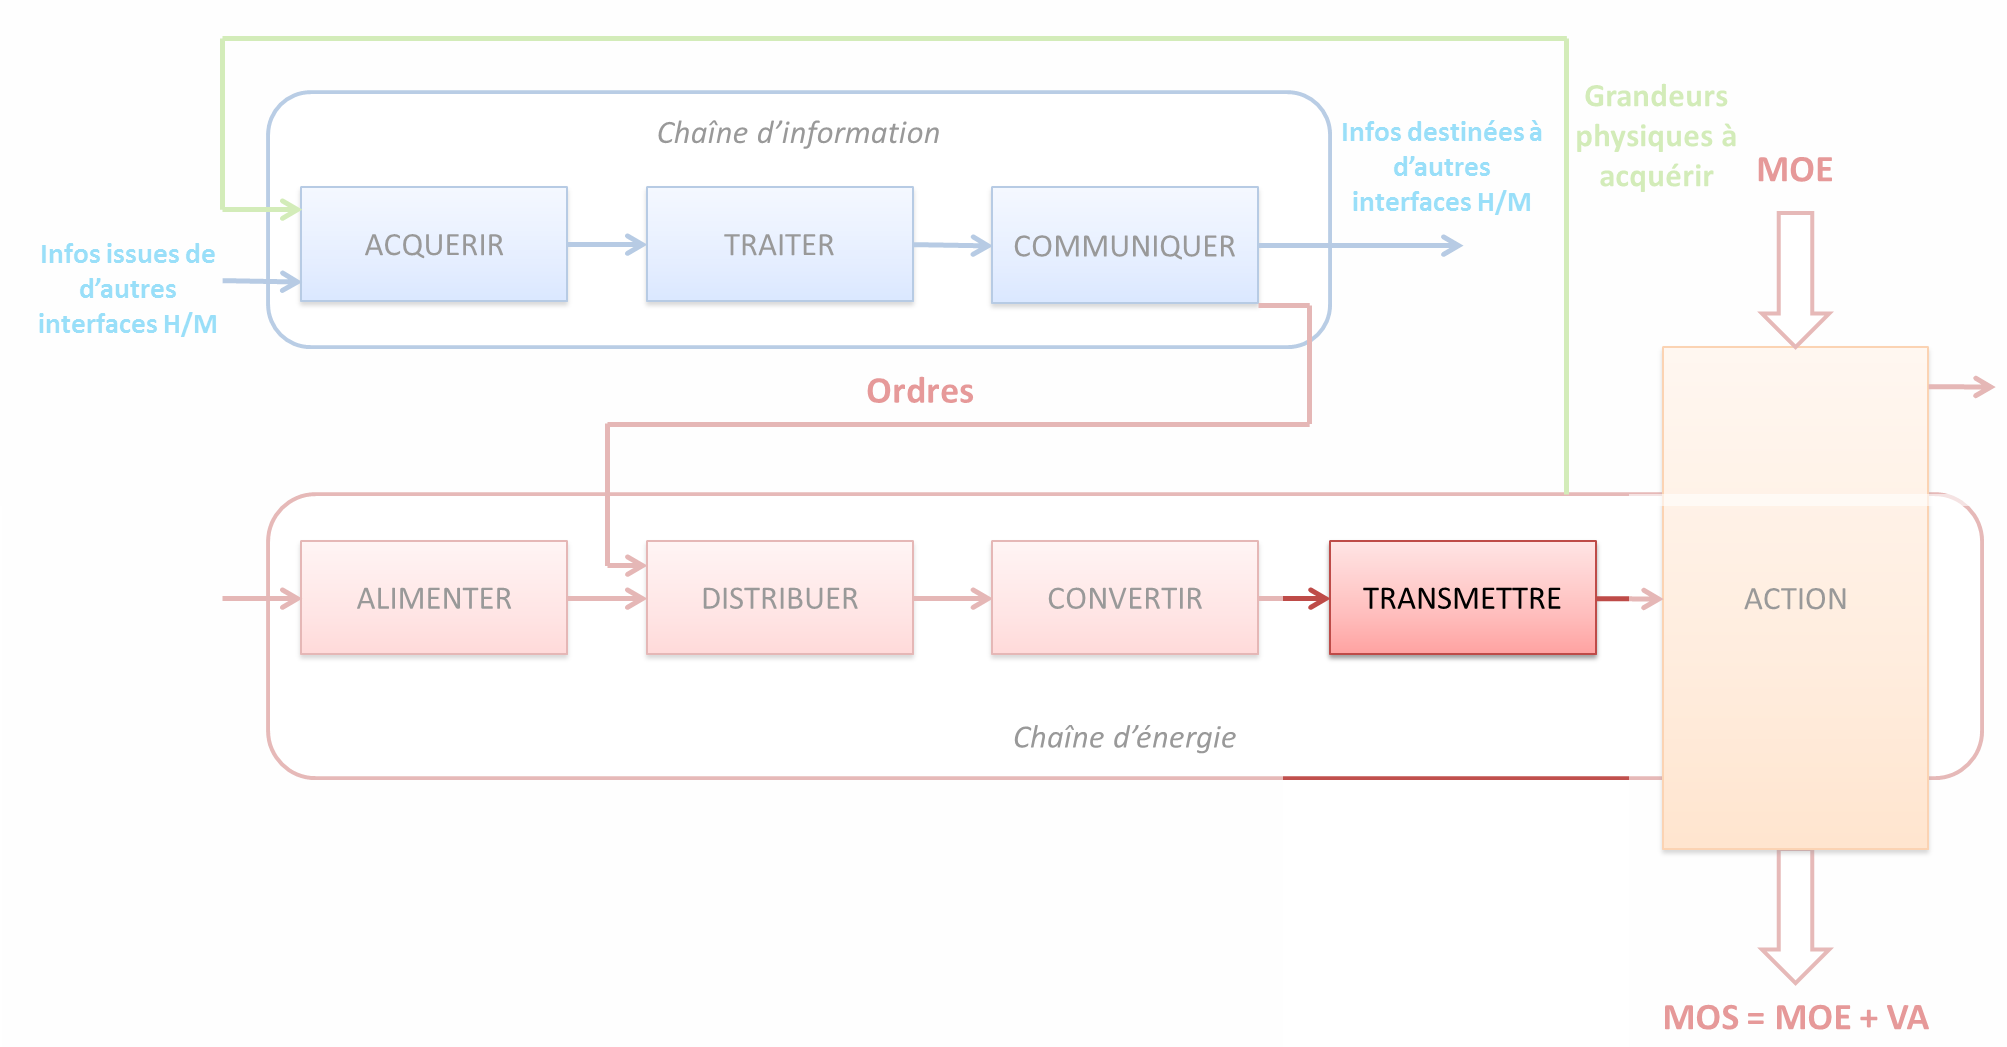
\includegraphics[width=15cm]{png/transmettre}
\end{center}
\vspace{.5cm}

\begin{minipage}[c]{.22\linewidth}
\begin{center}
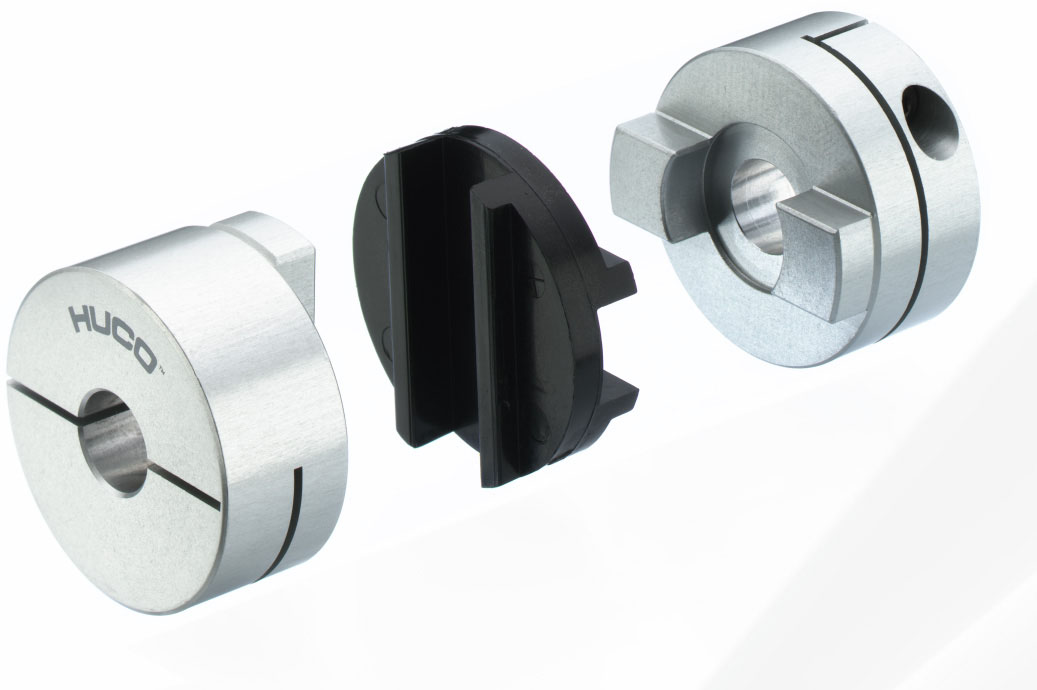
\includegraphics[height=3cm]{png/img_01}

\textit{Joint de Oldham\cite{oldham}}
\end{center}
\end{minipage} \hfill
\begin{minipage}[c]{.22\linewidth}
\begin{center}
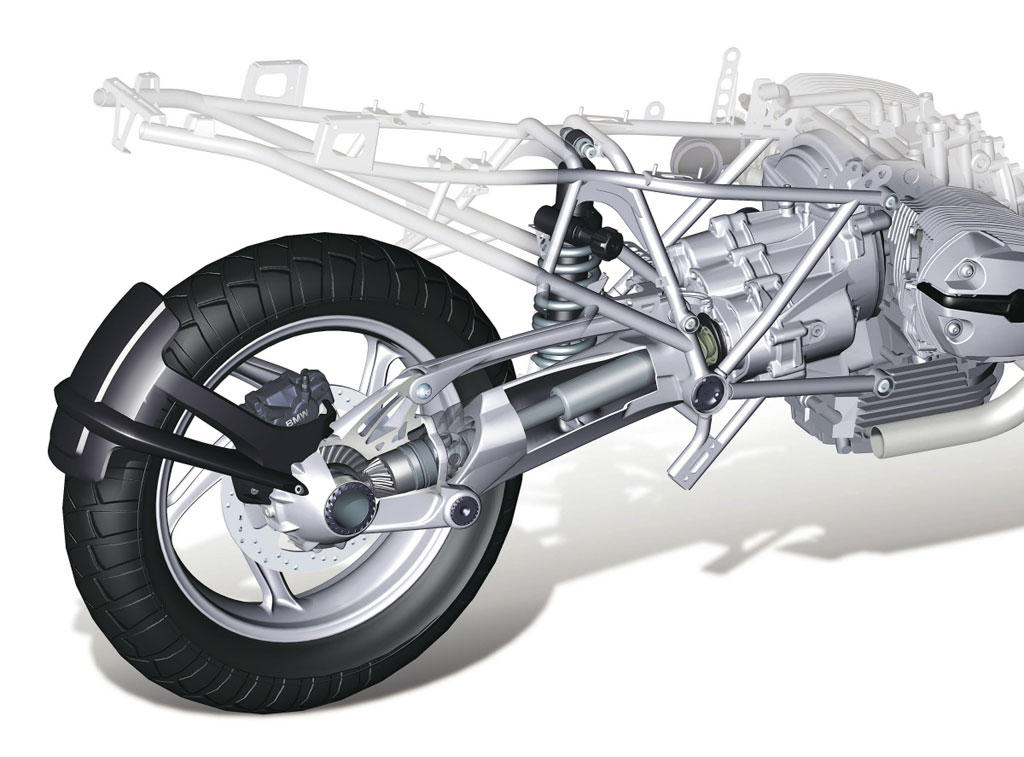
\includegraphics[height=3cm]{png/img_02}

\textit{Transmission de BMW\cite{bmw}}
\end{center}
\end{minipage} \hfill
\begin{minipage}[c]{.22\linewidth}
\begin{center}
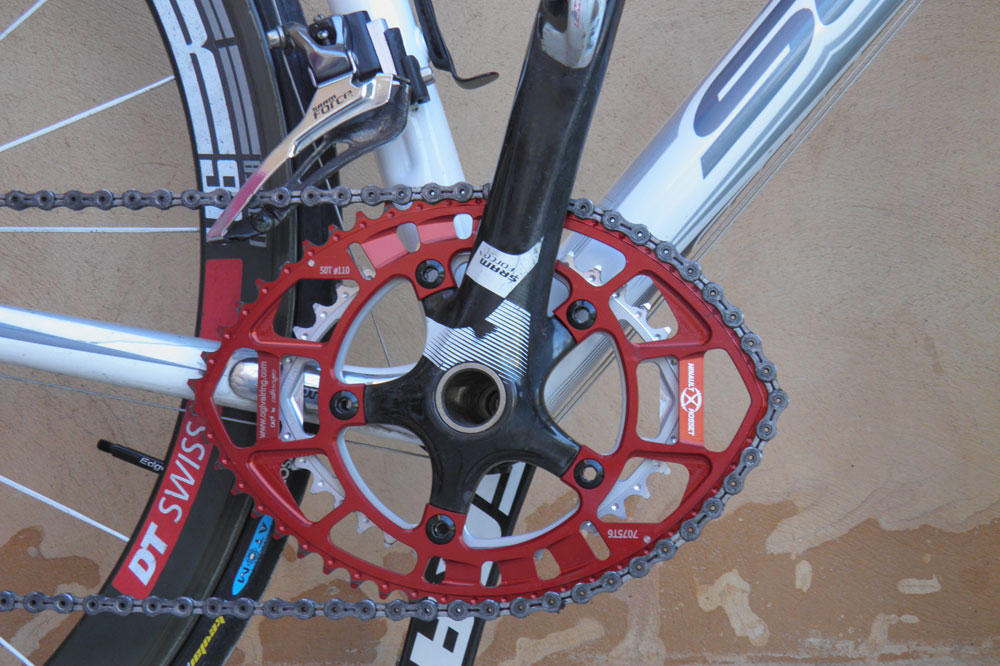
\includegraphics[height=3cm]{png/img_03}

\textit{Plateau ovale "Ogival"\cite{ogival}}
\end{center}
\end{minipage} \hfill
\begin{minipage}[c]{.22\linewidth}
\begin{center}
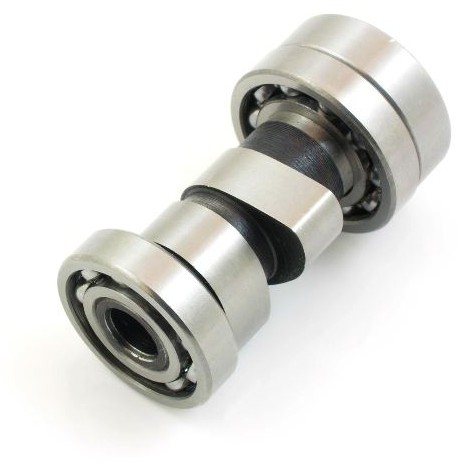
\includegraphics[height=3cm]{png/img_04}

\textit{Arbre à cames de Honda Gorilla\cite{came}}
\end{center}
\end{minipage} 

\vspace{.25cm}


%\begin{center}
%\includegraphics[width=.9\textwidth]{png/cyclev.png}

%\textit{Cycle de conception d'un produit}
%\end{center}

%\begin{prob}
%\textsc{Problématique :}
%\begin{itemize}
%\item %Quelles sont les conditions fonctionnelles permettant le fonctionnement du système ?
%\item %Quelle est la chaîne de côte unidirectionnelle correspondant à une condition donnée ?
%\end{itemize}
%\end{prob}



\begin{savoir}
\textsc{Savoirs :}
\begin{itemize}
\item Principes physiques et caractéristiques de la transmission d'énergie.
\end{itemize}
\end{savoir}
 

\setlength{\parskip}{0ex plus 0.2ex minus 0ex}
 \renewcommand{\contentsname}{}
 \renewcommand{\baselinestretch}{1}

\tableofcontents

 \renewcommand{\baselinestretch}{1.2}
\setlength{\parskip}{2ex plus 0.5ex minus 0.2ex}

% \vspace{1cm}
\textit{Ce document évolue. Merci de signaler toutes erreurs ou coquilles.}

\section{La transmission de l'énergie sans transformation de mouvement et sans modification de la vitesse de rotation}


\subsection{Arbres et axes}

Les arbres sont des pièces mécaniques, de section généralement circulaire.
On distingue principalement deux familles d’arbres :
\begin{itemize}
\item ceux qui transmettent un couple entre les éléments de transmission qu’ils supportent : poulies, pignons, joints d’accouplement, … ;
\item ceux qui ne transmettent pas de couple, on les appelle alors des axes, ils servent de support d’organes mécaniques ou bien d’axes d’articulation.
\end{itemize}

\begin{minipage}[c]{.6\linewidth}
\begin{center}
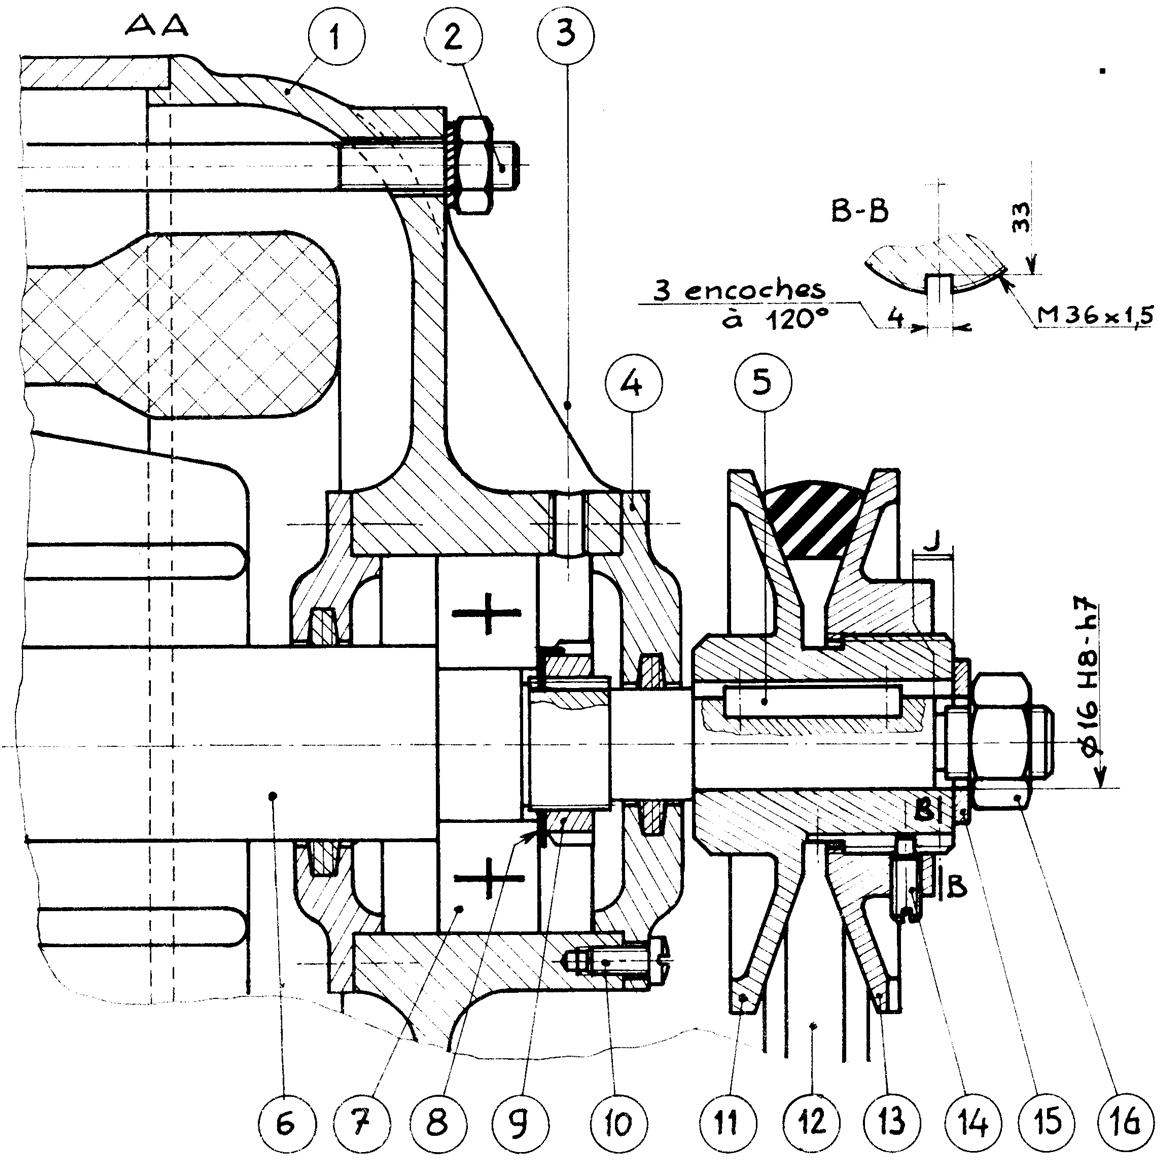
\includegraphics[width=.9\textwidth]{png/fig_01}
%\textit{Cycle de conception d'un produit}
\end{center}
 \end{minipage} \hfill
\begin{minipage}[c]{.35\linewidth}
\begin{center}
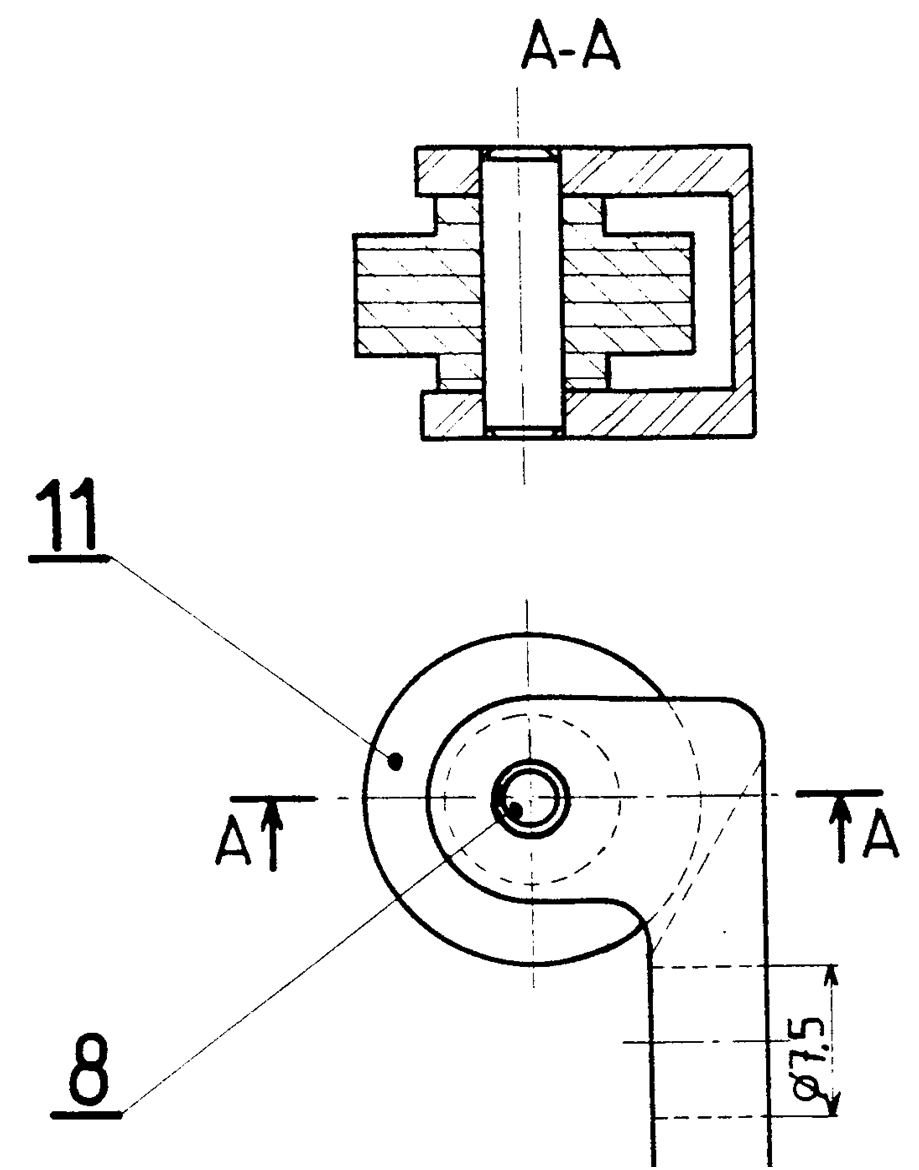
\includegraphics[width=.8\textwidth]{png/fig_02}
%\textit{Cycle de conception d'un produit}
\end{center}
 \end{minipage}

Le dimensionnement des arbres s’effectue soit par un calcul de résistance des matériaux, soit par résolution numérique sur logiciel de calcul par éléments finis.

\paragraph*{Matériaux utilisés pour la fabrication des arbres}
Les arbres sont en général en acier d’usage courant pour des applications non soumises à des exigences particulières, trempés ou cémentés pour d’autres plus exigeantes. 

Pour certaines applications (aéronautique, automobile de compétition, …), on peut avoir recours à l’utilisation de matériaux composites (PRFC) ou d’alliages de titane.

Le choix d’un matériau adéquat dépend des dimensions, l’usinabilité, la soudabilité, l’aptitude aux traitements thermiques, les conditions de fonctionnement (chocs, fatigue, etc.).

\subsection{Les accouplements entre arbres alignés}

Ces accouplements assurent la transmission de puissance entre deux arbres de transmission alignés ou possédant quelques défauts d’alignement.

La puissance à transmettre est donnée par la formule $\mathcal{P}=C\omega$  (solide tournant autour d’un axe fixe, $\mathcal{P}$ en Watt, $C$, en $N.m$, $\omega$ en $rad/s$).

Les défauts d’alignement peuvent être de type : radial, axial, angulaire, écart angulaire en torsion :

\noindent\begin{minipage}[c]{.3\linewidth}
\begin{center}
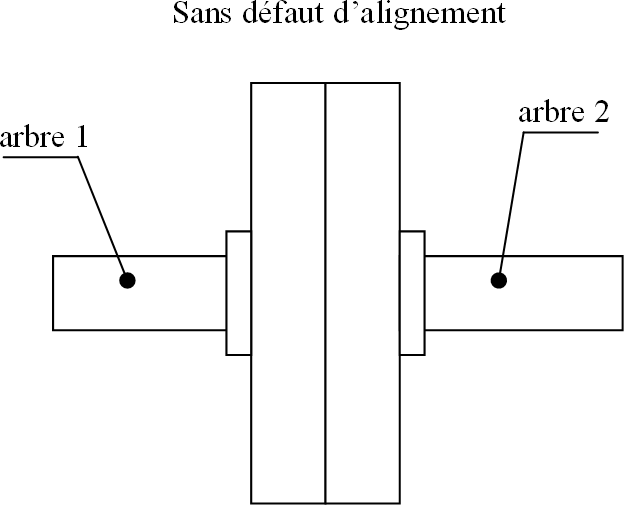
\includegraphics[height=4cm]{png/fig_03}
%\textit{}
\end{center}
\end{minipage} \hfill
\begin{minipage}[c]{.3\linewidth}
\begin{center}
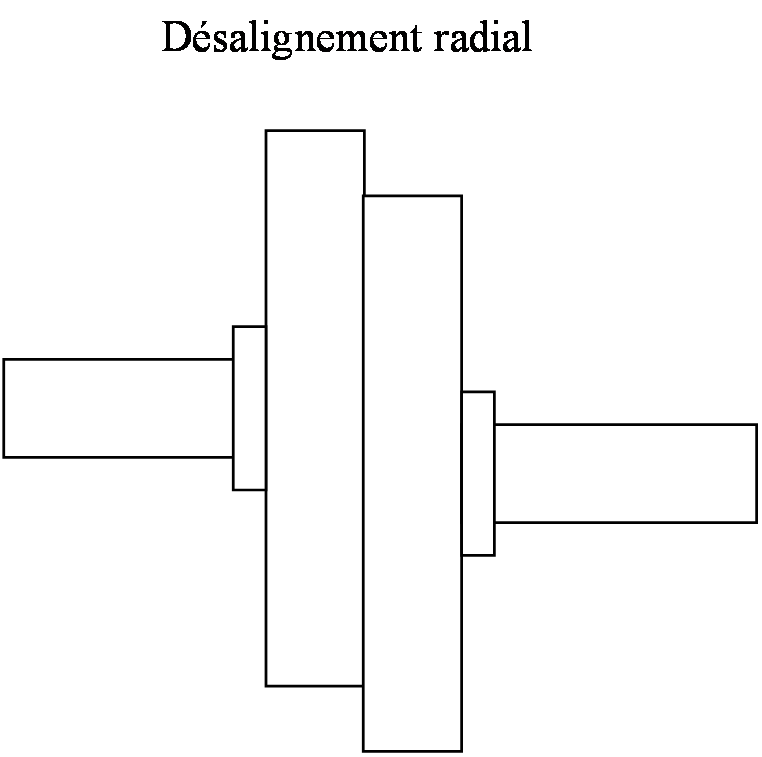
\includegraphics[height=4cm]{png/fig_05}
%\textit{}
\end{center}
\end{minipage} \hfill
\begin{minipage}[c]{.3\linewidth}
\begin{center}
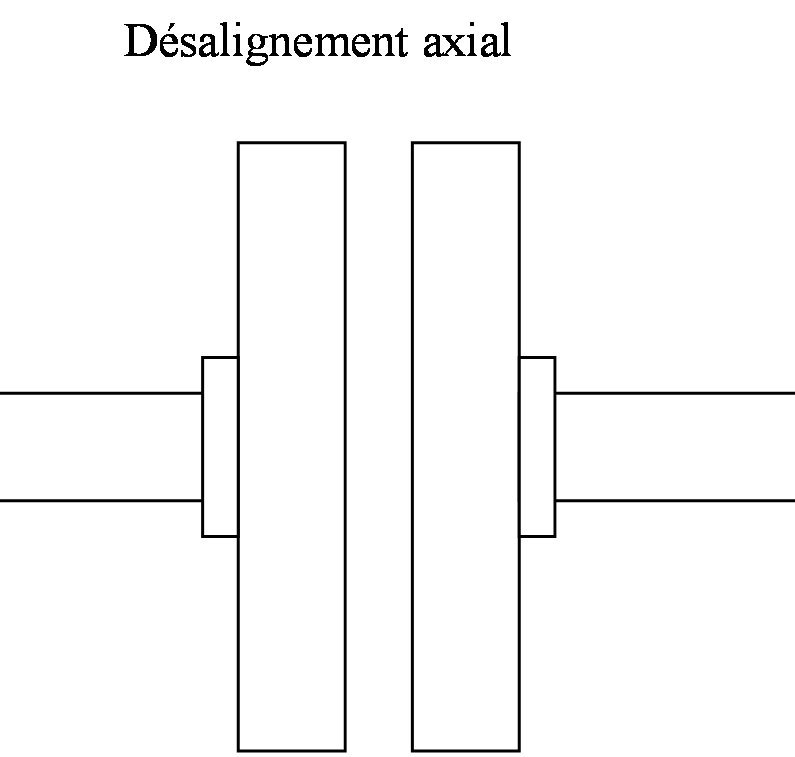
\includegraphics[height=4cm]{png/fig_06}
%\textit{}
\end{center}
\end{minipage} 


\begin{minipage}[c]{.45\linewidth}
\begin{center}
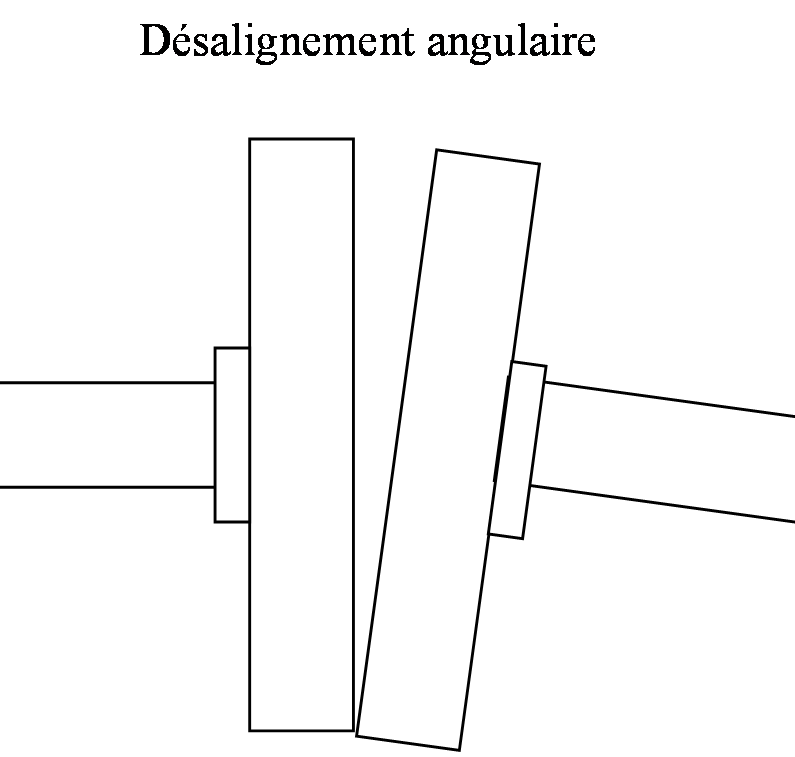
\includegraphics[height=4cm]{png/fig_07}
%\textit{}
\end{center}
\end{minipage} \hfill
\begin{minipage}[c]{.45\linewidth}
\begin{center}
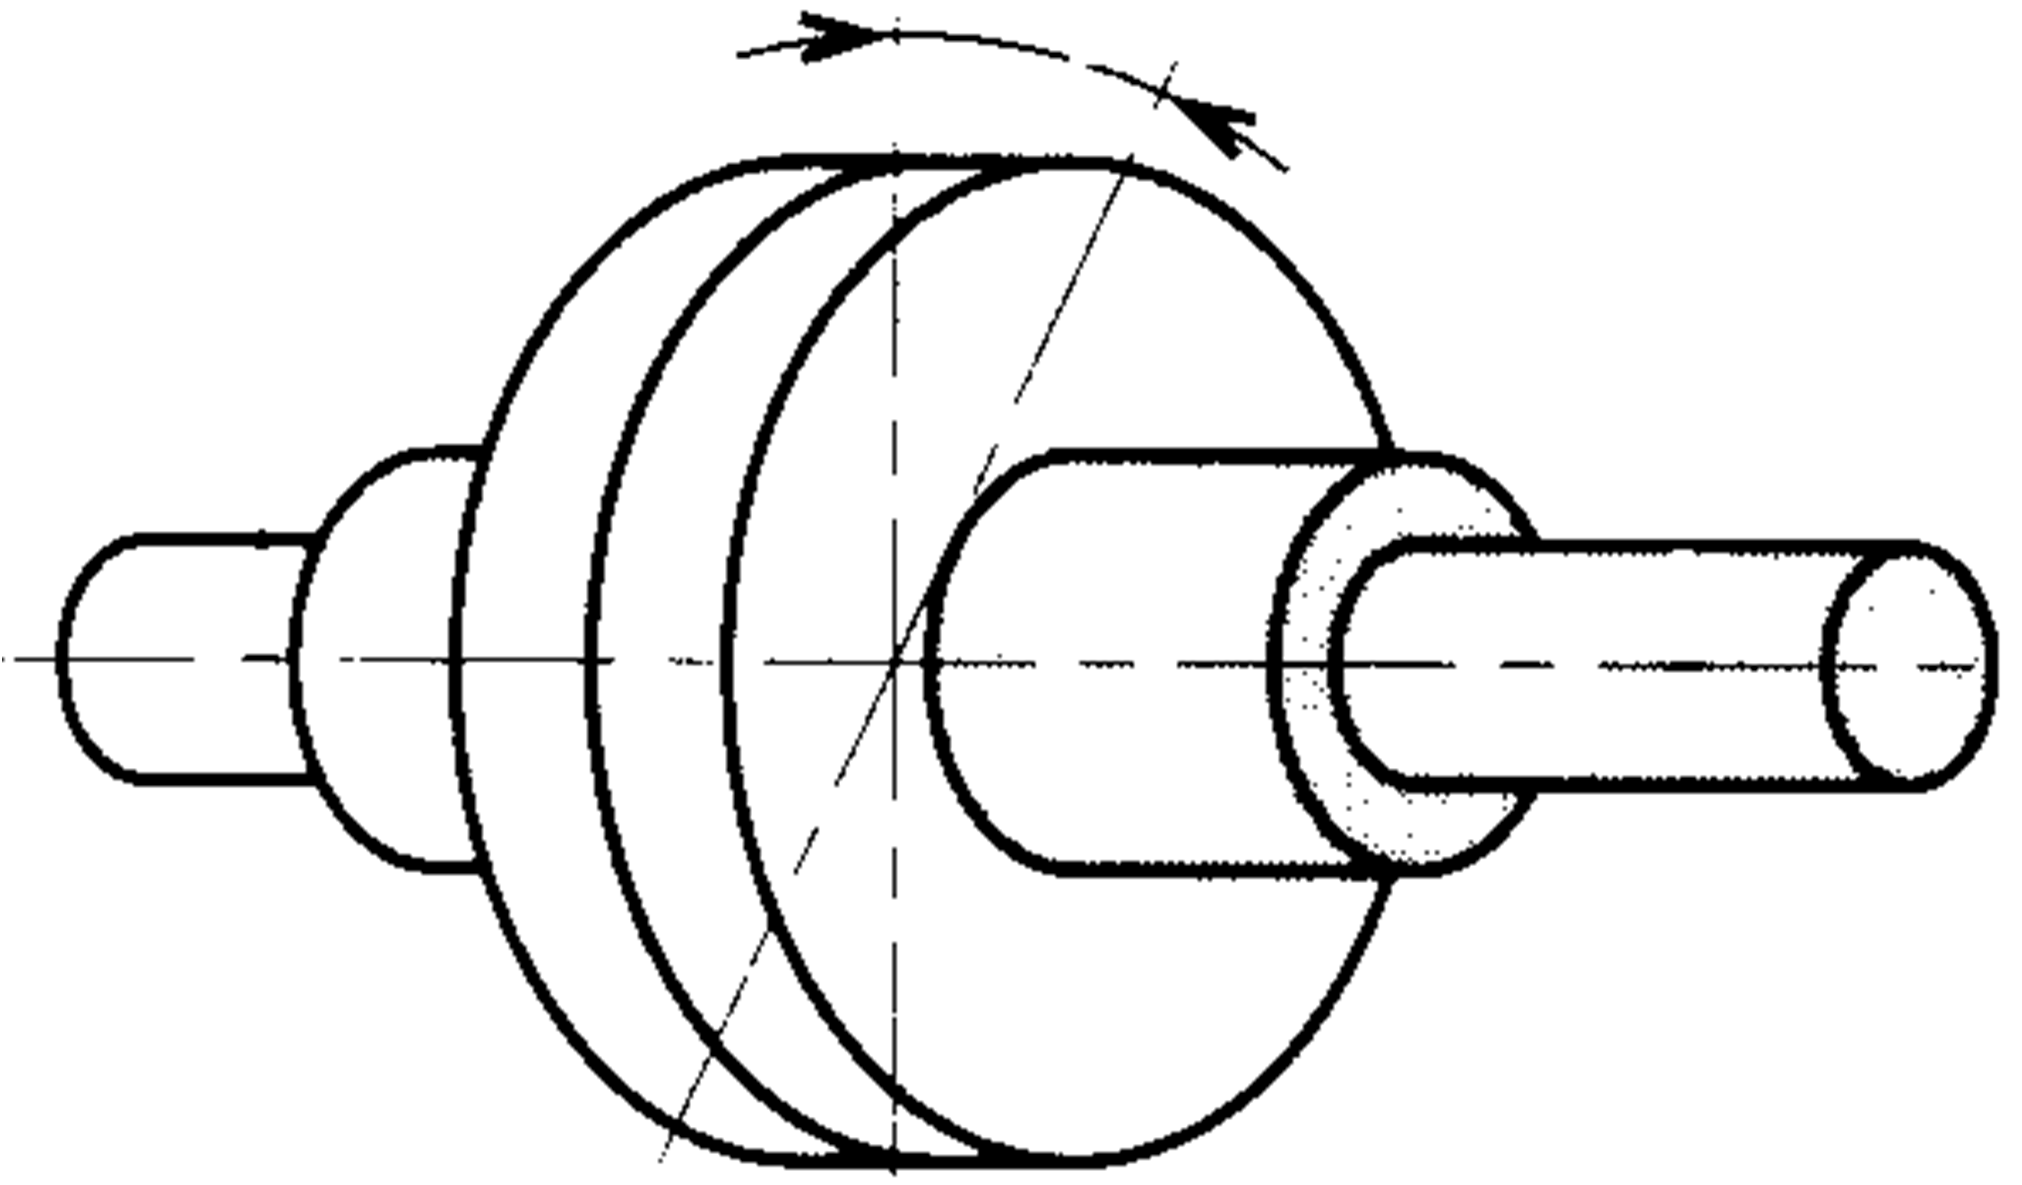
\includegraphics[height=4cm]{png/fig_08}
%\textit{}
\end{center}
\end{minipage}

\subsubsection{Les accouplements permanents}
Dans le cas d’un accouplement permanent, le désaccouplement n’est possible qu’après démontage.
\paragraph{Les accouplements rigides}

Ils ne tolèrent pas de défaut d’alignement.

\begin{center}
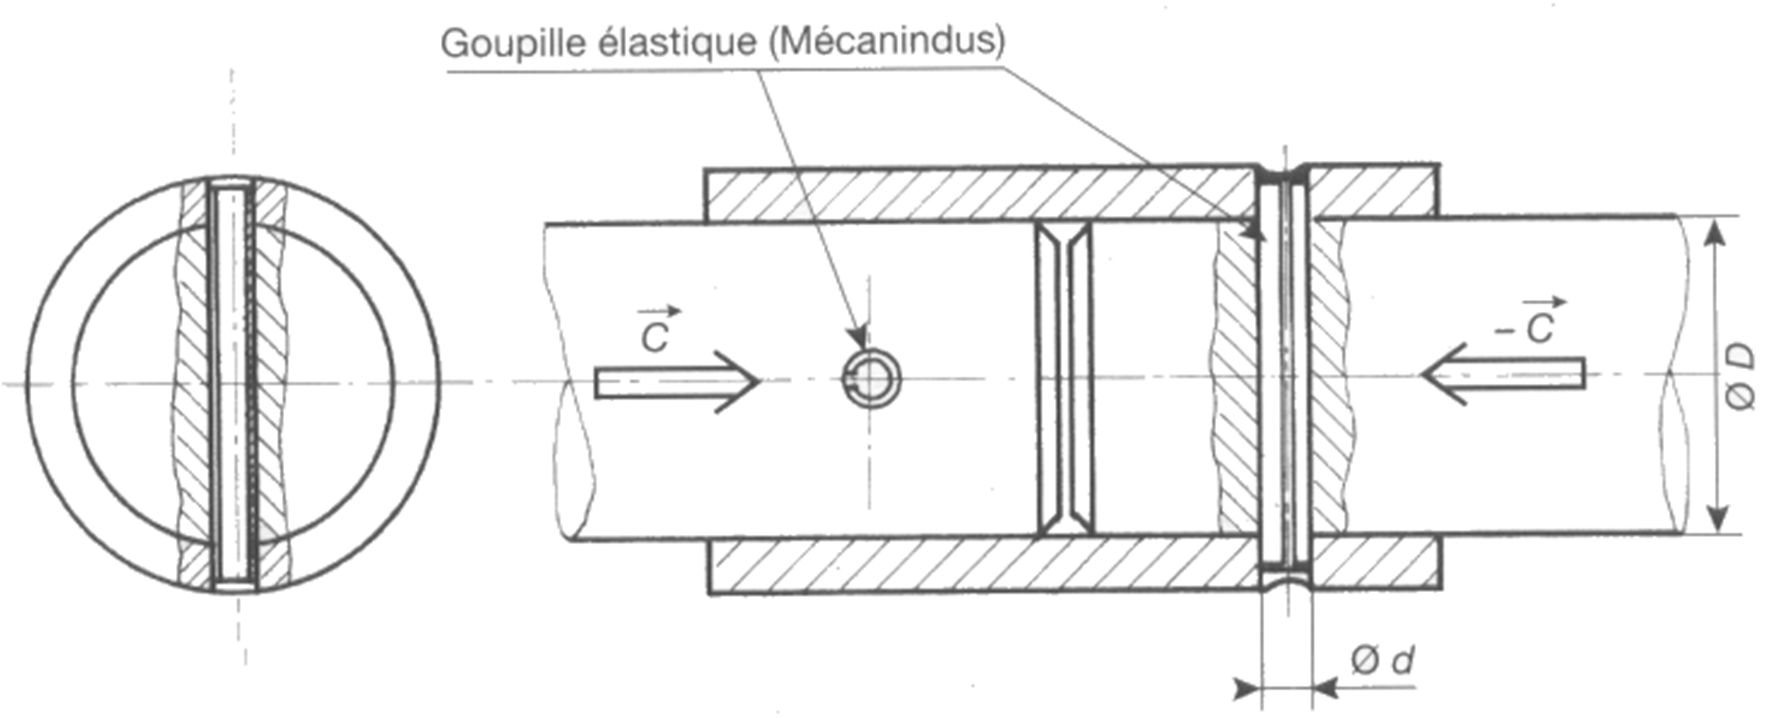
\includegraphics[width=.7\textwidth]{png/fig_09}
%\textit{}
\end{center}

\begin{minipage}[c]{.4\linewidth}
\begin{center}
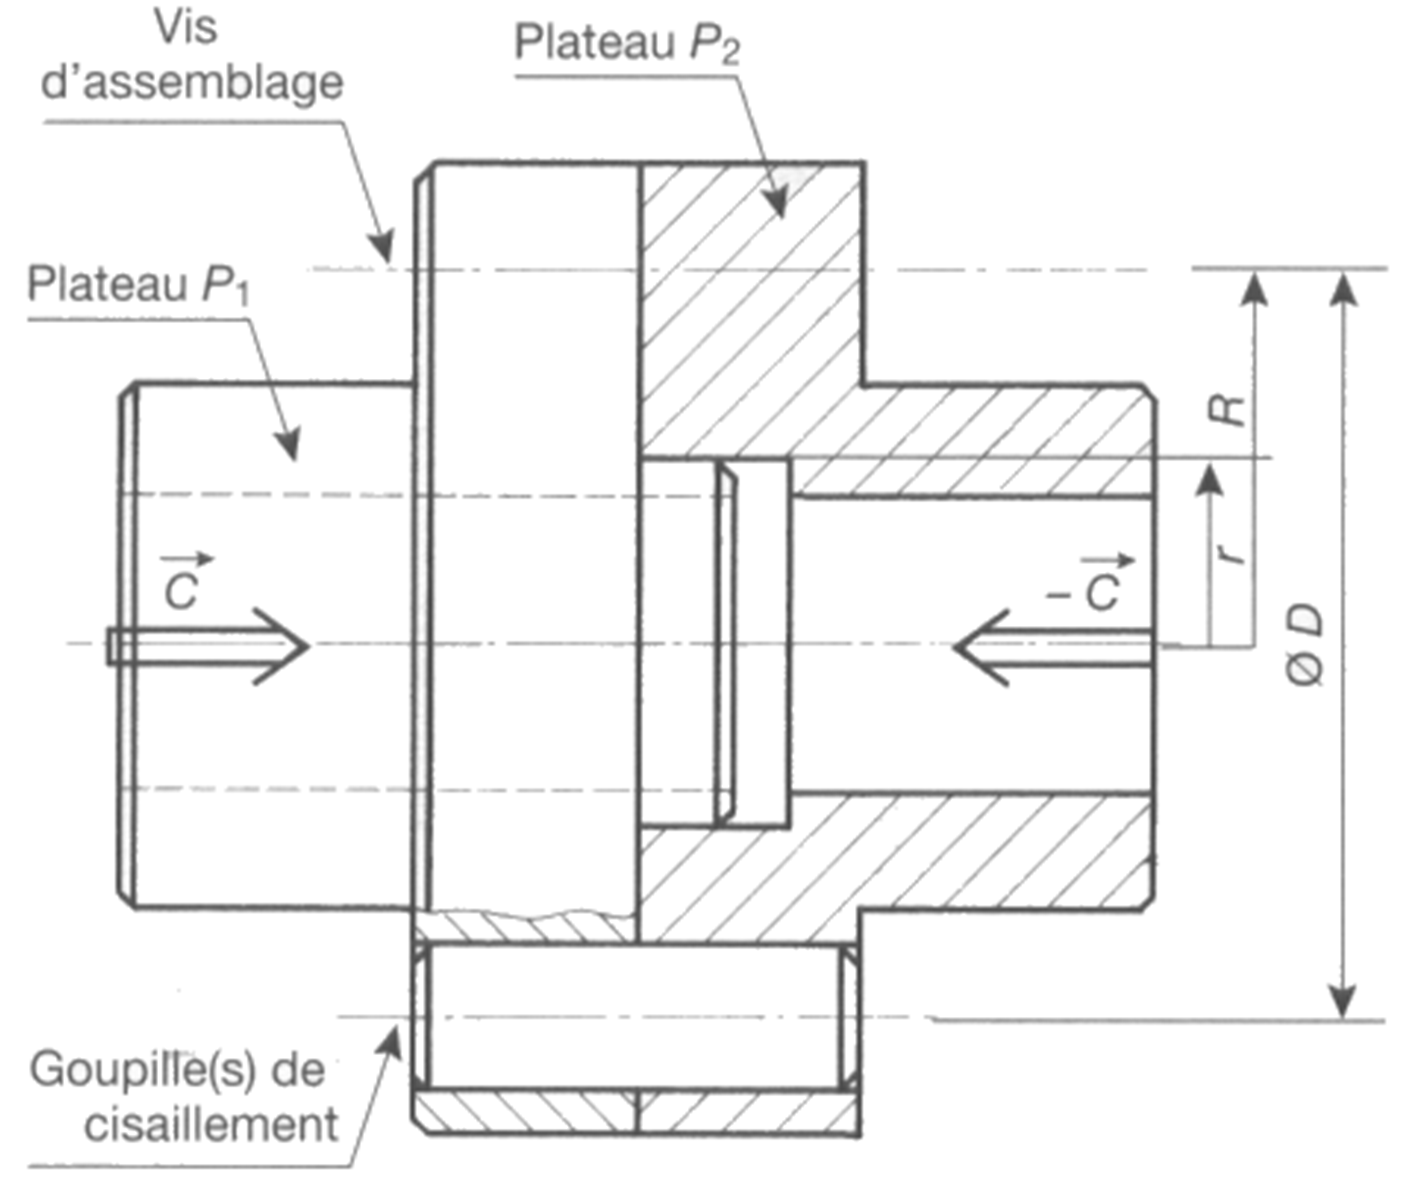
\includegraphics[width=.9\textwidth]{png/fig_10}
%\textit{}
\end{center}
\end{minipage} \hfill
\begin{minipage}[c]{.55\linewidth}
Les goupilles réalisent la transmission du couple.
Les vis d’assemblage réalisent uniquement le maintien en position des deux plateaux et ne participent pas à la transmission du couple.
\end{minipage}

\paragraph{Les accouplements élastiques, flexibles et joints d’accouplement positifs}
Ils tolèrent certains défauts d’alignement.


\noindent\begin{minipage}[c]{.25\linewidth}
\begin{center}
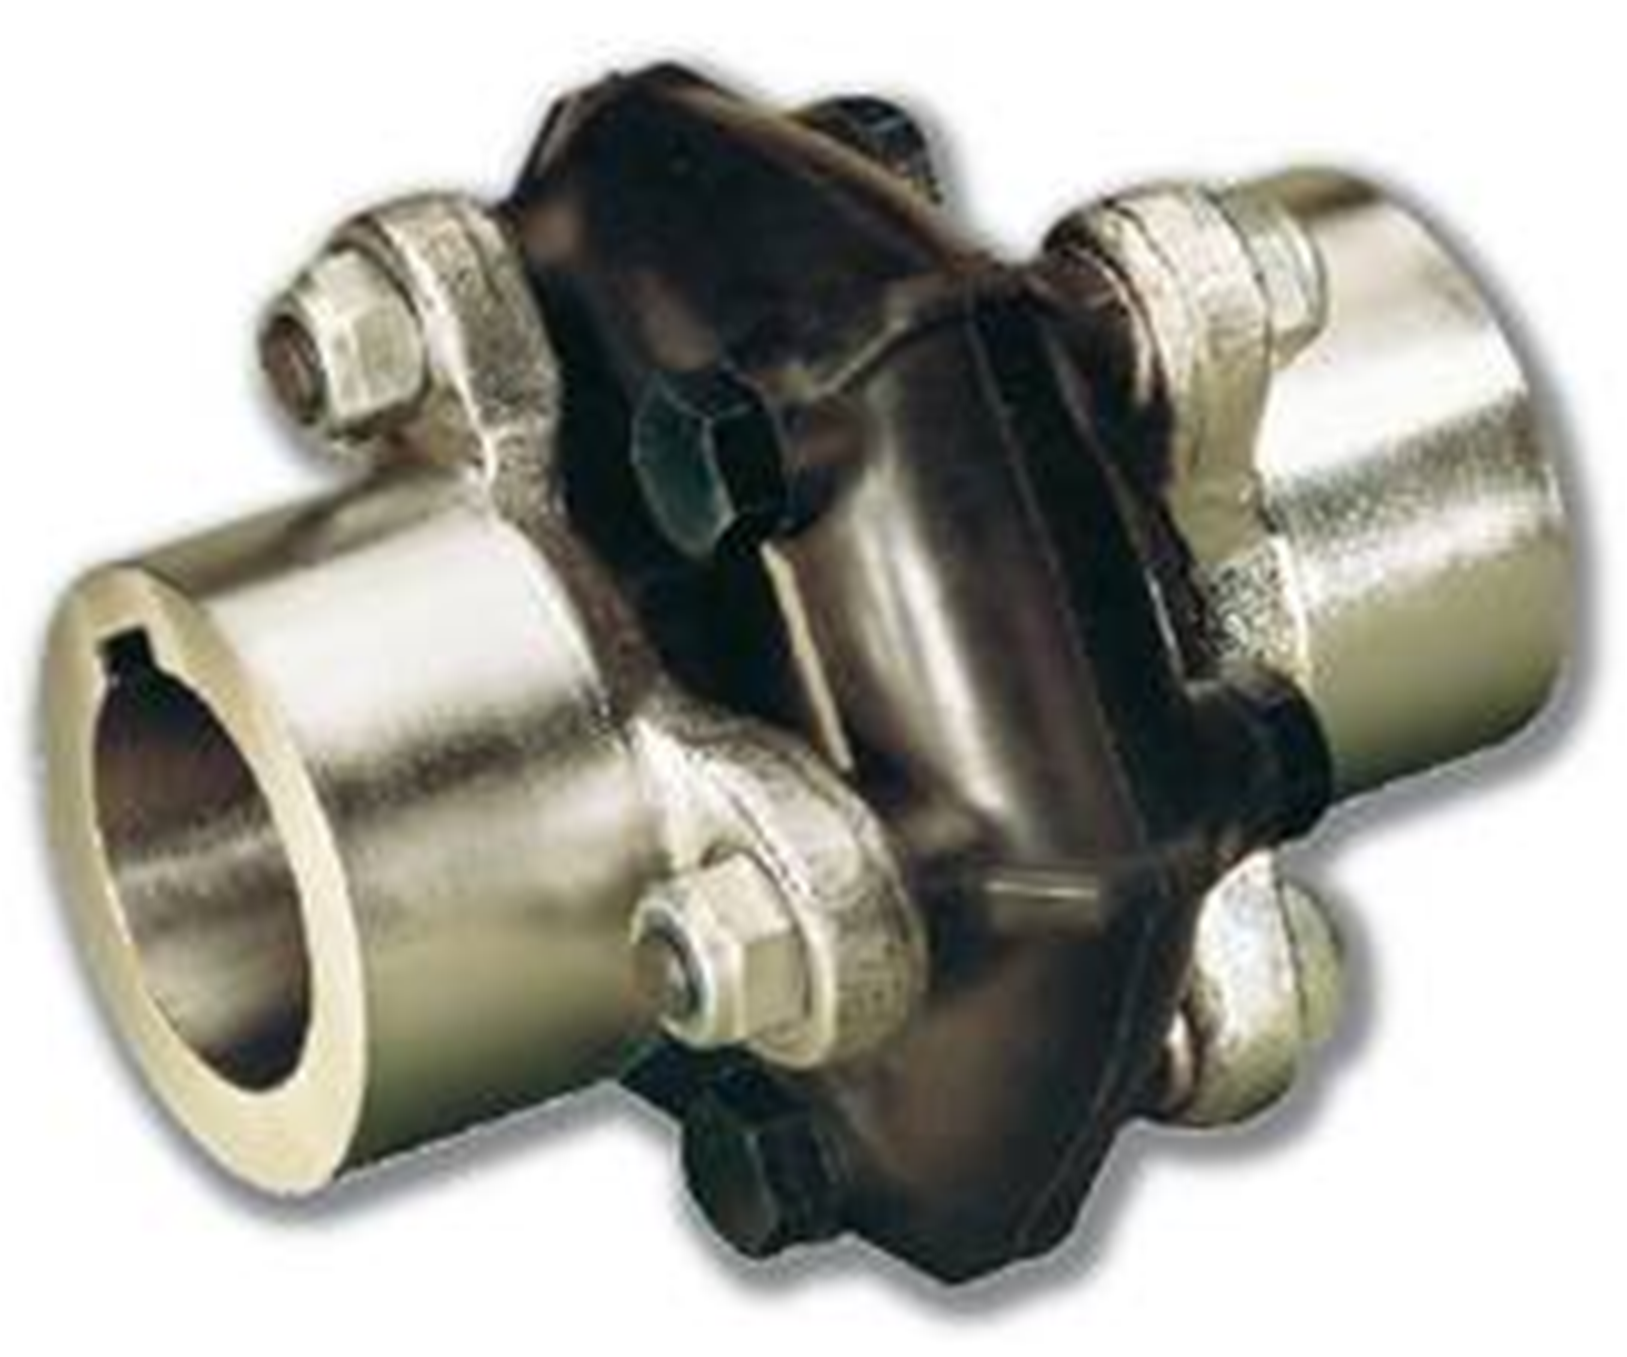
\includegraphics[height=4cm]{png/fig_11}
%\textit{}
\end{center}
\end{minipage} \hfill
\begin{minipage}[c]{.4\linewidth}
\begin{center}
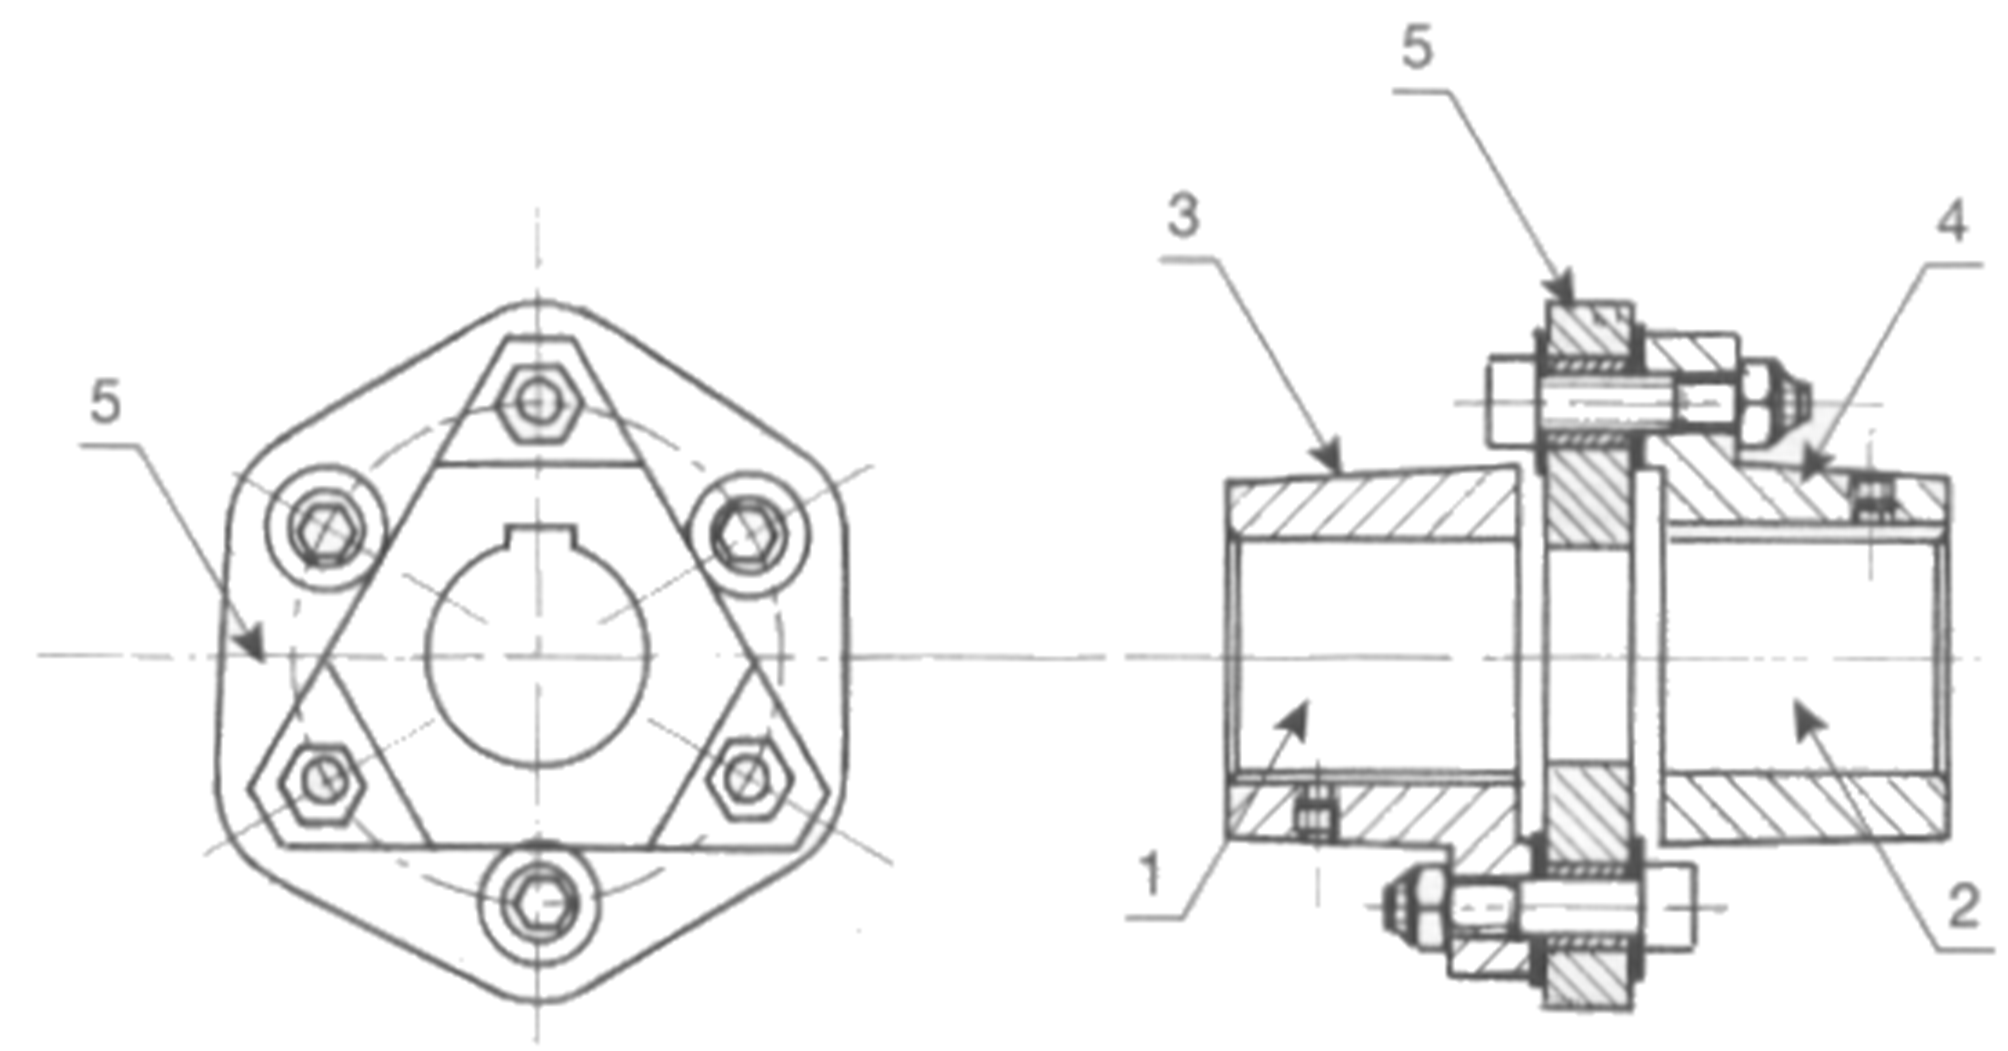
\includegraphics[height=4cm]{png/fig_12}
%\textit{}
\end{center}
\end{minipage}\hfill
\begin{minipage}[c]{.3\linewidth}
Désalignement radial : 
$\Delta r = \pm 0,3\; mm$

Désalignement axial : 
$\Delta a = \pm 4\; mm$

Désalignement angulaire : 
$\Delta \alpha = \pm 5^\text{o}$
\end{minipage}



\noindent\begin{minipage}[c]{.25\linewidth}
\begin{center}
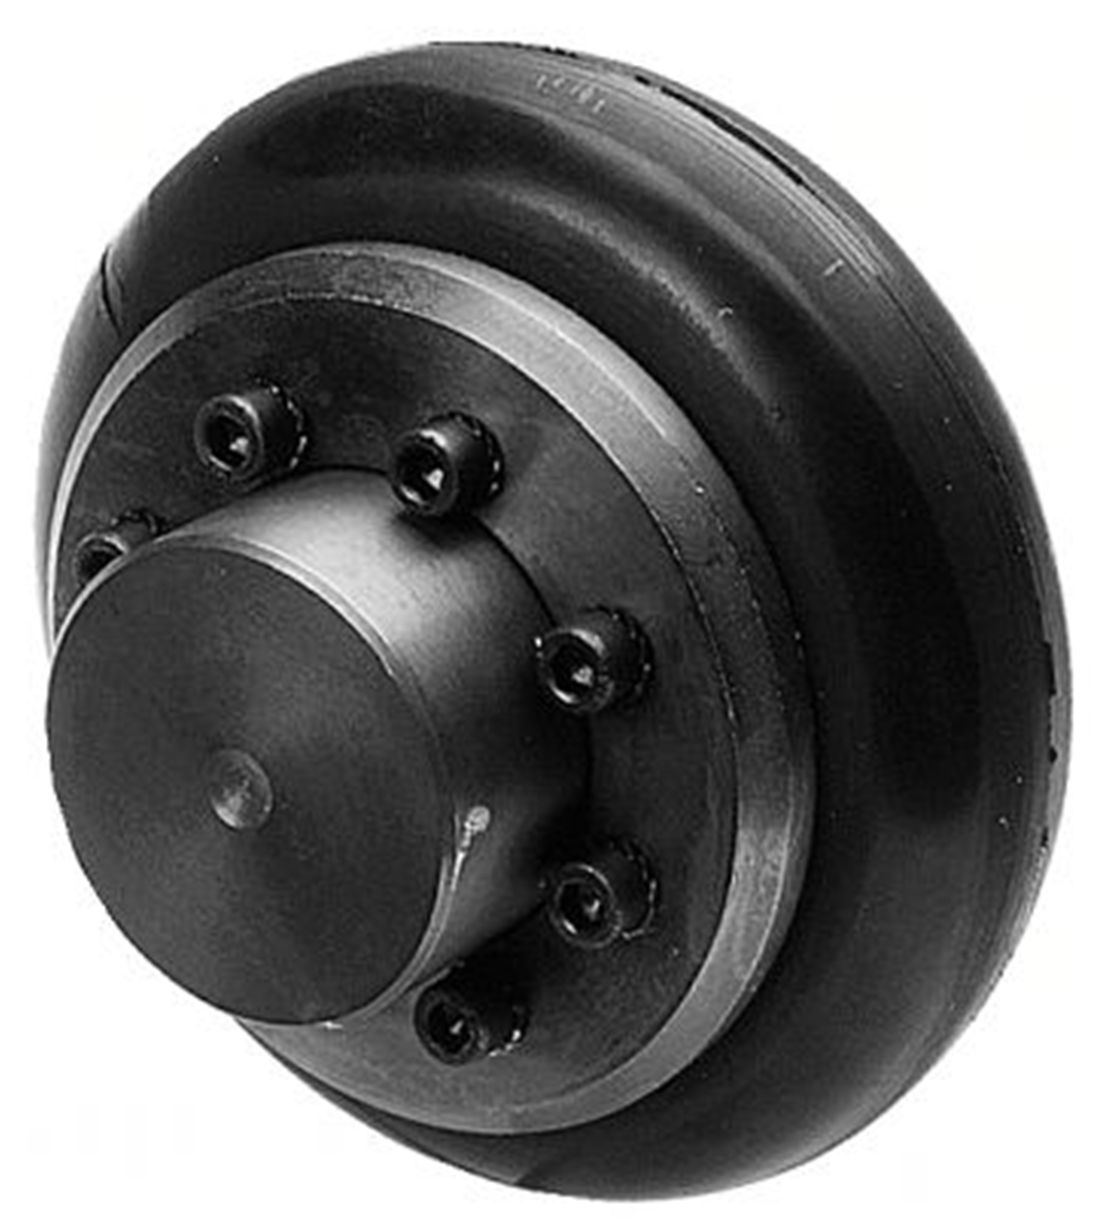
\includegraphics[height=4cm]{png/fig_13}
%\textit{}
\end{center}
\end{minipage} \hfill
\begin{minipage}[c]{.4\linewidth}
\begin{center}
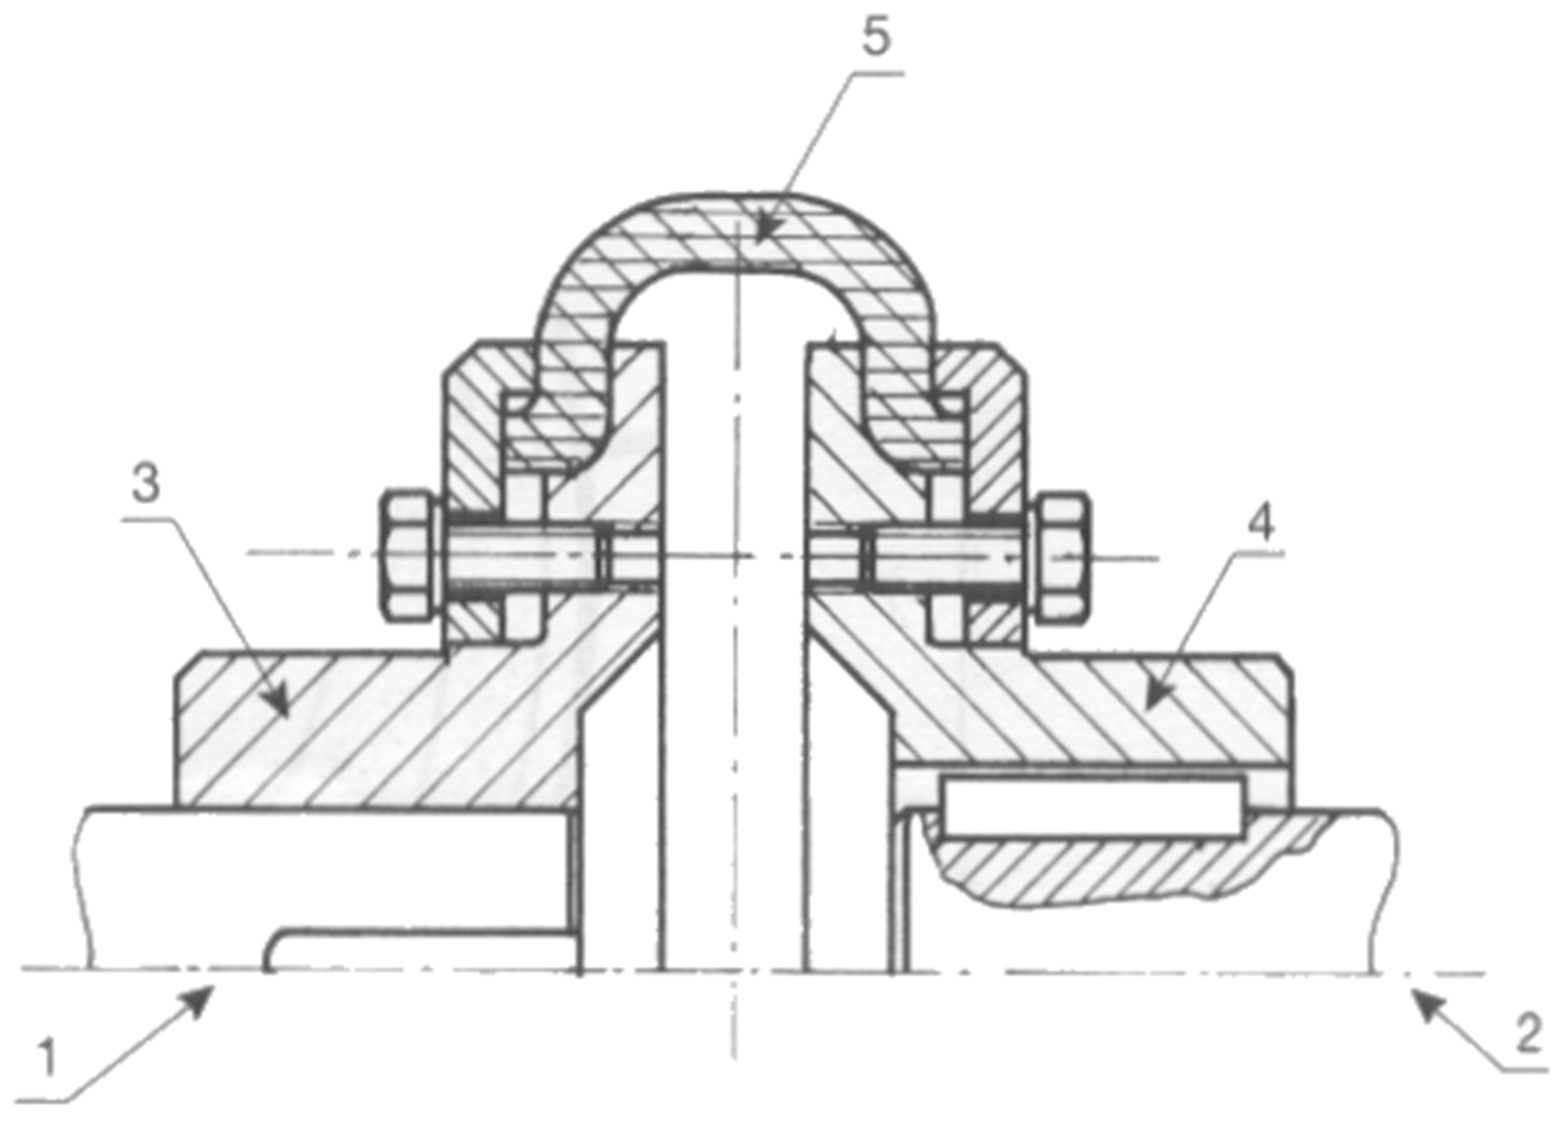
\includegraphics[height=4cm]{png/fig_14}
%\textit{}
\end{center}
\end{minipage}\hfill
\begin{minipage}[c]{.3\linewidth}
Désalignement radial : 
$\Delta r = \pm 5\; mm$

Désalignement axial : 
$\Delta a = \pm 6\; mm$

Désalignement angulaire : 
$\Delta \alpha = \pm 2^\text{o}$
\end{minipage}


\noindent\begin{minipage}[c]{.25\linewidth}
\begin{center}
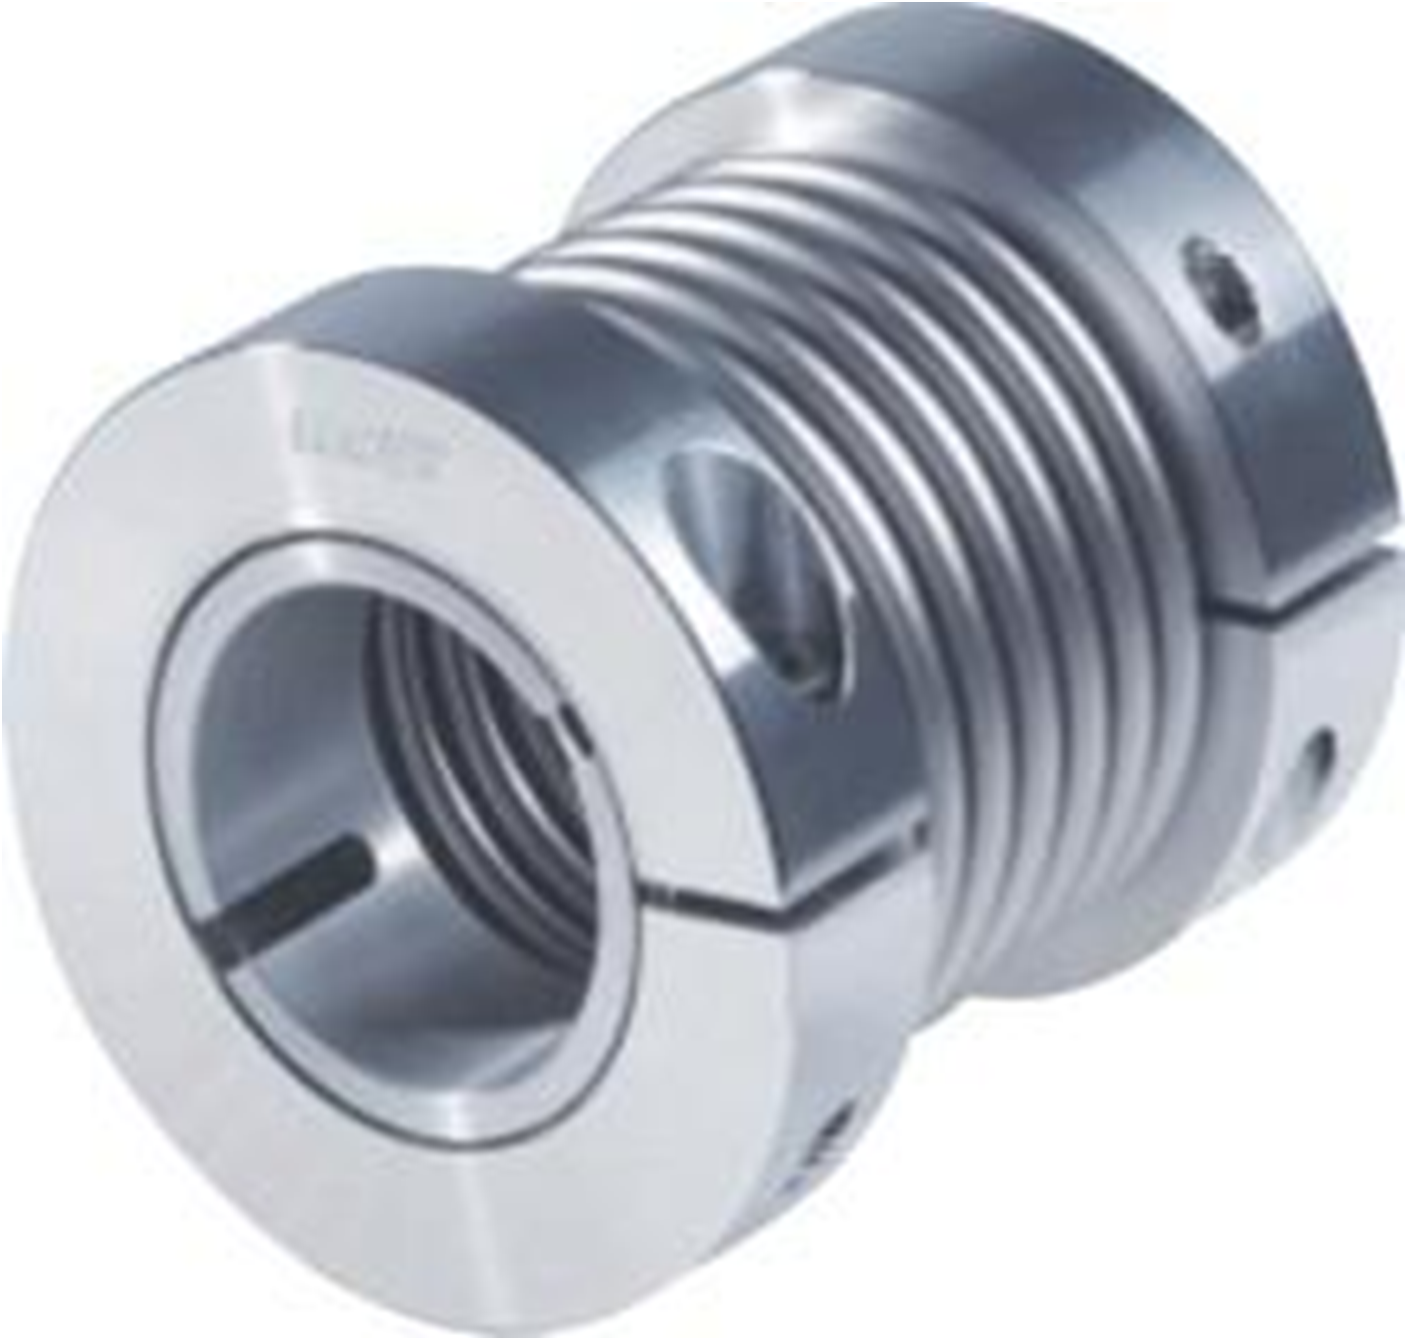
\includegraphics[height=4cm]{png/fig_15}
%\textit{}
\end{center}
\end{minipage} \hfill
\begin{minipage}[c]{.4\linewidth}
\begin{center}
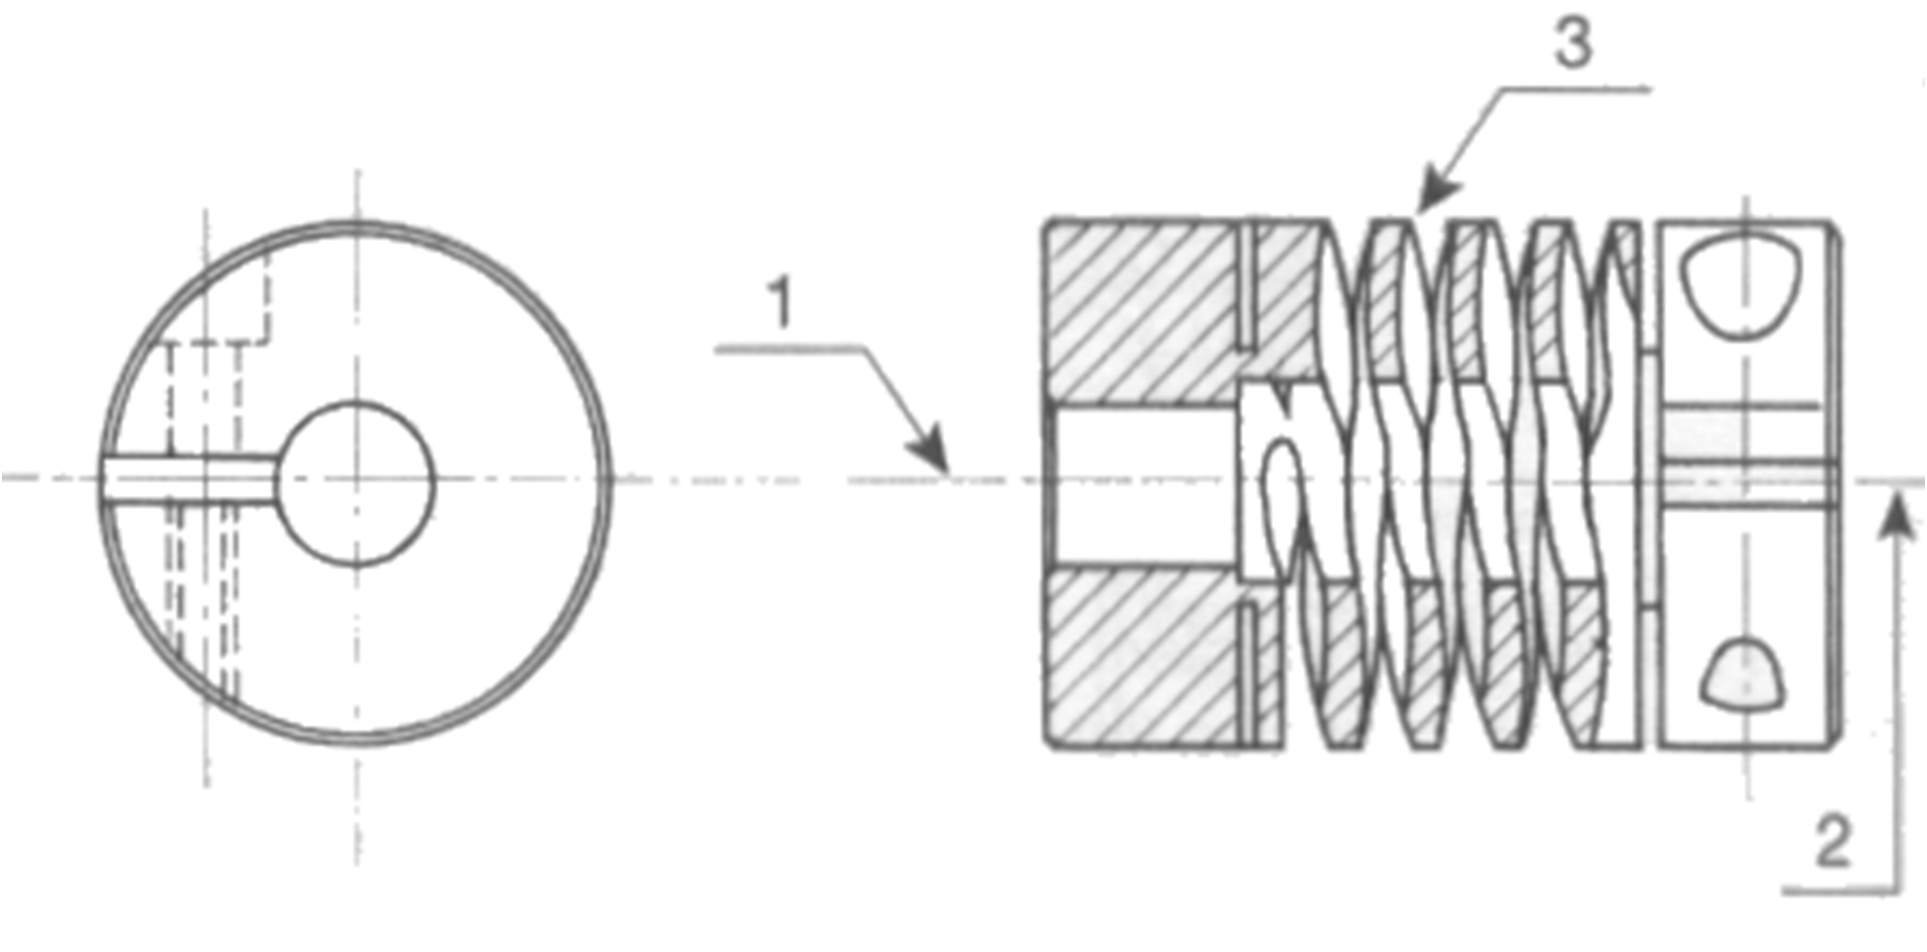
\includegraphics[height=4cm]{png/fig_16}
%\textit{}
\end{center}
\end{minipage}\hfill
\begin{minipage}[c]{.25\linewidth}
Désalignement radial : 
$\Delta r = \pm 3\; mm$

Désalignement axial important

Désalignement angulaire : 
$\Delta \alpha = \pm 30^\text{o}$
\end{minipage}


\noindent \begin{minipage}[c]{.2\linewidth}
\begin{center}
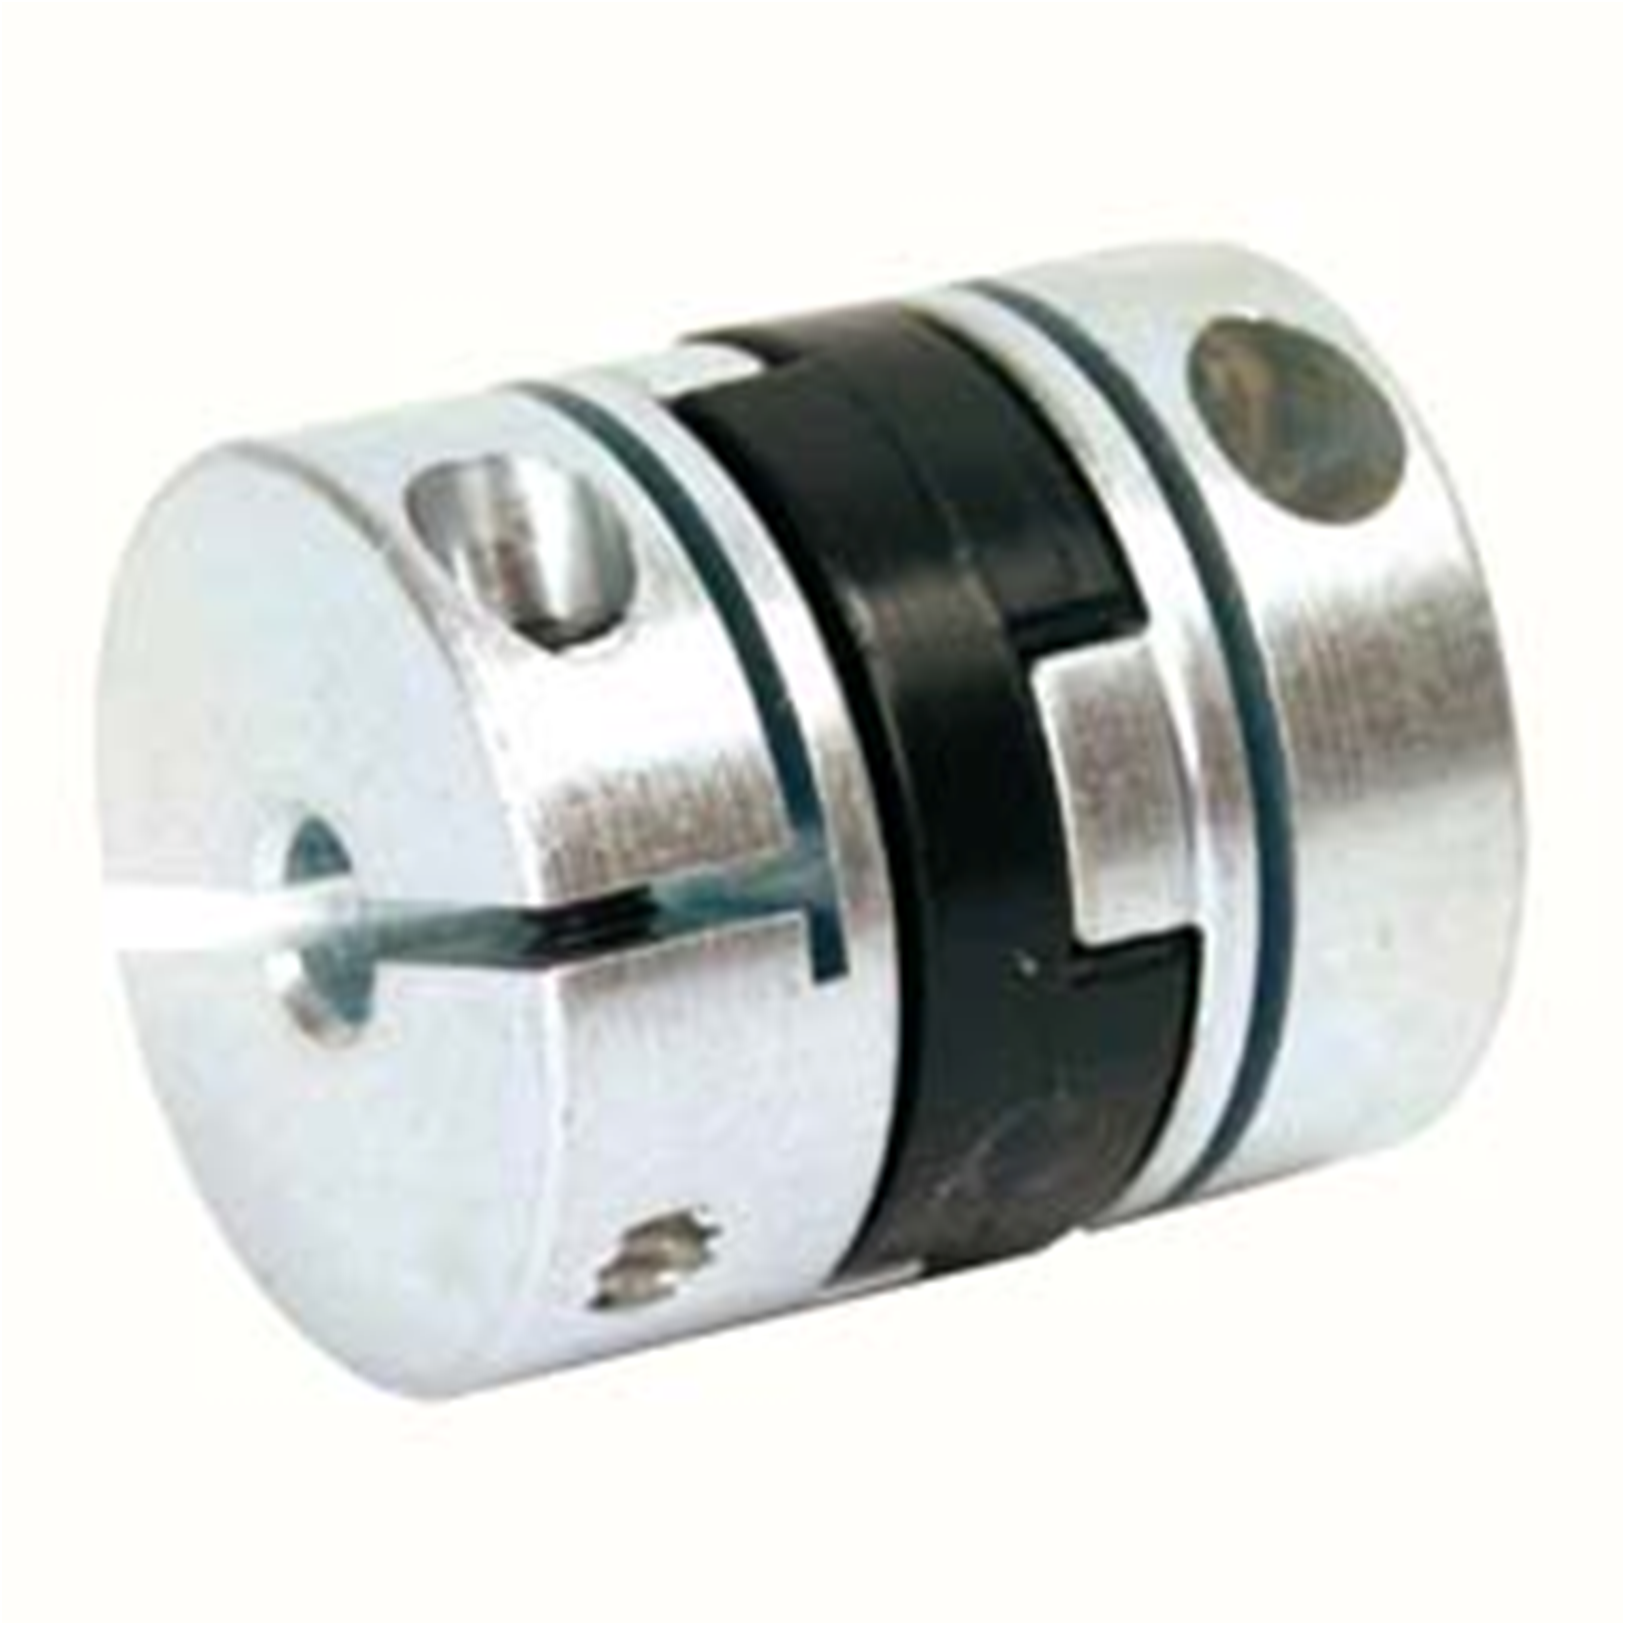
\includegraphics[height=4cm]{png/fig_17}
%\textit{}
\end{center}
\end{minipage} \hfill
\begin{minipage}[c]{.75\linewidth}
\begin{center}
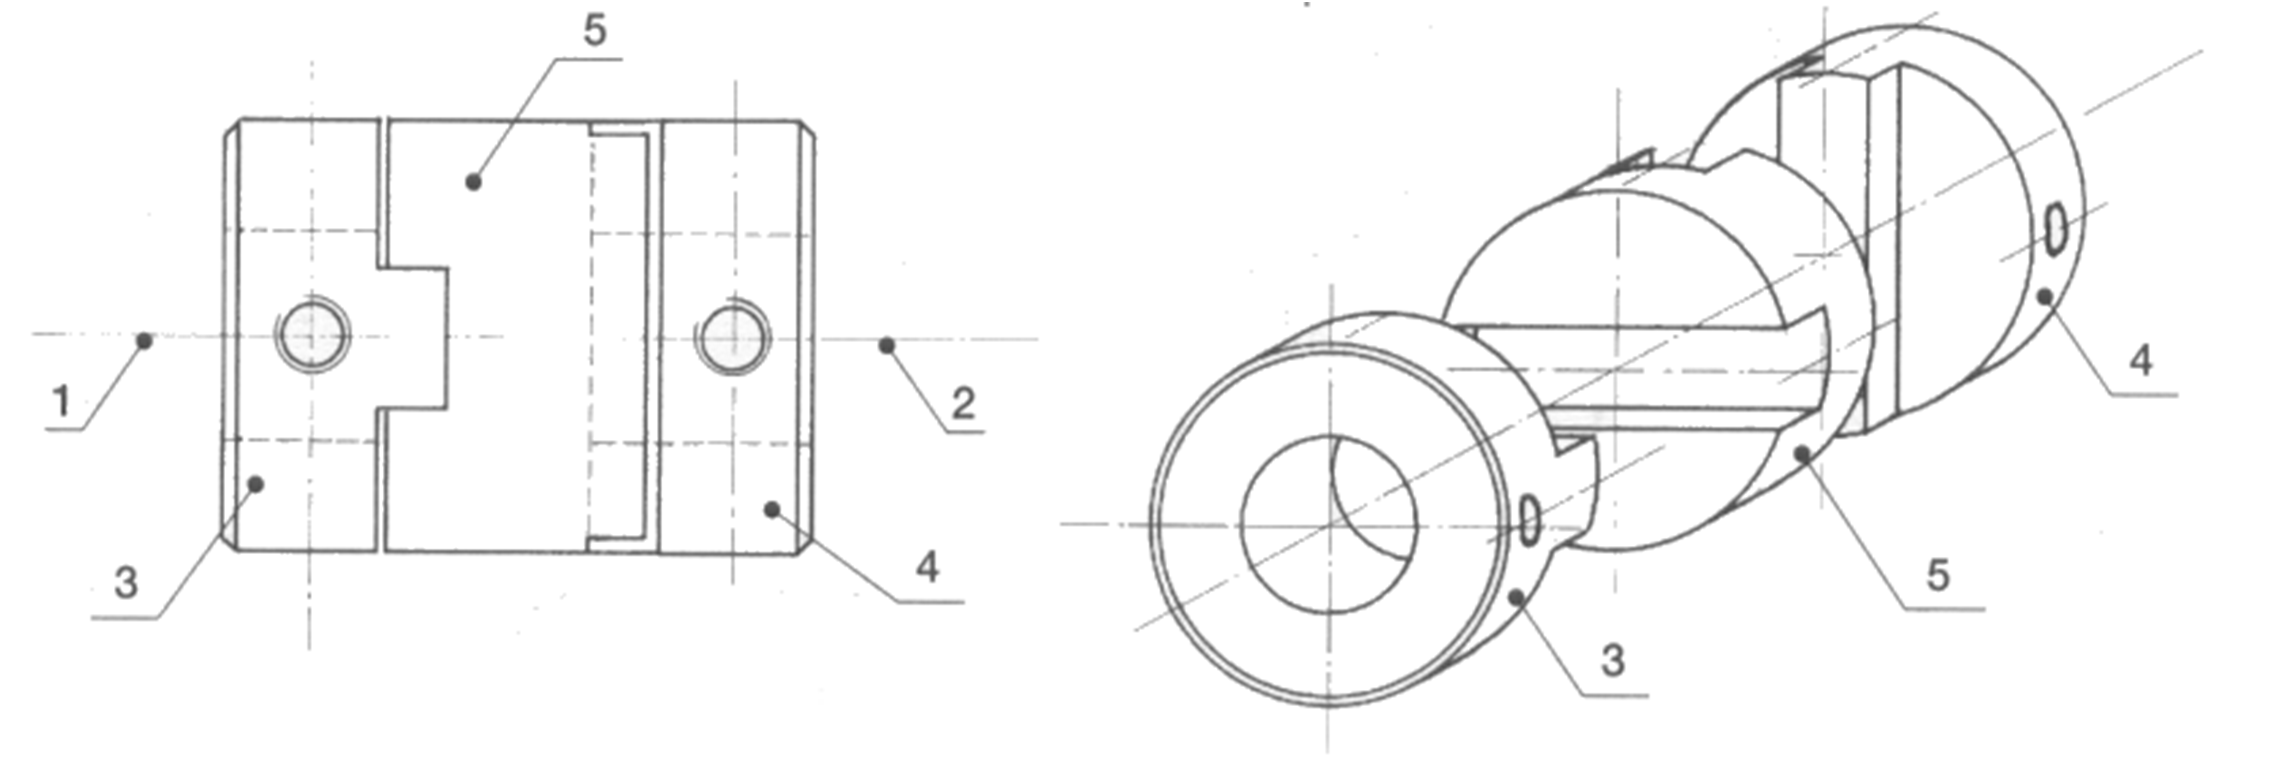
\includegraphics[height=4cm]{png/fig_18}
%\textit{}
\end{center}
\end{minipage}

Désalignement radial : 
$\Delta r = \pm 4\; mm$

Désalignement axial faible

Désalignement angulaire nul

Le joint de Oldham est homocinétique


\subsubsection{Les accouplements temporaires}
L’accouplement est dit temporaire lorsque les deux arbres peuvent être désolidarisés, sous l’action d’une commande extérieure (humaine ou automatisée).

\paragraph{Les roues libres}

La roue libre permet de transmettre la puissance entre deux arbres, mais uniquement pour un sens de rotation. C’est une transmission unidirectionnelle.


\begin{minipage}[c]{.2\linewidth}
\begin{center}
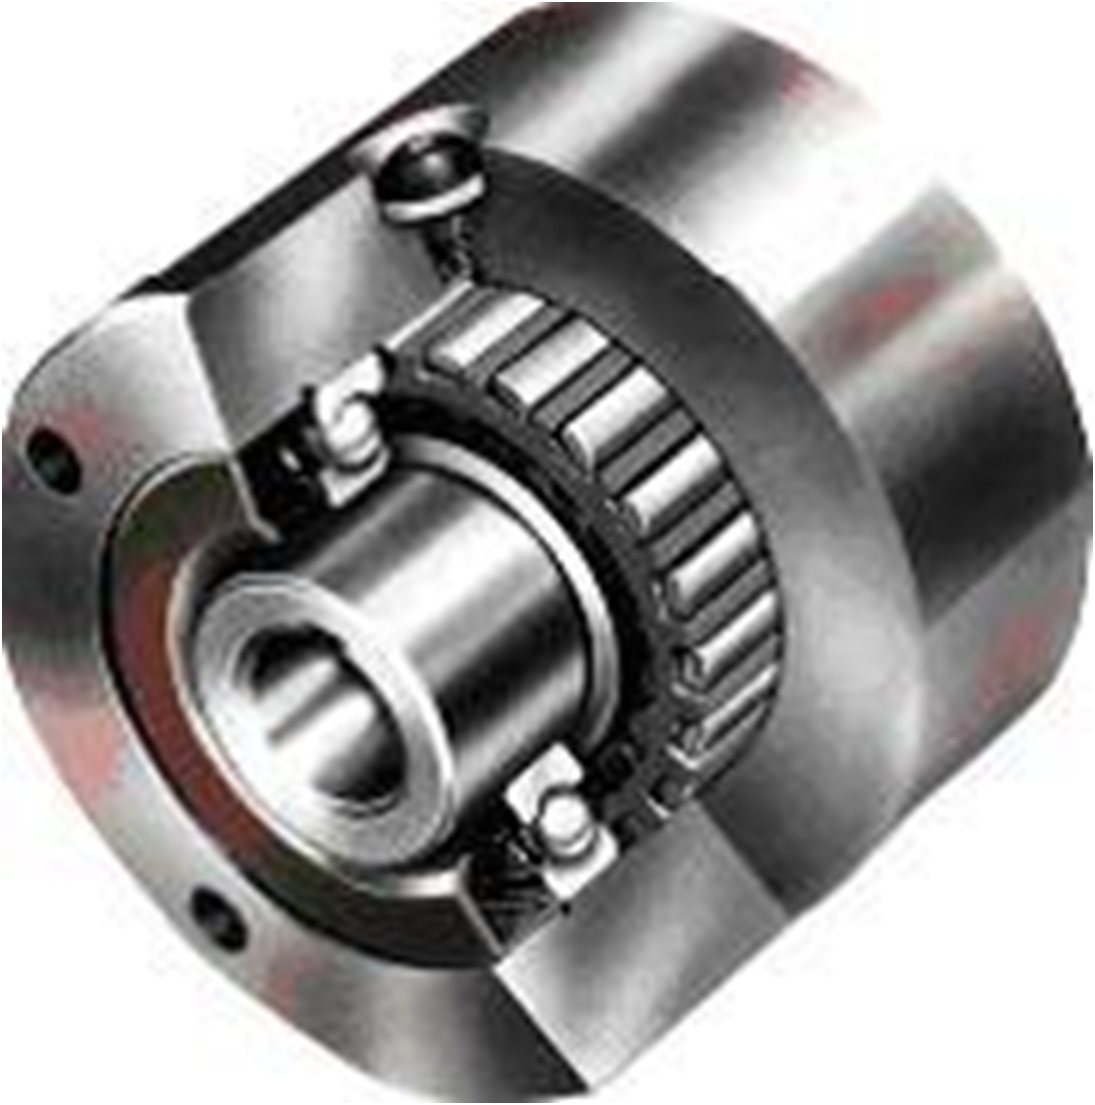
\includegraphics[height=3cm]{png/fig_19}

\textit{Avec rouleaux}
\end{center}
\end{minipage} \hfill
\begin{minipage}[c]{.2\linewidth}
\begin{center}
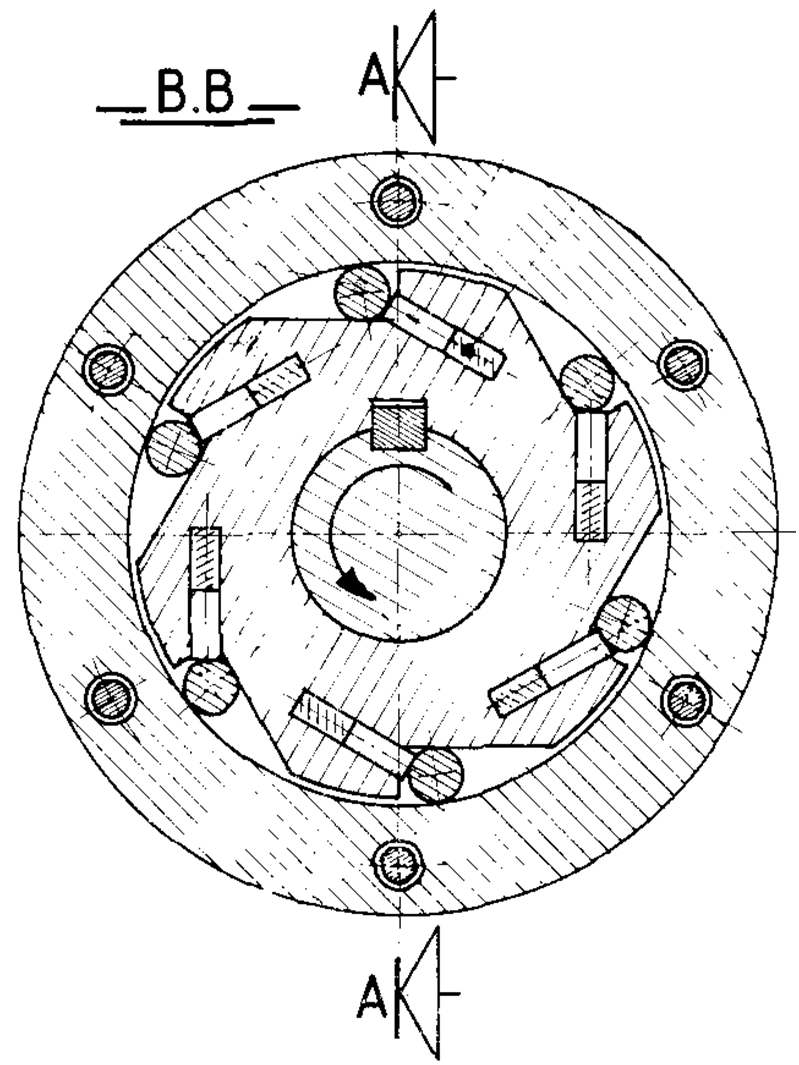
\includegraphics[height=4cm]{png/fig_20}

\textit{$\quad$}
\end{center}
\end{minipage} \hfill
\begin{minipage}[c]{.2\linewidth}
\begin{center}
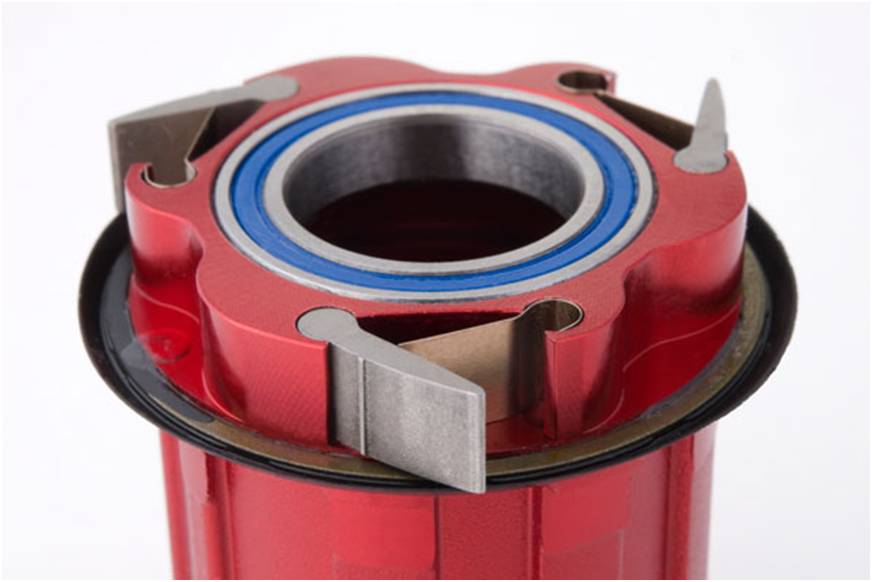
\includegraphics[height=3cm]{png/fig_21}
\textit{Avec cliquets}
\end{center}
\end{minipage} \hfill
\begin{minipage}[c]{.2\linewidth}
\begin{center}
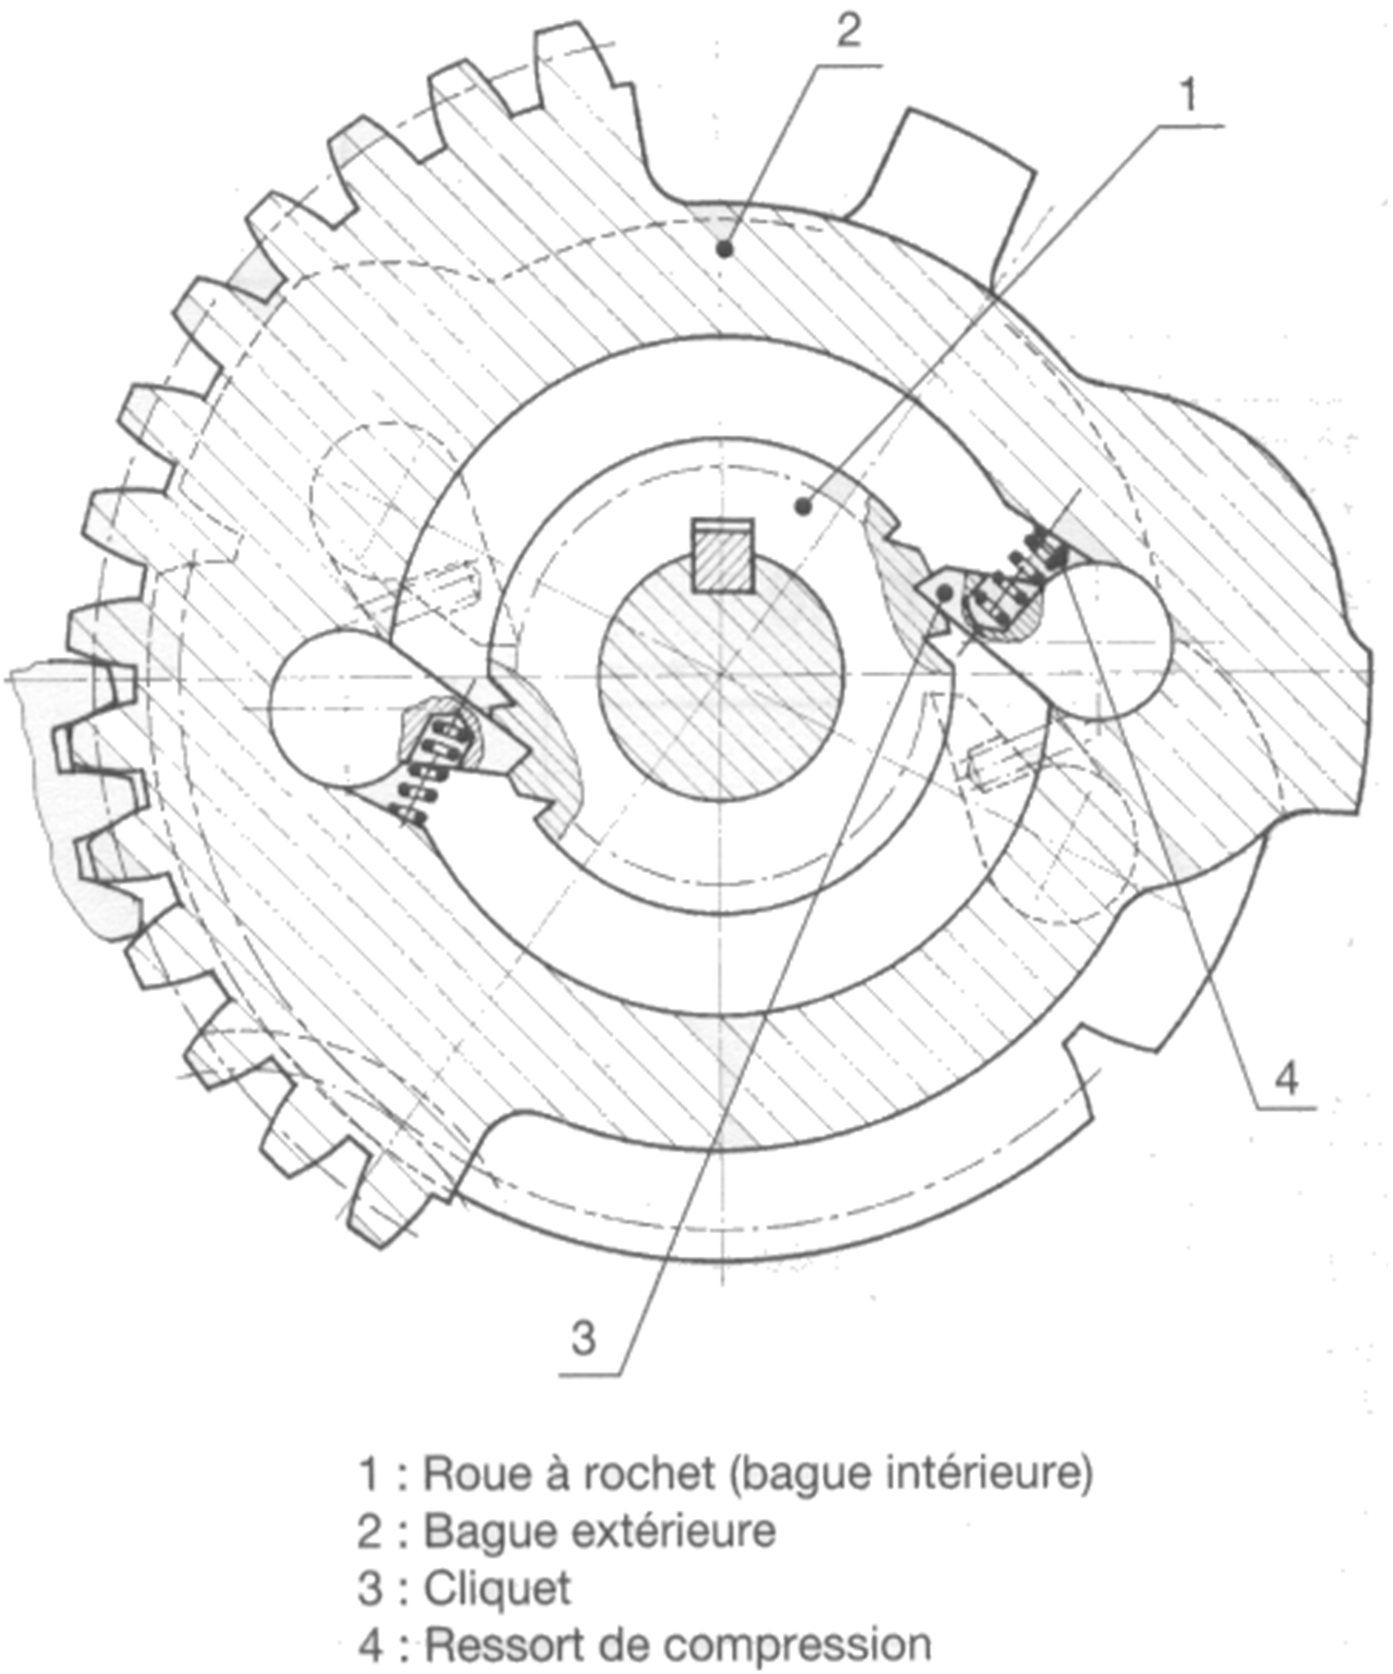
\includegraphics[height=4cm]{png/fig_22}

\textit{$\quad$}
\end{center}
\end{minipage} 

\paragraph{Les embrayages}

L’embrayage est un mécanisme qui permet d’accoupler ou de séparer, progressivement ou non, les arbres respectivement solidaires du moteur et du récepteur.

\begin{minipage}[c]{.45\linewidth}
\begin{center}
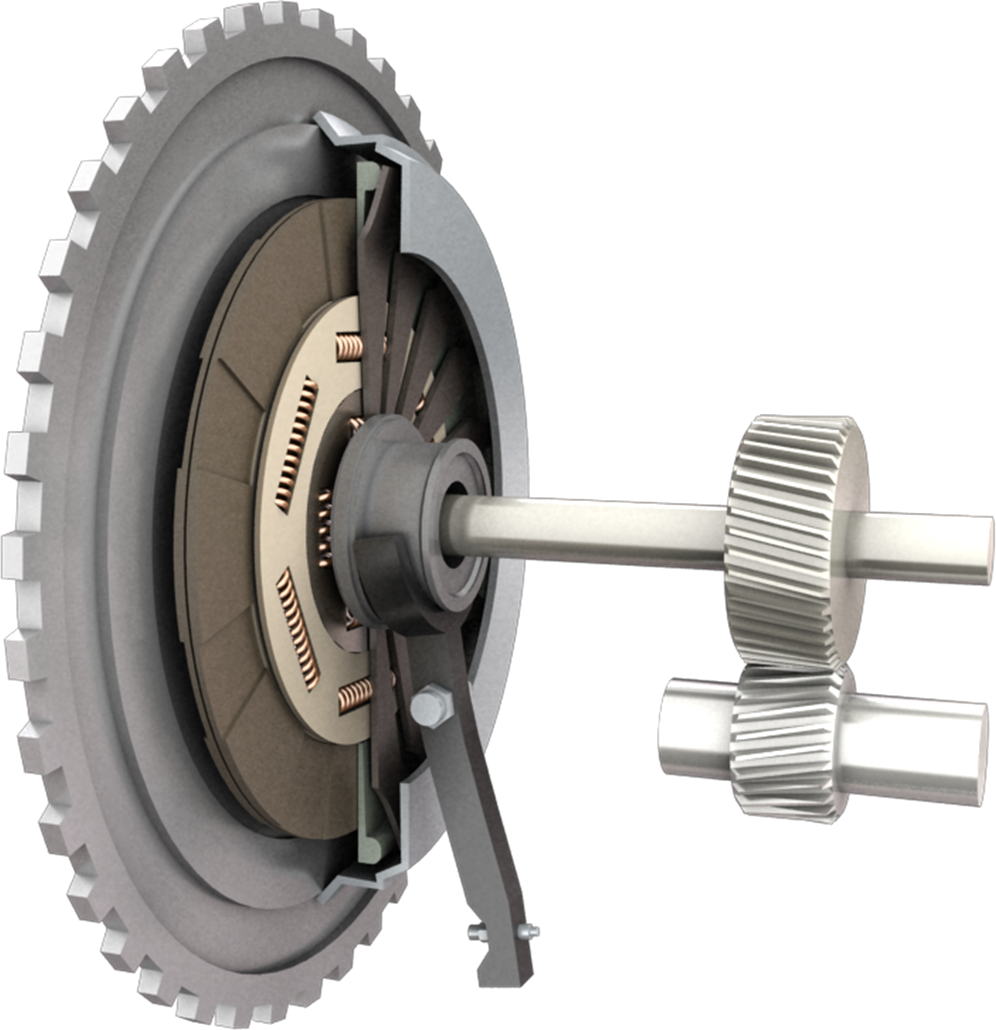
\includegraphics[height=5cm]{png/fig_23}
%\textit{Avec cliquets}
\end{center}
\end{minipage} \hfill
\begin{minipage}[c]{.45\linewidth}
\begin{center}
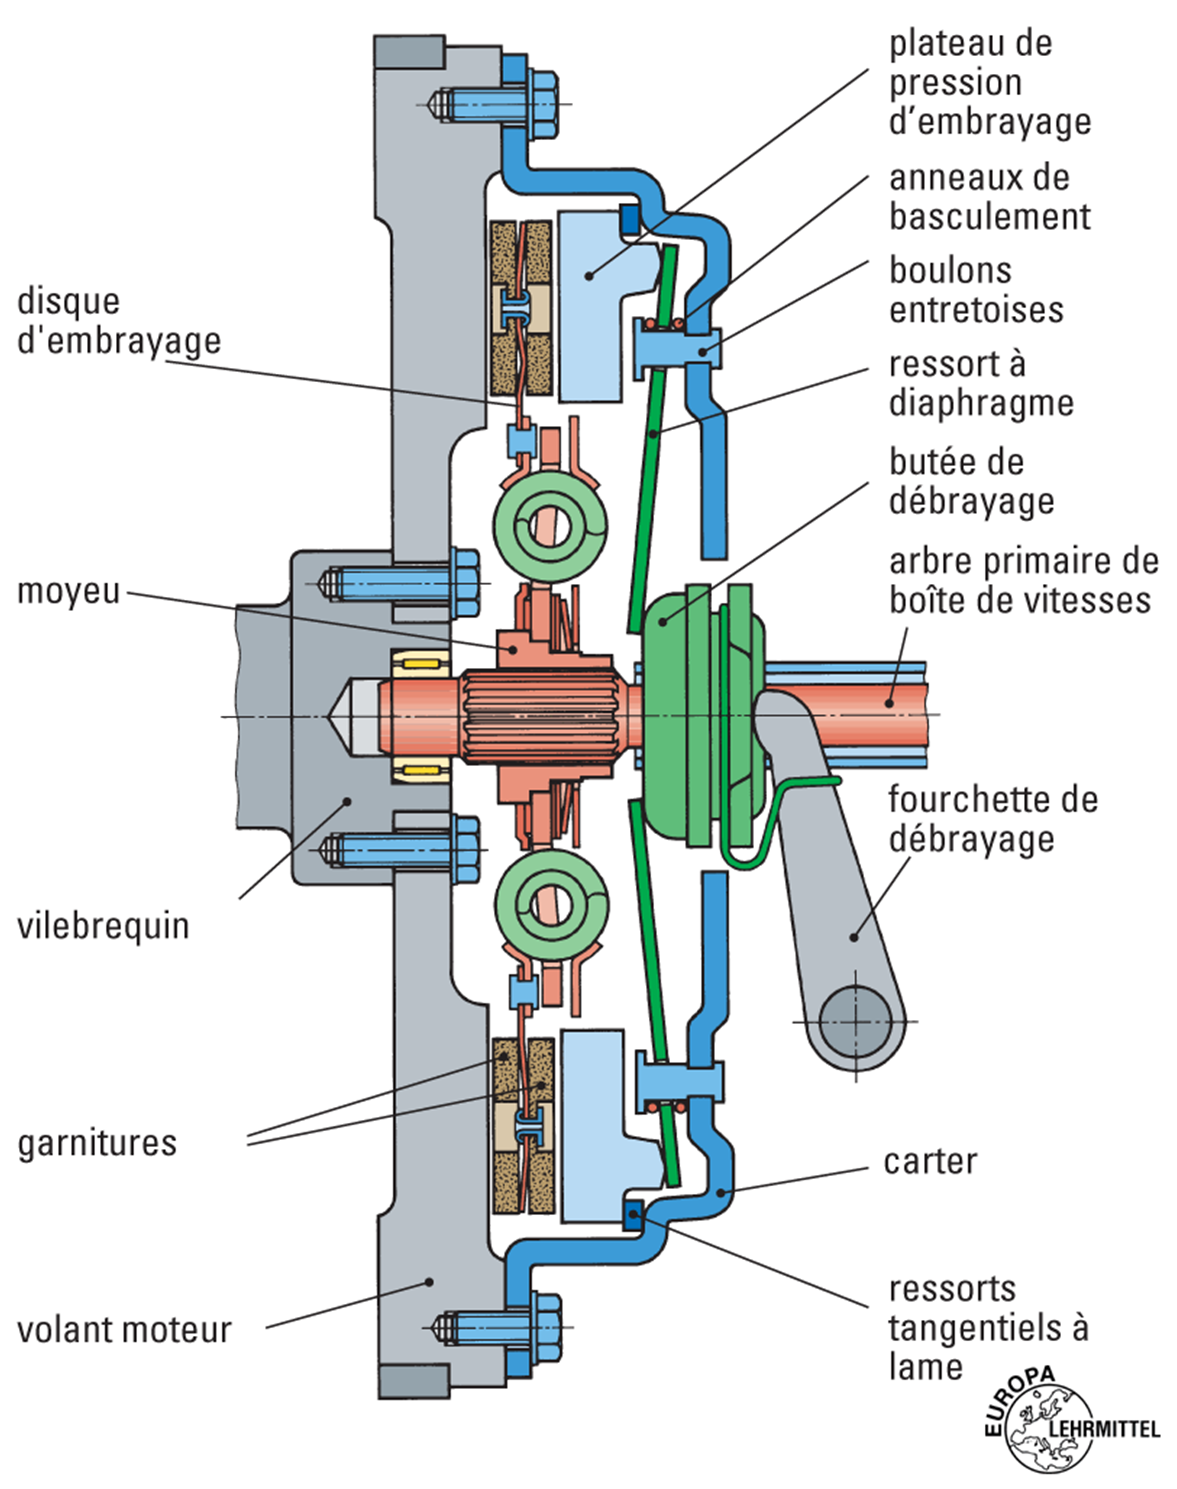
\includegraphics[height=8cm]{png/fig_24}
%\textit{}
\end{center}
\end{minipage}

\begin{center}
\textit{Embrayage à disque de friction et commande par fourchette}
\end{center}


Le couple transmissible par un embrayage à disques est donné dans le cas d’une modélisation à pression de contact uniforme par : 
$$
C_f = \dfrac{2}{3} n N f \dfrac{r_2^3-r_1^3}{r_2^2-r_1^2}
$$ 
où :
\begin{itemize}
\item $n$ : nombre de surfaces frottantes;
\item $N$ : effort presseur;
\item $f$ : facteur de frottement;
\item $r_2$ : grand rayon du disque;
\item $r_1$ : petit rayon du disque.
\end{itemize}
Formule approchée :  $C_f = 2nNfr_{moy}$  avec $r_{moy}$ rayon moyen.

\paragraph{Les coupleurs -- convertisseurs hydrodynamiques}

La transmission de l’énergie de l’arbre moteur vers l’arbre récepteur peut se faire par couplage hydraulique. 

Une roue à aubes « pompe » fournit l’énergie cinétique au fluide hydraulique. La roue à aubes « turbine » transforme cette énergie cinétique en énergie mécanique de rotation. Le couvercle assure l’étanchéité.
Il n’y a pas de liaison mécanique entre l’arbre d’entrée et l’arbre de sortie.

\begin{minipage}[c]{.45\linewidth}
\begin{center}
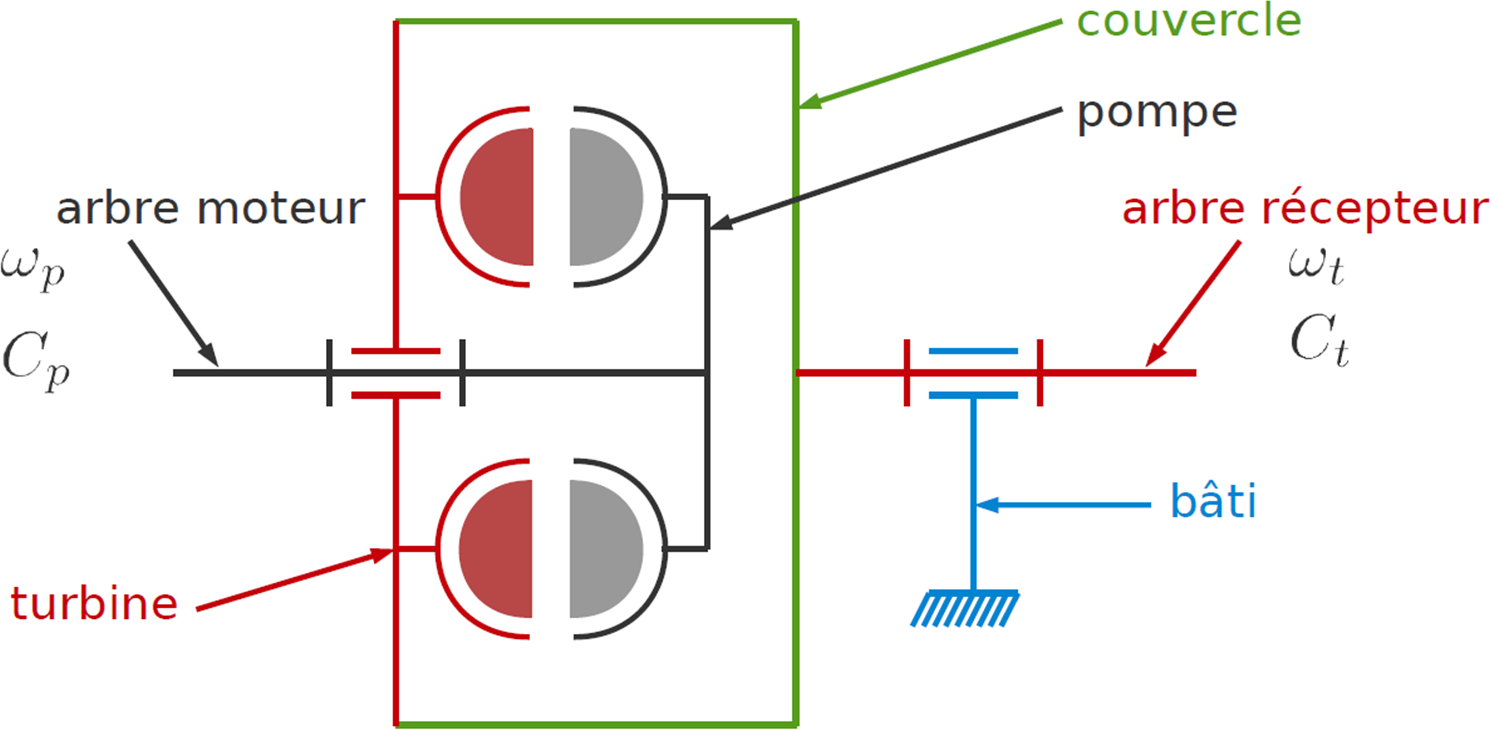
\includegraphics[height=4.5cm]{png/fig_25}
%\textit{Avec cliquets}
\end{center}
\end{minipage} \hfill
\begin{minipage}[c]{.45\linewidth}
\begin{center}
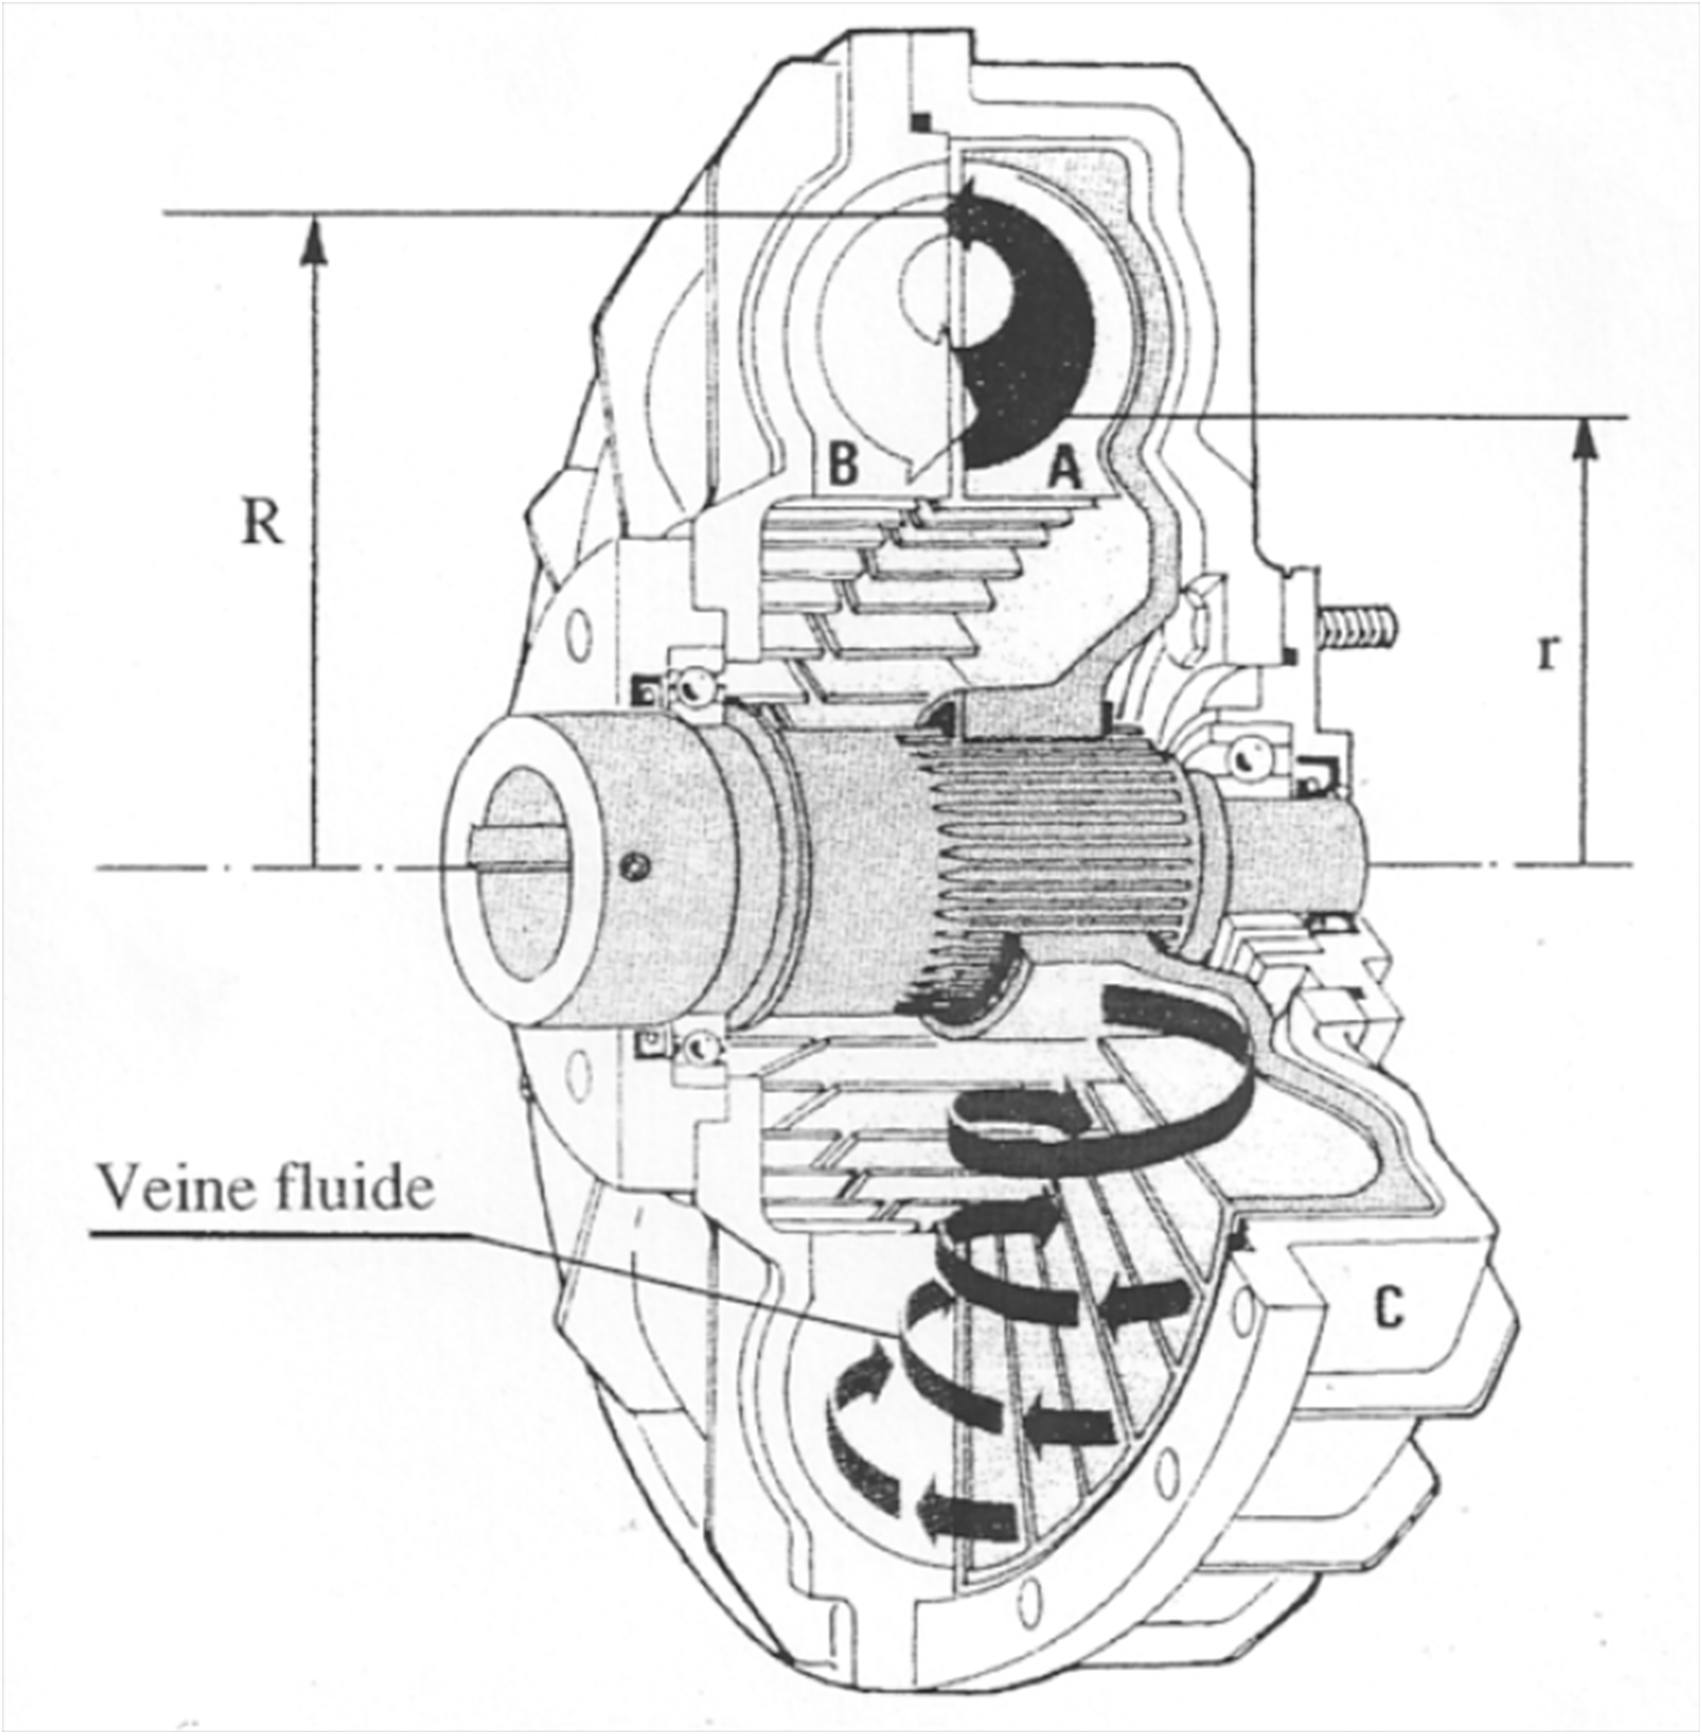
\includegraphics[height=5cm]{png/fig_26}
%\textit{}
\end{center}
\end{minipage}

Le coupleur filtre en partie les phénomènes vibratoires.

Afin de pouvoir faire varier le rapport de transmission, on rajoute une roue « réacteur ». Le coupleur est alors convertisseur. Sa structure est la suivante :

\begin{minipage}[c]{.45\linewidth}
\begin{center}
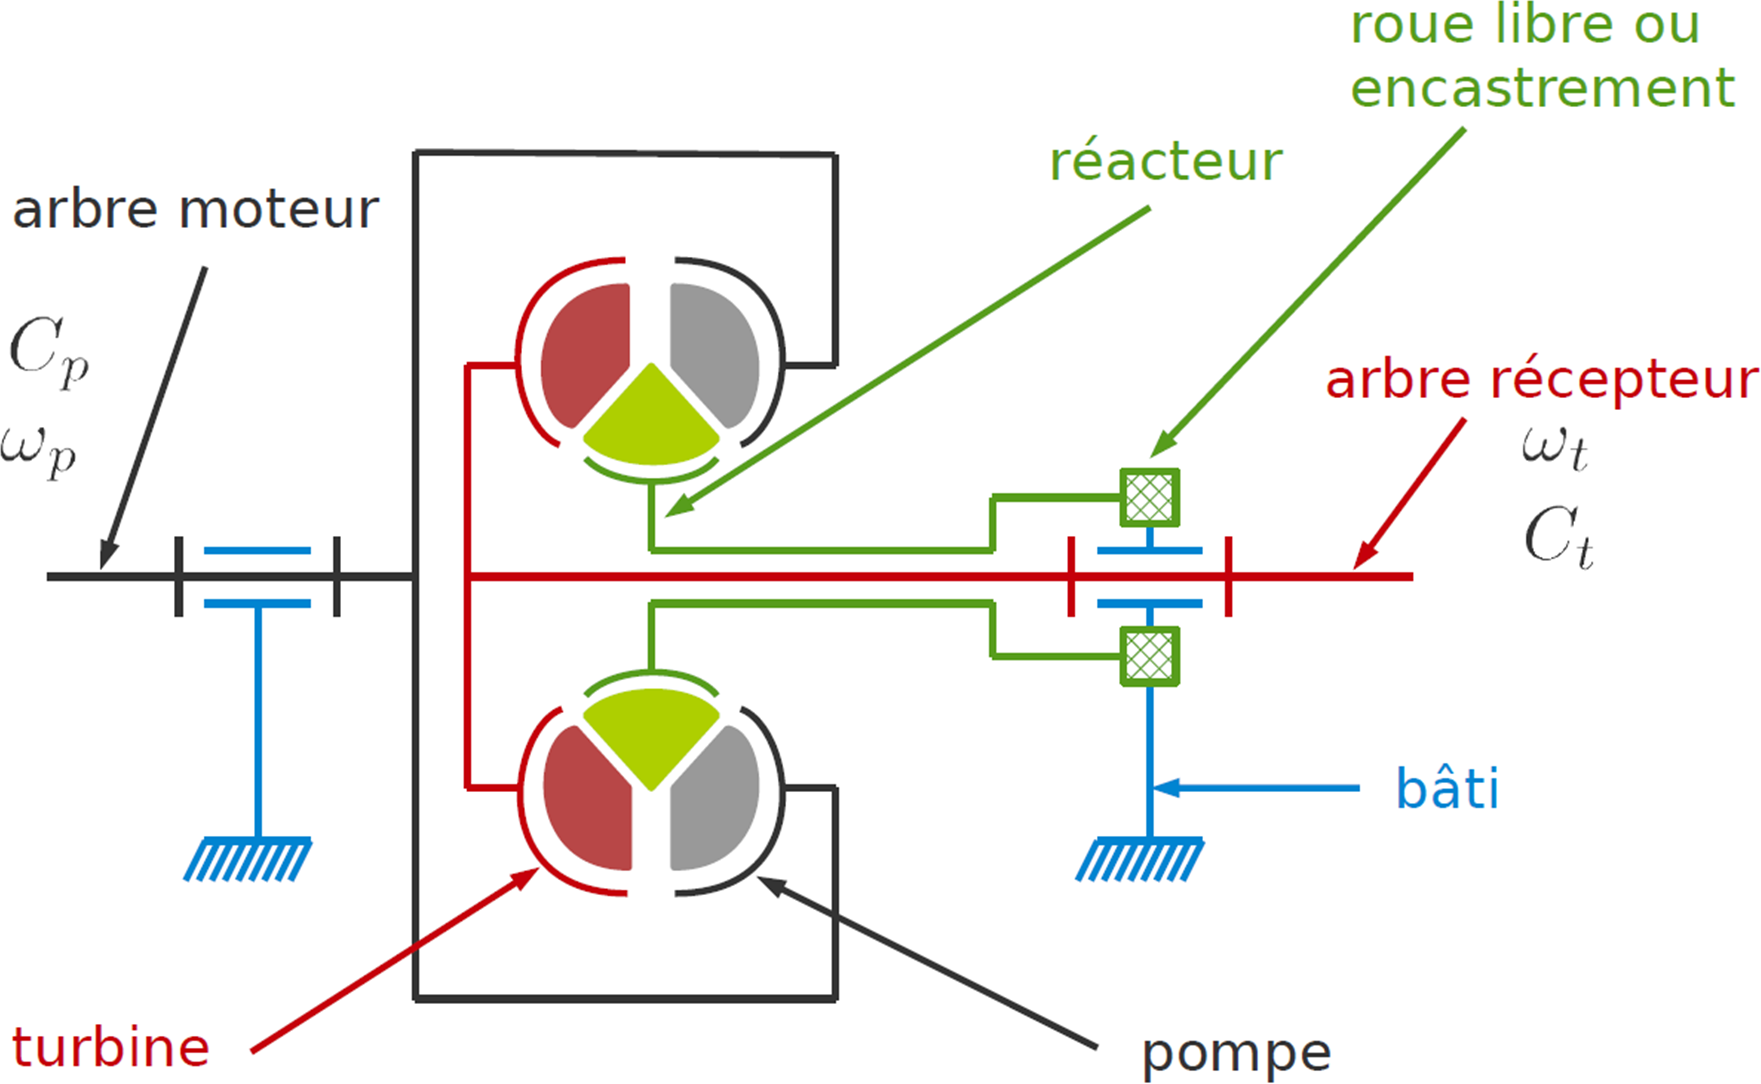
\includegraphics[height=4.5cm]{png/fig_27}
%\textit{Avec cliquets}
\end{center}
\end{minipage} \hfill
\begin{minipage}[c]{.45\linewidth}
\begin{center}
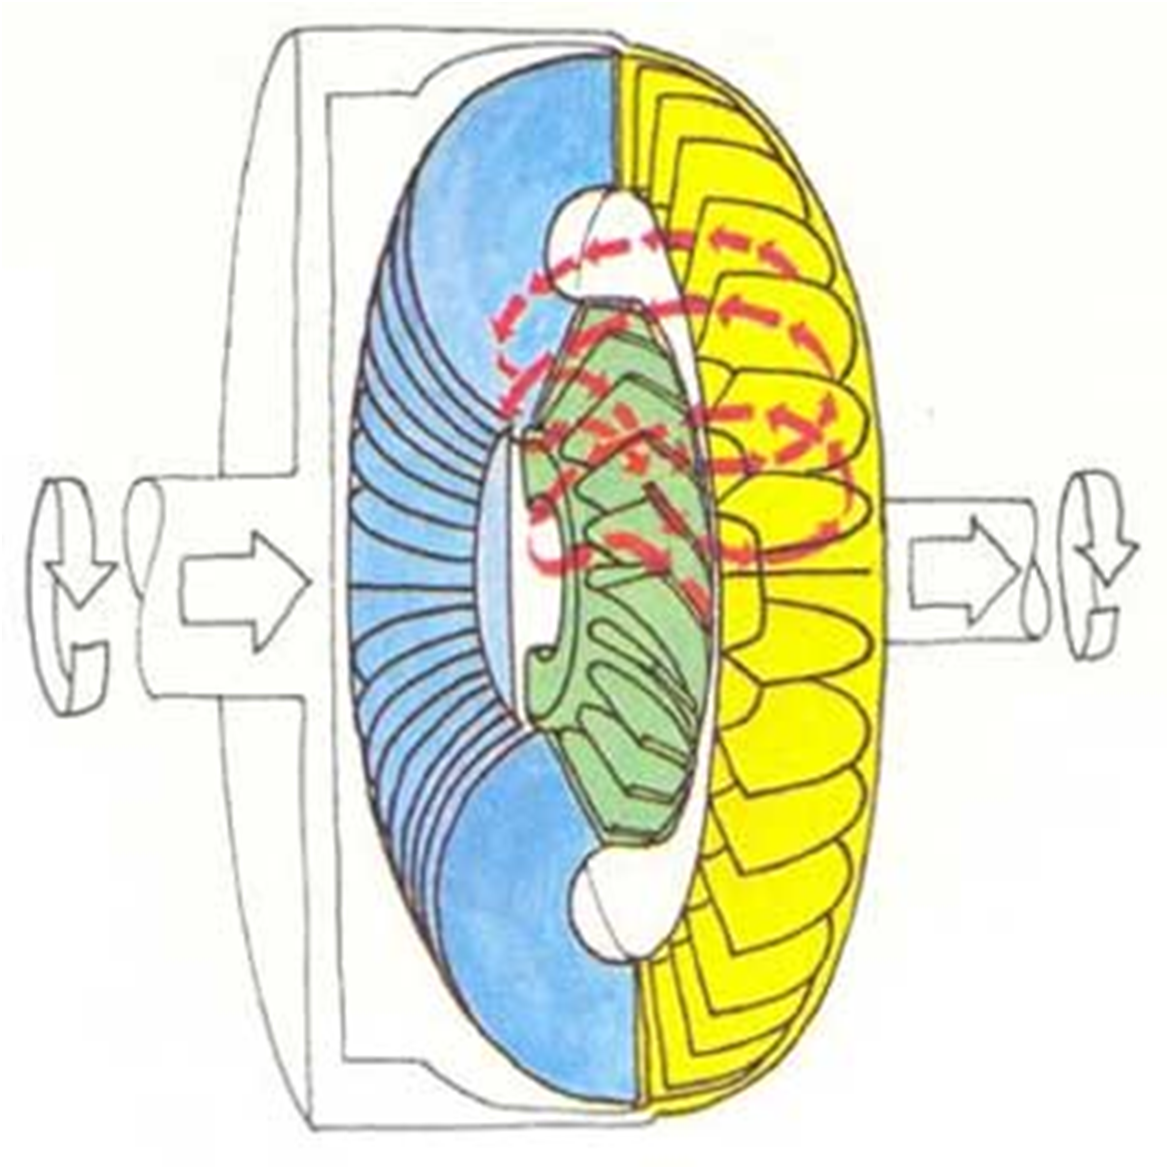
\includegraphics[height=5cm]{png/fig_28}
%\textit{}
\end{center}
\end{minipage}


\begin{minipage}[c]{.5\linewidth}
Le rendement d’un coupleur ( 97 \%) est meilleur que celui d’un convertisseur ( 85 \%). Dans le cas où il y a une roue libre, la roue « réacteur » est fixe jusqu’à ce que le couple exercé sur la roue « pompe » soit égal à celui exercé sur la roue « turbine ». Ensuite, on se retrouve donc dans la configuration d’un coupleur.

Il existe aussi des coupleurs / convertisseurs « lock-up » où un embrayage de pontage à friction solidarise la « pompe » et la « turbine » lorsque le convertisseur n’est pas nécessaire.


\end{minipage} \hfill
\begin{minipage}[c]{.45\linewidth}
\begin{center}
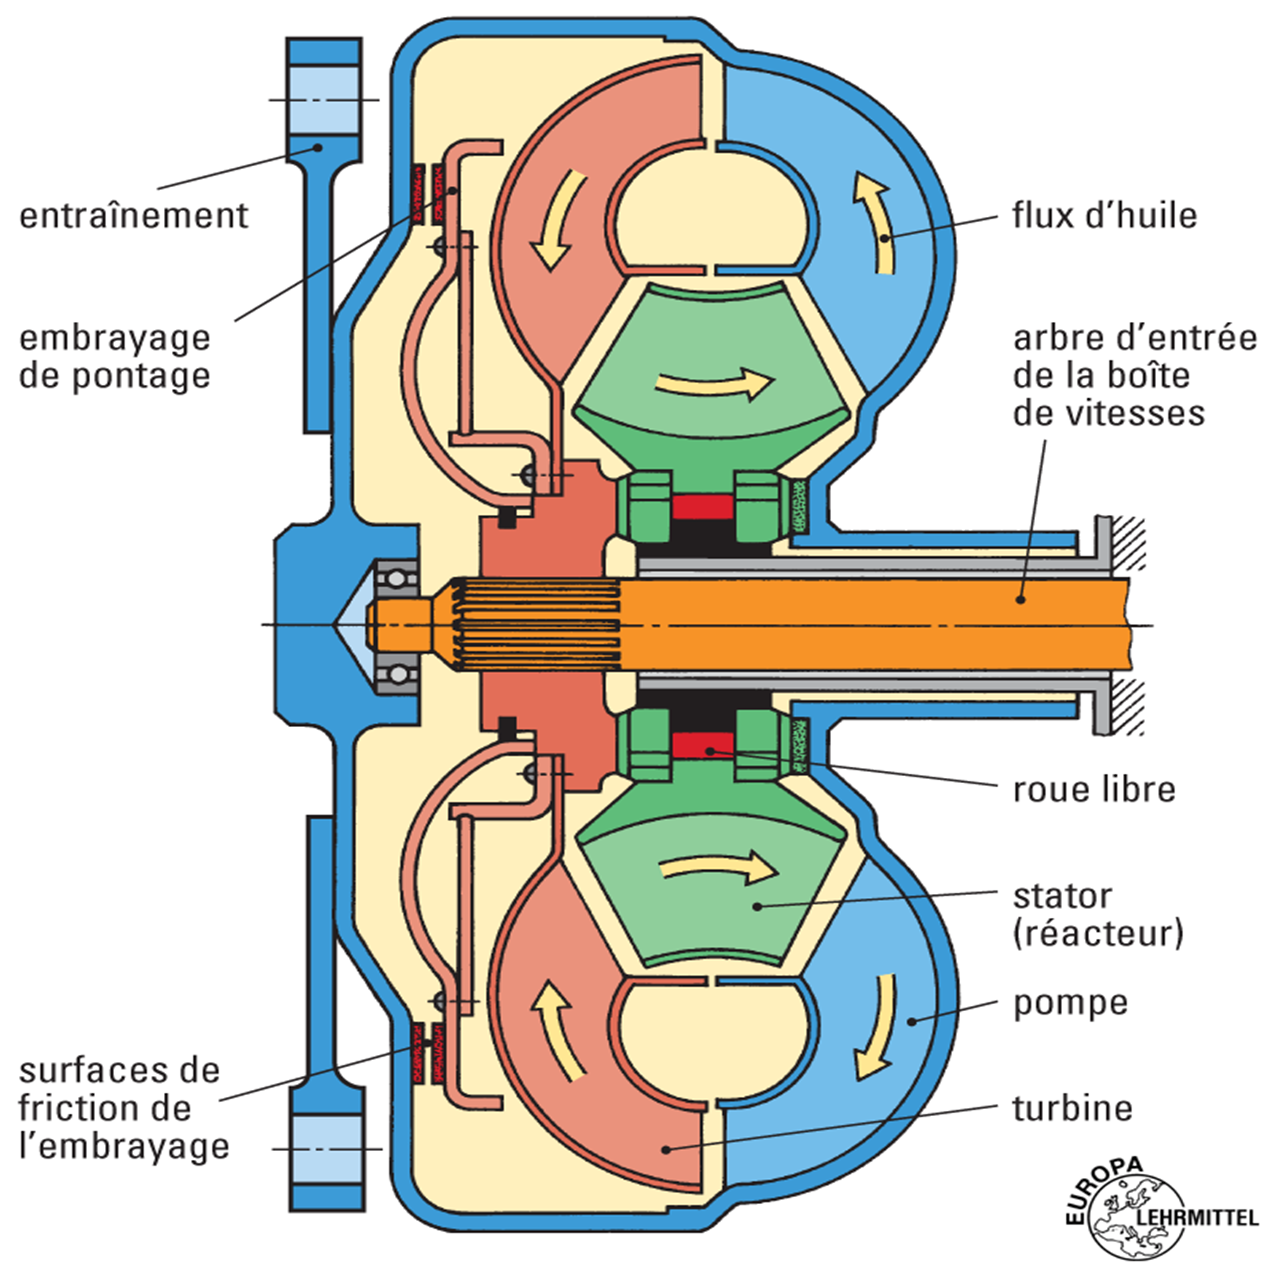
\includegraphics[height=6cm]{png/fig_29}
%\textit{}
\end{center}
\end{minipage}

\paragraph{Les limiteurs de couple}
Ce sont des organes de sécurité.

\begin{minipage}[c]{.3\linewidth}
\begin{center}
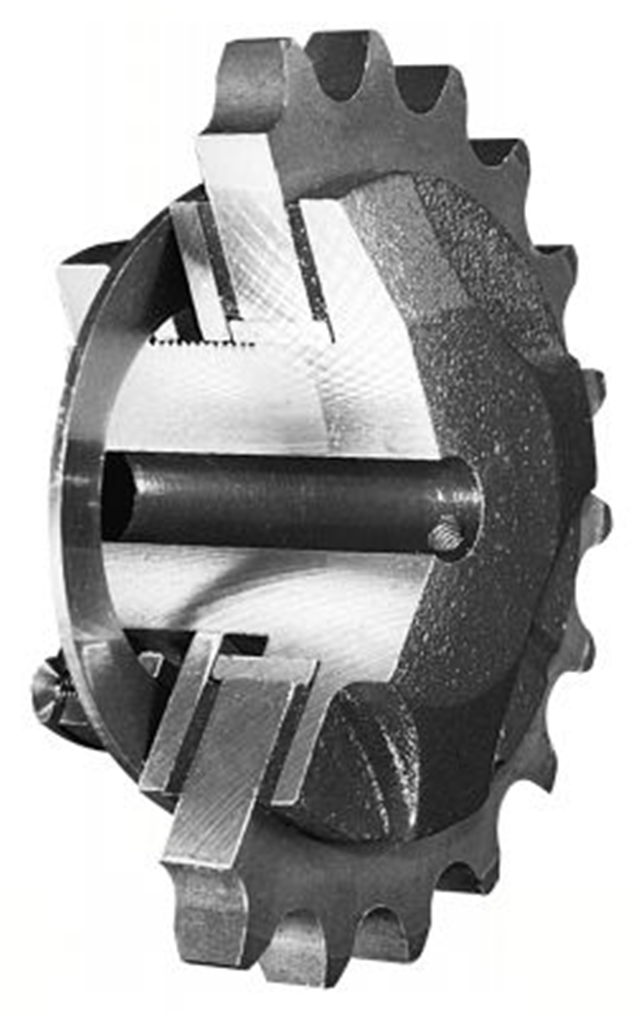
\includegraphics[height=5cm]{png/fig_30}

\textit{Avec glissement}
\end{center}
\end{minipage} \hfill
\begin{minipage}[c]{.3\linewidth}
\begin{center}
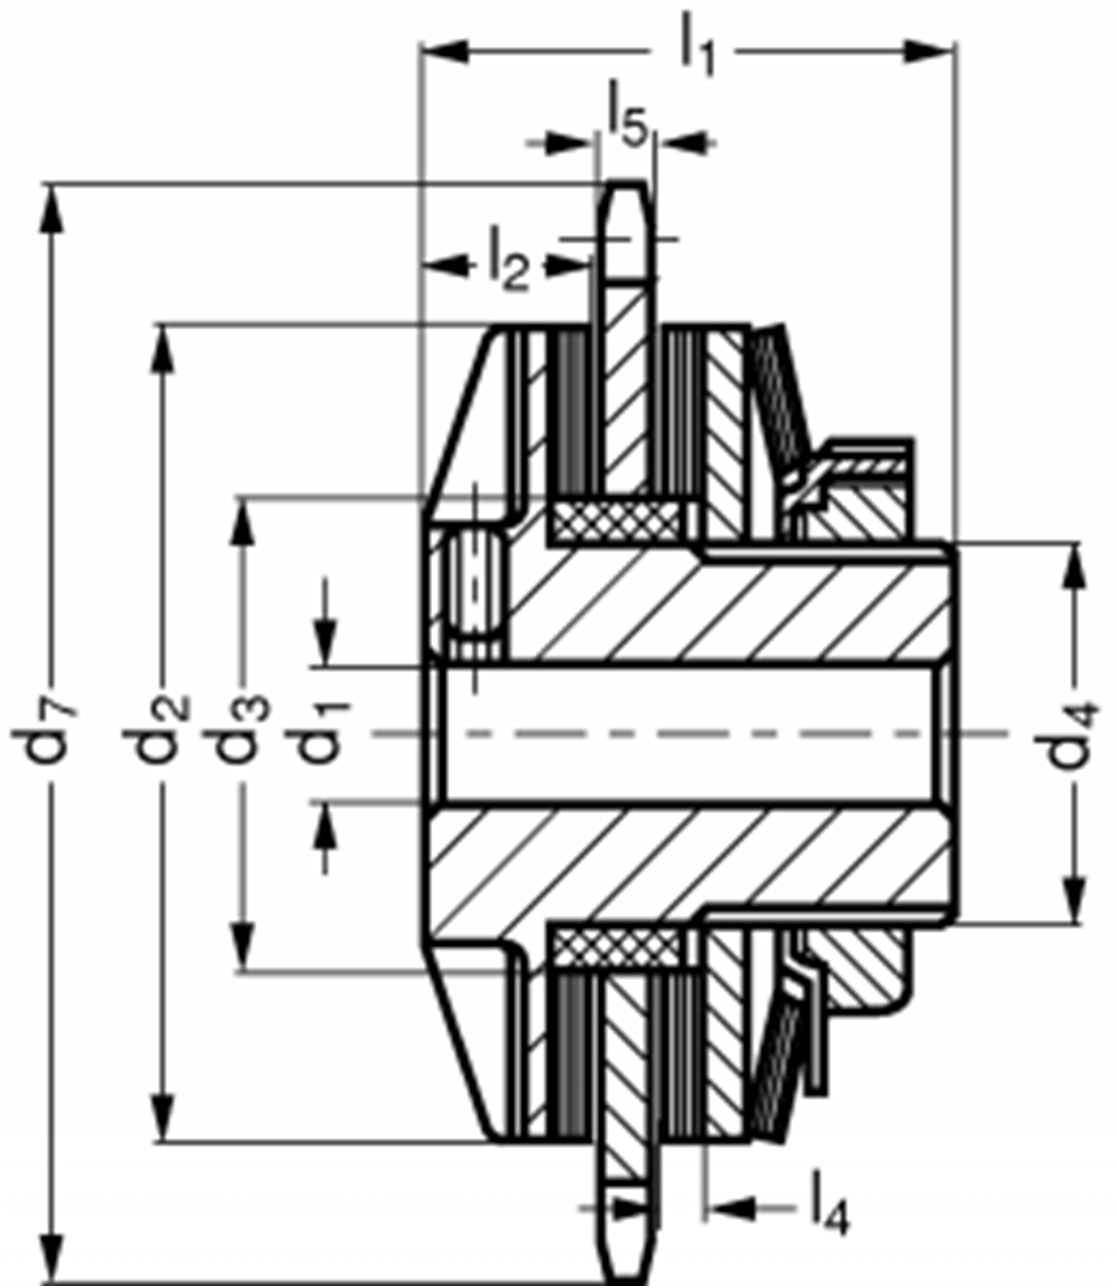
\includegraphics[height=5cm]{png/fig_31}

\textit{$\quad$}
\end{center}
\end{minipage}\hfill
\begin{minipage}[c]{.3\linewidth}
\begin{center}
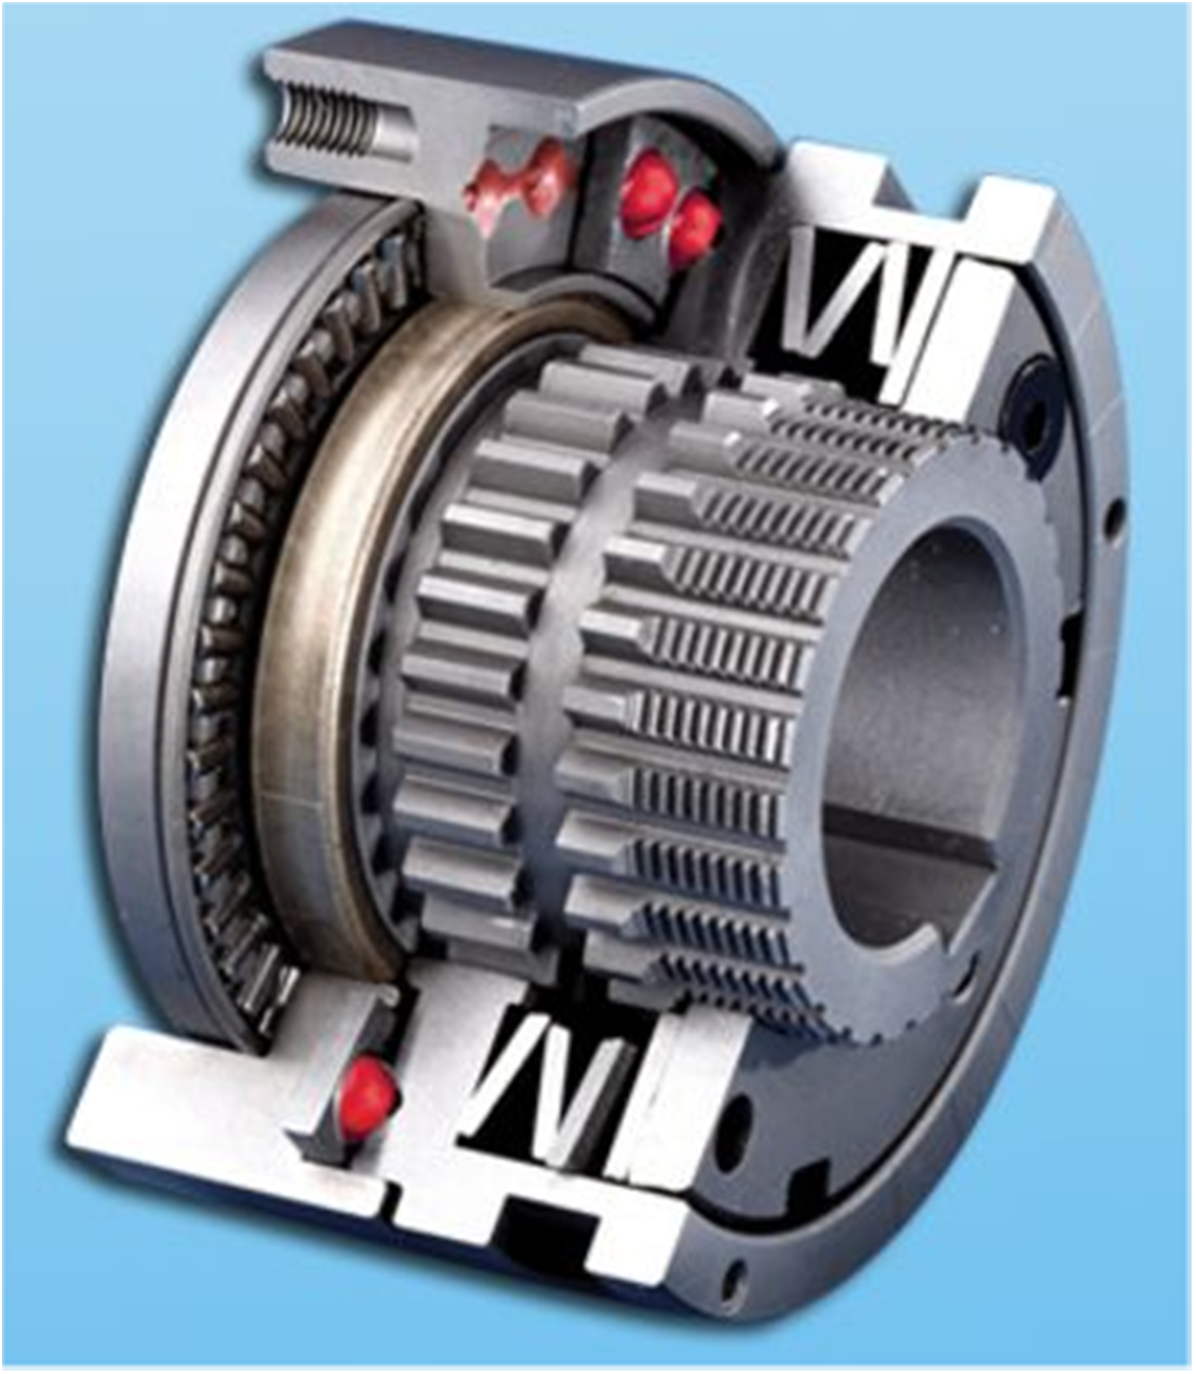
\includegraphics[height=5cm]{png/fig_32}

\textit{Avec obstacles (billes) }
\end{center}
\end{minipage}


\paragraph{Les freins}

Dans le cas des freins, la fonction est le plus souvent de ralentir ou d’arrêter l’arbre en mouvement. Beaucoup de systèmes de freinage existent : freins à tambours, à disques, à sabot, à sangle, etc.

\begin{center}
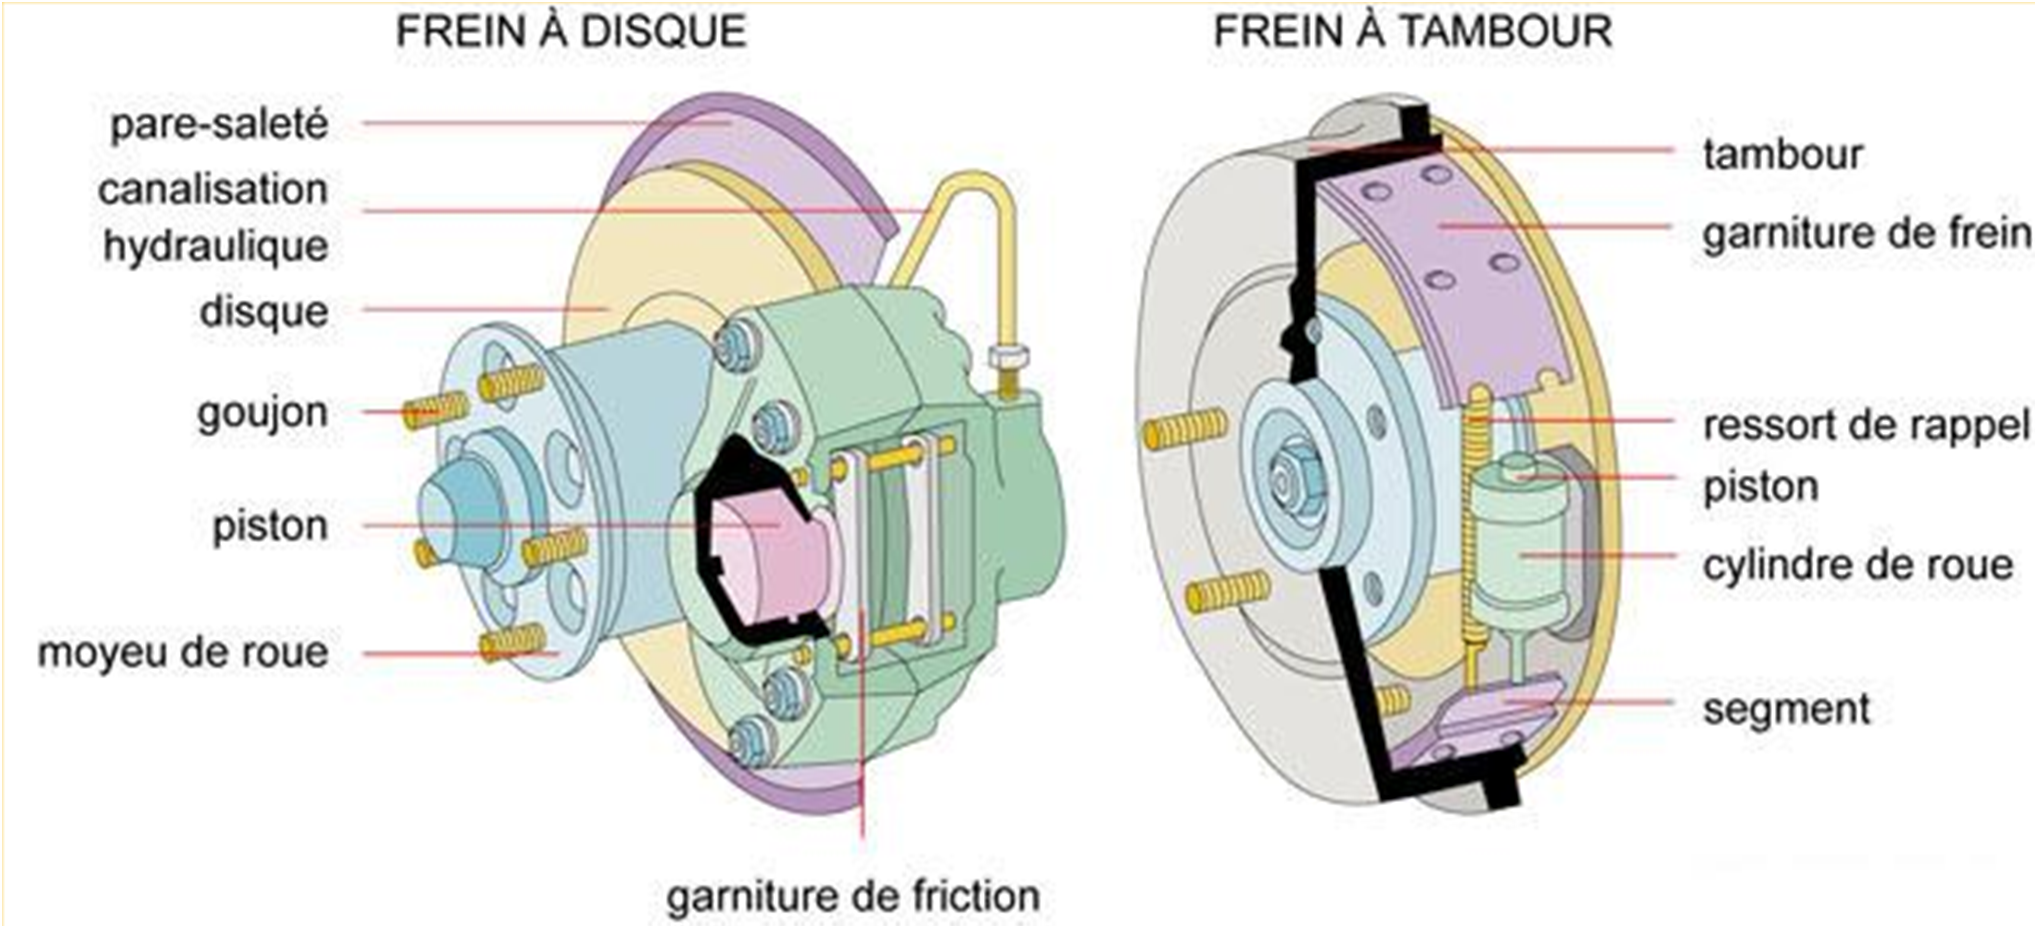
\includegraphics[height=6cm]{png/fig_33}
%\textit{Avec obstacles (billes) }
\end{center}



\subsection{Les accouplements entre arbres sécants}
Dans la chaîne de transmission de puissance, le joint d’accouplement entre arbres sécants doit réaliser une liaison de type sphérique à doigt :

\begin{minipage}[c]{.45\linewidth}
\begin{center}
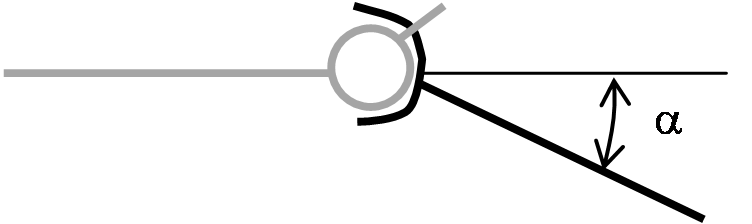
\includegraphics[width=\textwidth]{png/fig_34}
\end{center}
\end{minipage} \hfill
\begin{minipage}[c]{.45\linewidth}
$\alpha$ est appelé angle de brisure
\end{minipage}


Quelque soit l’angle de brisure, la puissance doit être transmise intégralement, au rendement près.
Ce joint d’accouplement trouve son utilité dans la propulsion marine (accouplement arbre moteur, arbre d’hélice), l’automobile (arbre de sortie du différentiel, arbre de roue motrice), les machines agricoles (prise de force, arbre d’entrée de diverses machines), etc.

Le joint d’accouplement est dit homocinétique, lorsqu’au cours du temps la vitesse de rotation de sortie, reste à tout instant égale à la vitesse de rotation d’entrée.

\subsubsection{Joints d’accouplement non homocinétiques -- le joint de cardan}
La liaison sphérique à doigt est réalisée à l’aide de deux liaisons pivots d’axes orthogonaux, en série.

\begin{center}
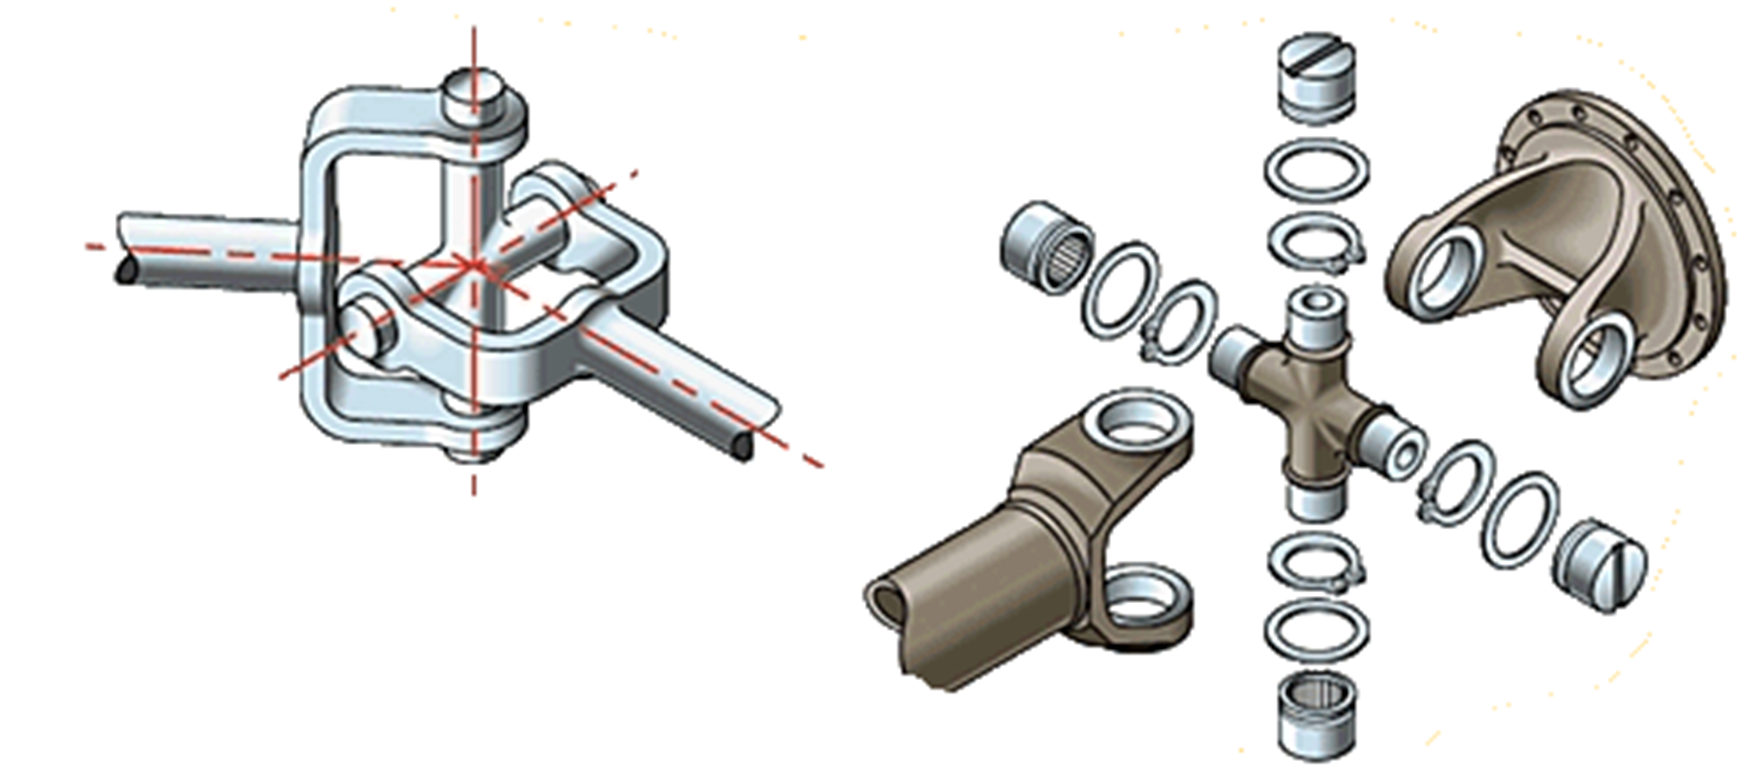
\includegraphics[height=5.5cm]{png/fig_35}
%\textit{Avec glissement}
\end{center}


La relation entre angle de sortie et angle d’entrée est : $\theta=arctan \left( \cos \alpha \cdot \tan \theta \right)$ . En pratique, l’angle de brisure est au maximum de 40 degrés.

\subsubsection{Joints d’accouplement homocinétiques}

\paragraph{Utilisation de deux cardans}
On peut réaliser un joint d’accouplement homocinétique avec deux cardans :

\begin{minipage}[c]{.6\linewidth}
\begin{center}
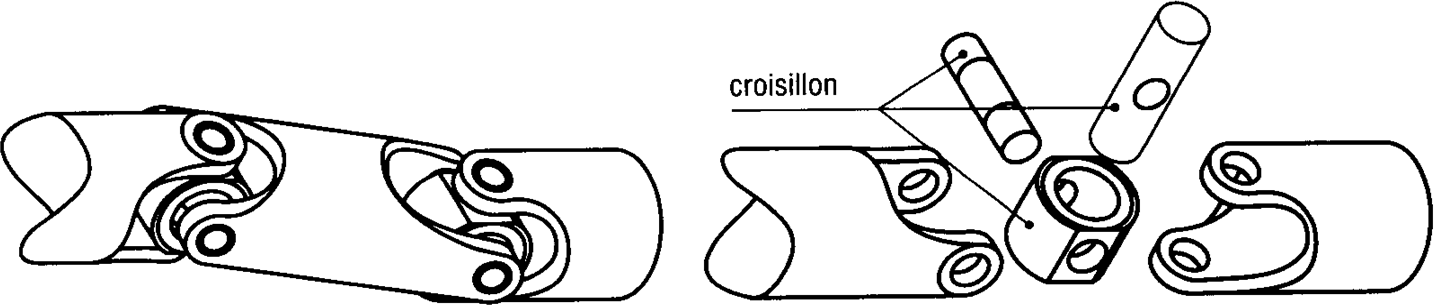
\includegraphics[width=.9\textwidth]{png/fig_36}
\end{center}
\end{minipage} \hfill
\begin{minipage}[c]{.3\linewidth}
\begin{center}
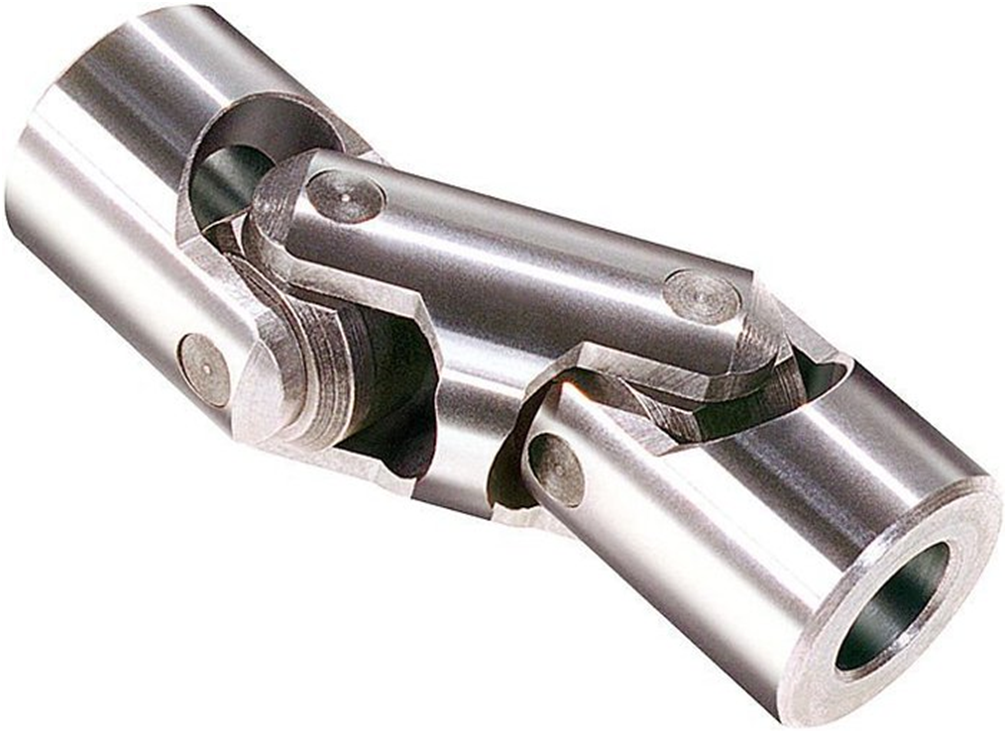
\includegraphics[width=.9\textwidth]{png/fig_36_b}
\end{center}
\end{minipage} 


\paragraph{Transmission automobile}


\begin{minipage}[c]{.5\linewidth}
\begin{center}
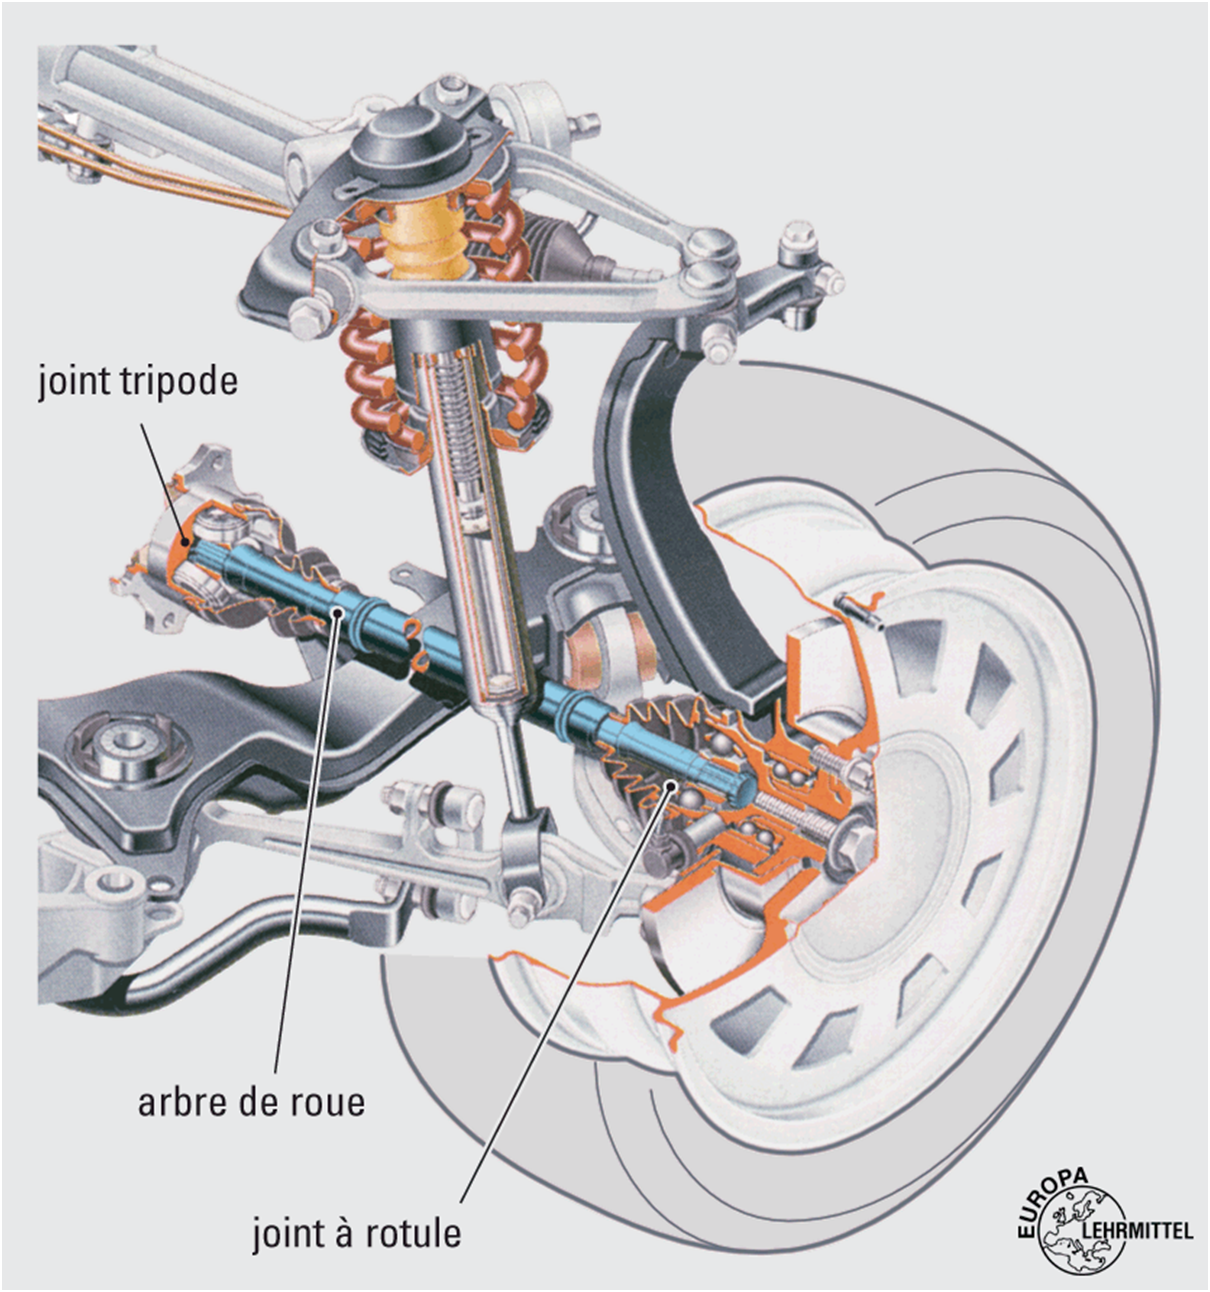
\includegraphics[width=.9\textwidth]{png/fig_37}
\end{center}
\end{minipage} \hfill
\begin{minipage}[c]{.45\linewidth}
\begin{center}
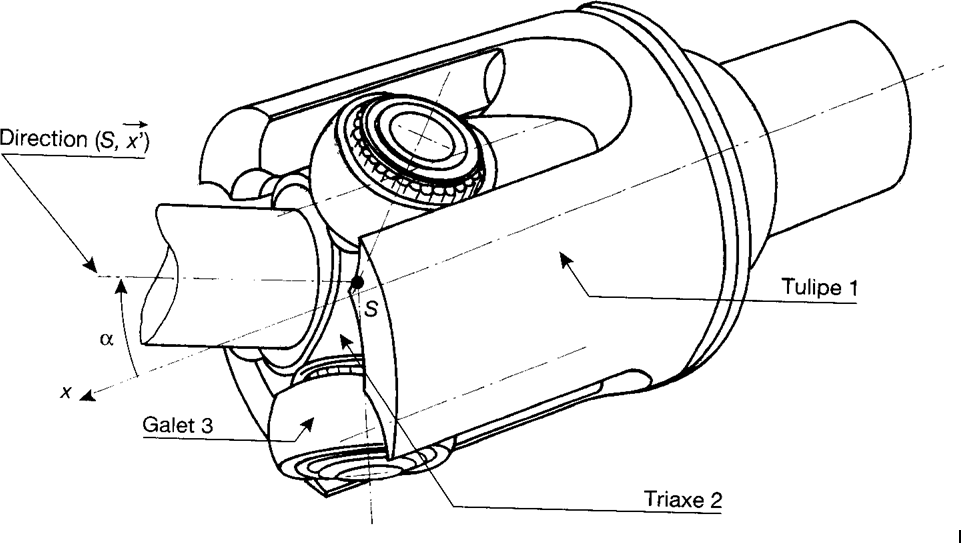
\includegraphics[height=3cm]{png/fig_38}

\textit{Joint tripode}

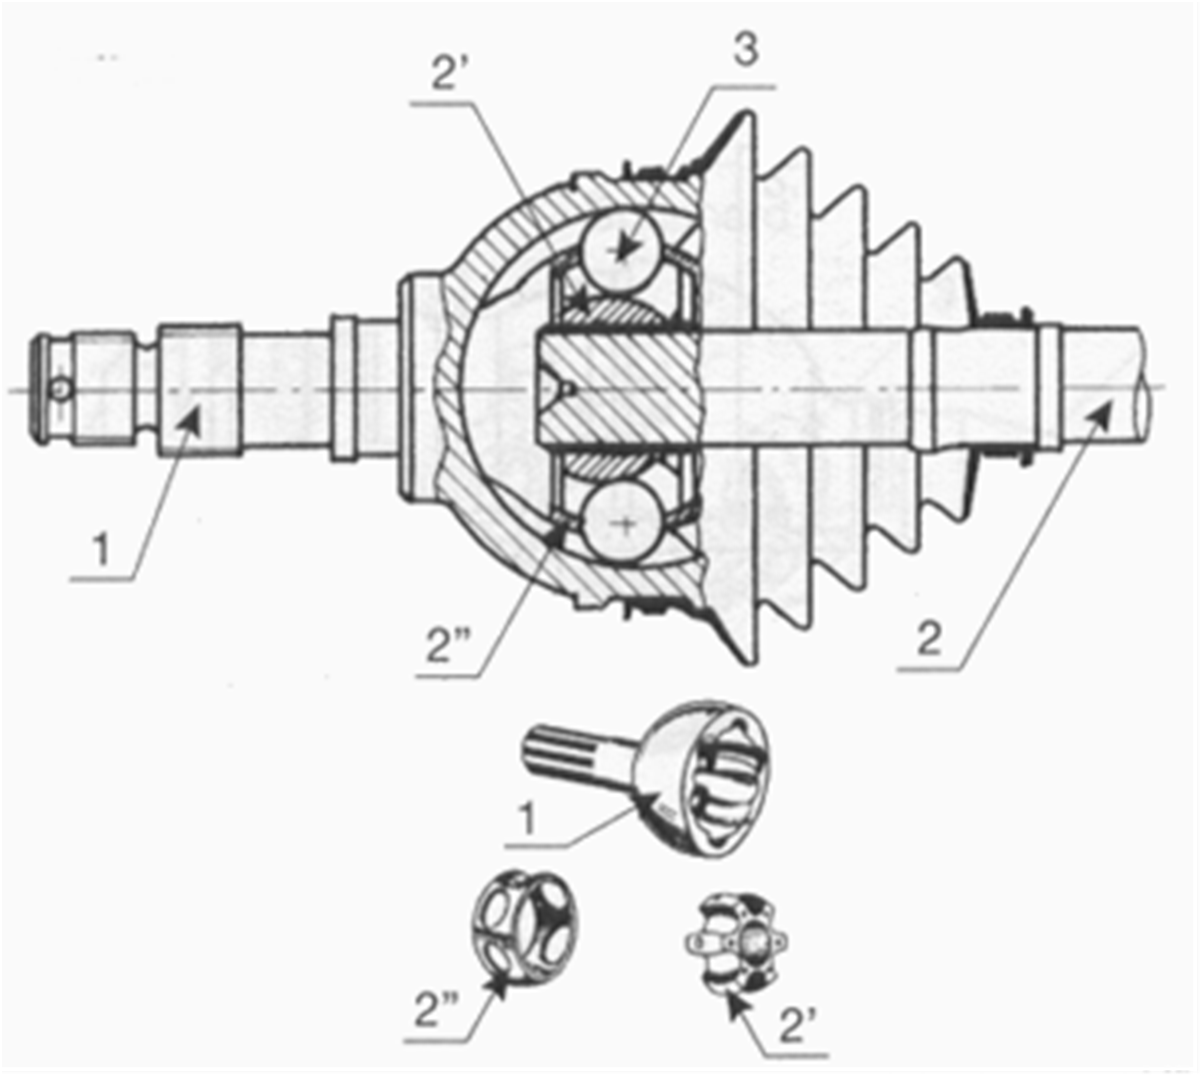
\includegraphics[height=5cm]{png/fig_39}

\textit{Joint à rotule Rzeppa}

\end{center}
\end{minipage} 


\section{La transmission de l’énergie sans transformation de mouvement et avec modification de la vitesse de rotation}
\subsection{Mise en situation}

Les réducteurs et multiplicateurs sont des transmetteurs de puissance.

Leur place dans la chaîne d’énergie est la suivante :
\begin{center}
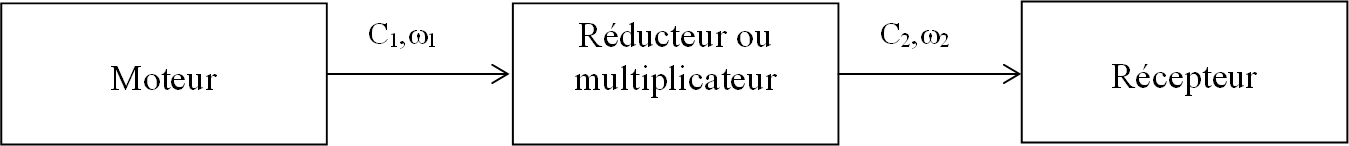
\includegraphics[width=.8\textwidth]{png/fig_40}
\end{center}

\subsubsection{Aspect cinématique}
Lorsque l’on a $\left|\dfrac{\omega_2}{\omega_1} \right|<1$ , on parle de réducteur. Lorsque l’on a $\left|\dfrac{\omega_2}{\omega_1} \right|>1$, on parle de multiplicateur.

On parle aussi d’inverseur lorsqu’il y a inversion du sens de rotation.

On appelle rapport de transmission ou rapport de réduction le rapport $\dfrac{\omega_1}{\omega_2}$ .

Le rapport de multiplication est l’inverse du rapport de transmission.

Dans une boîte de vitesse d’automobile, on peut passer par tous ces états. L’utilisation d’un réducteur ou d’un multiplicateur peut permettre d’adapter la fréquence de rotation, à la nécessité d’une fonction. Par exemple, en fabrication, afin d’imposer une vitesse de coupe spécifique selon les matériaux utilisés pour l’outil et la pièce à usiner, il est nécessaire de pouvoir régler la fréquence de rotation de la broche. Selon l’application, le rapport des fréquences de rotation peut soit être fixe, soit être variable (variateur, boîte de vitesse).


\subsubsection{Aspect énergétique}
Si le rendement du réducteur ou du multiplicateur est idéal, on a la conservation de la puissance mécanique : $C_1 \cdot \omega_1 = C_2 \cdot \omega_2$ . On en déduit alors : $\dfrac{C_2}{C_1}=\dfrac{\omega_1}{\omega_2}$.

Dans le cas d’un réducteur de fréquence de rotation, il y a multiplication du couple.

Dans le cas d’un multiplicateur de fréquence de rotation, il y a réduction du couple.

Si l’on prend en compte le rendement de la transmission $\eta$, on a  $C_1 \cdot \omega_1 \cdot \eta = C_2 \cdot \omega_2$.

\subsection{La transmission de puissance par courroie}


Une courroie est un lien flexible destiné à assurer une transmission de puissance entre un arbre moteur et un arbre récepteur,  dont les axes sont en général parallèles. Pour le montage le plus courant, il n’y a pas d’inversion de sens de rotation.

\begin{minipage}[c]{.55\linewidth}
La transmission par poulie / courroie asynchrone, présente les avantages suivant :
\begin{itemize}
\item arbres d’entrée et de sortie éloignés ;
\item possibilité de variation d’entraxe ;
\item souplesse de la transmission ;
\item pas de lubrification ;
\item fonctionnement silencieux ;
\item bon rendement (>95 \%) ;
\item coût réduit.
\end{itemize}
\end{minipage} \hfill
\begin{minipage}[c]{.4\linewidth}
\begin{center}
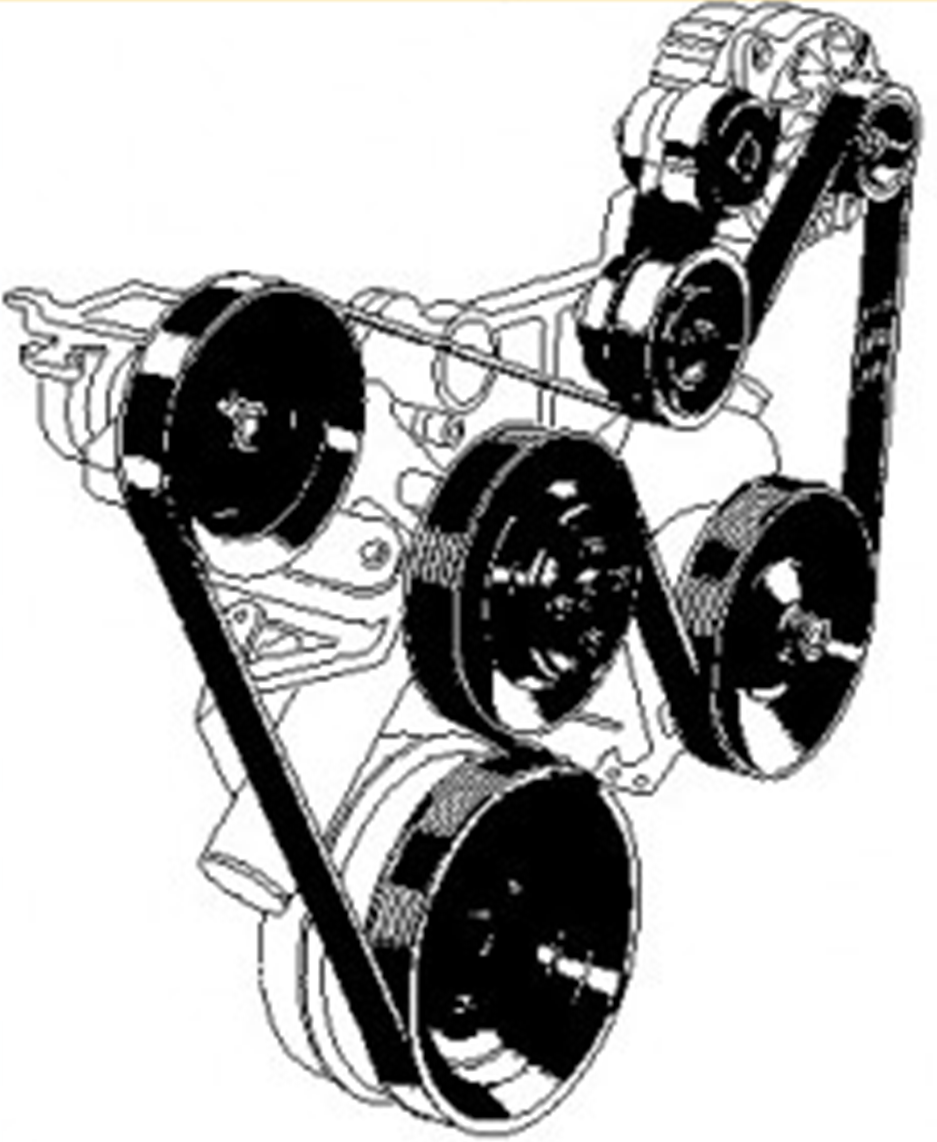
\includegraphics[height=5cm]{png/fig_41}
\end{center}
\end{minipage} 

Les inconvénients de ce type de transmission sont principalement :
\begin{itemize}
\item transmission non homocinétique (glissement pour courroie non synchrone);
\item efforts radiaux important (tension de pose nécessaire).
\end{itemize}
\subsubsection{Comportement cinématique}

\begin{minipage}[c]{.55\linewidth}
\begin{center}
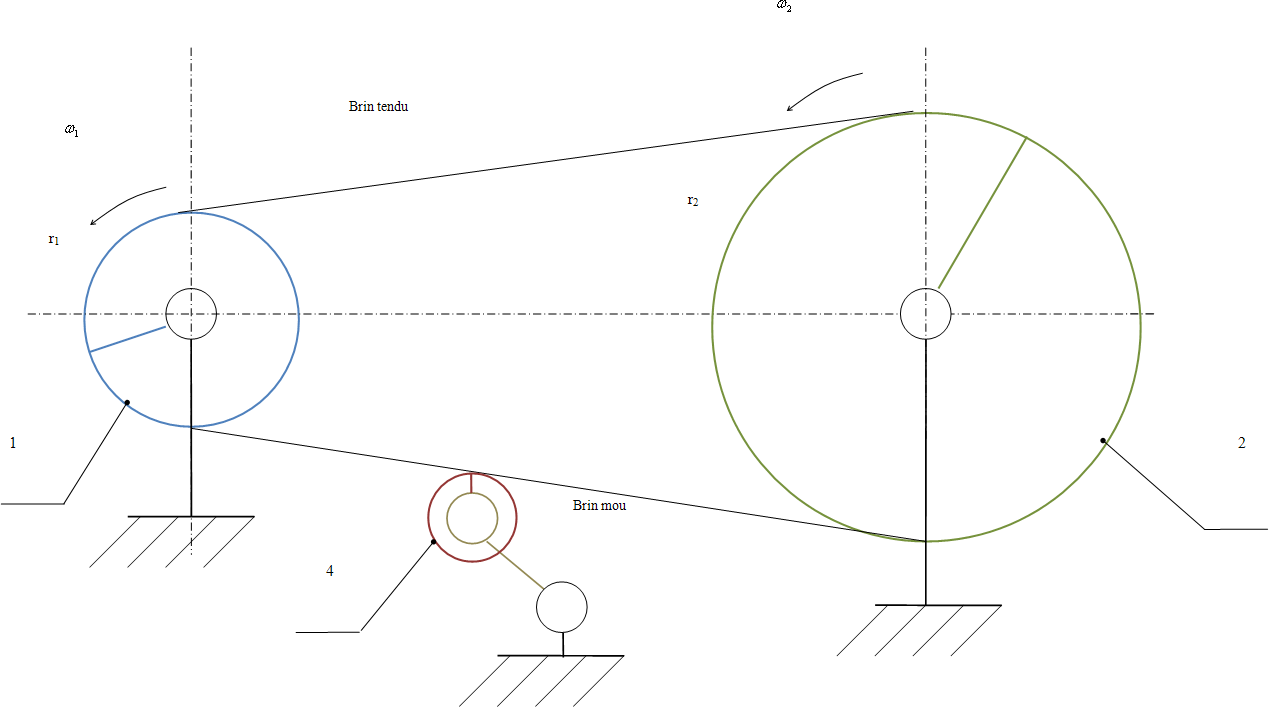
\includegraphics[width=.9\textwidth]{png/fig_42}
\end{center}
\end{minipage} \hfill
\begin{minipage}[c]{.4\linewidth}
\begin{enumerate}
\item 1 : poulie motrice, rayon $r_1$ ;
\item 2 : poulie réceptrice, rayon $r_2$ ;
\item 4 : galet tendeur.
\end{enumerate}
\end{minipage} 

Dans le cas où il y a non glissement,  $\dfrac{\omega_2}{\omega_1} = \dfrac{r_1}{r_2} $.
Dans la réalité, il y peut y avoir glissement de la courroie sur la poulie. Ce glissement fonctionnel noté $g$, est de l’ordre de 2\% en général. On a alors $\dfrac{\omega_2}{\omega_1}=\left(1-g\right) \dfrac{r_1}{r_2}$.

\subsubsection{Longueur de courroie}


\begin{minipage}[c]{.55\linewidth}
\begin{center}
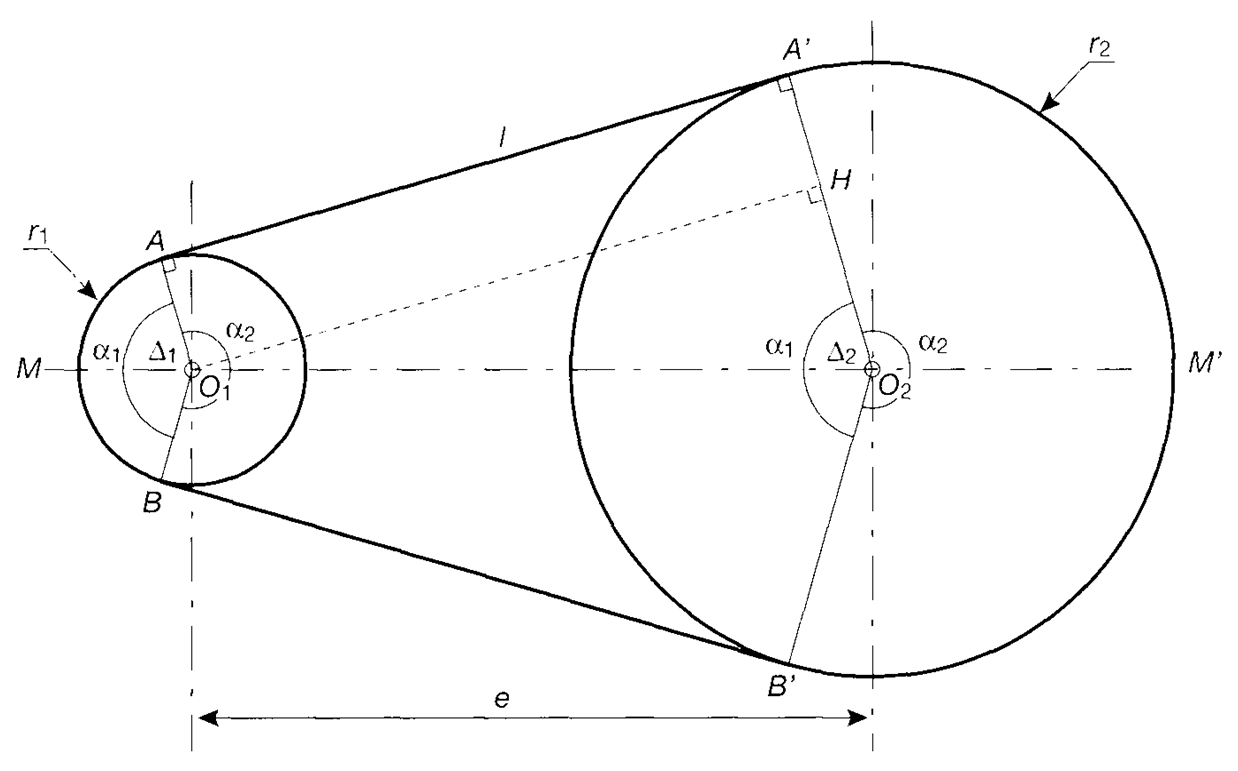
\includegraphics[width=.9\textwidth]{png/fig_43}
\end{center}
\end{minipage} \hfill
\begin{minipage}[c]{.4\linewidth}
La longueur de courroie est dans ce cas donnée par : 
$$
L = 2e\sin\dfrac{\alpha_1}{2}+r_1 \alpha_1 + r_2 \left( 2\pi - \alpha_1\right)
$$
  
avec $\cos \dfrac{\alpha_1}{2} = \dfrac{r_2-r_1}{e}$.


\end{minipage} 


\subsubsection{Tension dans les brins de la courroie}

\begin{minipage}[c]{.55\linewidth}
\begin{center}
\includegraphics[width=.9\textwidth]{png/fig_44}
\end{center}
\end{minipage} \hfill
\begin{minipage}[c]{.4\linewidth}
En isolant la poulie réceptrice 2, on voit qu’elle est soumise, à l’équilibre, à l’action du brin tendu $\vect{T}$, du brin mou $\vect{t}$, d’un couple résistant $\vect{C_2}$ et de l’action du bâti en $O_2$.

Le théorème du moment statique exprimé en $O_2$, nous donne en projection sur $\vect{z}$:
$$
T - t = \dfrac{C_2}{r_2}= \dfrac{C_1}{r_1}
$$
\end{minipage} 


La détermination du couple se fait connaissant la puissance à transmettre ainsi que la vitesse de rotation :
$C_1 = \dfrac{\mathcal{P}}{\omega_1}$ et  $C_2 = \dfrac{\mathcal{P}}{\omega_2}$  (cas où le rendement est unitaire $\eta = 1$).

Il faut une 2nd relation pour connaître individuellement $T$ et $t$.

Prenons le cas d’une courroie plate.

On néglige les effets dynamiques, ainsi que l’action de la pesanteur.

On démontre alors qu’à la limite du glissement :  $T=t\cdot e^{f\alpha}$.


En pratique, pour l’application de cette formule, on choisit l’angle d’enroulement de la plus petite poulie, car c’est sur elle, qu’apparaît en premier le glissement.

Dans le cas d’une courroie trapézoïdale, on obtient  $T=t\cdot e^{\dfrac{f\alpha}{\sin \delta}}$.

\begin{minipage}[c]{.25\linewidth}
\begin{center}
\includegraphics[height=3cm]{png/fig_45}
\end{center}
\end{minipage} \hfill
\begin{minipage}[c]{.7\linewidth}
Souvent, $\delta=20^o$. On a alors $T\simeq t\cdot e^{3f\alpha}$.
L’intérêt d’une courroie trapézoïdale par rapport à une courroie plate est que le couple transmissible est plus important à tension de pose identique, et que les efforts radiaux sur l’arbre sont moindres à couple transmis identique.

\end{minipage} 

\subsubsection{Tension de pose}
Pour avoir les tensions $\vect{T}$ et $\vect{t}$ en fonctionnement, il faut appliquer une tension initiale à l’arrêt, appelée tension de pose $T_0$, sur les brins de la courroie.

On montre alors que  $T+t=2T_0$.

\begin{minipage}[c]{.45\linewidth}
\begin{center}
\includegraphics[width=.9\textwidth]{png/fig_46}
\end{center}
\end{minipage} \hfill
\begin{minipage}[c]{.5\linewidth}
La valeur de la tension de pose est souvent contrôlée par la mesure de la flèche du brin rectiligne, sous un effort normal F, appliqué en son milieu.
\end{minipage} 

L’usure et le vieillissement de la courroie entraînent une diminution progressive de la tension de pose.

\subsubsection{Différents types de courroie}

\begin{center}
\includegraphics[height=5cm]{png/fig_47}
\end{center}


\begin{minipage}[c]{.6\linewidth}
La transmission de puissance par courroie synchrone (ou crantée), associée à des poulies dentées, permet d’éviter le glissement. On les utilise par exemple pour les courroies de distribution d’automobiles ou pour les systèmes asservis en position où un positionnement précis est nécessaire.

L’entraînement ne se fait plus par adhérence, mais par obstacle, comme dans le cas des engrenages.

Le dimensionnement de la transmission est essentiellement basé sur la capacité de la courroie à supporter l’effort de traction.

\end{minipage} \hfill
\begin{minipage}[c]{.35\linewidth}
\begin{center}
\includegraphics[height=3cm]{png/fig_48}
\end{center}
\end{minipage} 

\subsection{La transmission de puissance par chaîne}

Une chaîne est un lien déformable destiné à assurer une transmission de puissance entre un arbre moteur et un arbre récepteur, dont les axes sont parallèles. Il n’y a pas d’inversion de sens de rotation.



\begin{minipage}[c]{.55\linewidth}
La plupart du temps, la chaîne travaille en traction, sauf certaines chaînes spécifiques qui peuvent être « poussées ».
La transmission par chaîne présente les avantages suivants :
\begin{itemize}
\item puissances transmises importantes ;
\item possibilité de variation d’entraxe ;
\item pas de glissement ;
\item aptitude à fonctionner dans des conditions sévères (choc, température, etc.) ;
\item efforts limités sur les paliers ;
\item rendement (98 \%) ;
\item coût réduit.
\end{itemize}
\end{minipage} \hfill
\begin{minipage}[c]{.4\linewidth}
\begin{center}
\includegraphics[height=4cm]{png/fig_49}
\end{center}
\end{minipage}

Les inconvénients de ce type de transmission sont principalement :
\begin{itemize}
\item nécessité d’une lubrification ;
\item niveau sonore important ;
\item vibrations longitudinales ;
\item limitation du rapport de transmission.
\end{itemize}
L’entraînement se fait par obstacle. Le dimensionnement de la transmission est essentiellement basé sur la capacité de la chaîne à supporter l’effort de traction. De même que pour les courroies, on peut utiliser un dispositif assurant la tension constante de la chaîne.

\subsubsection{Comportement cinématique}
 La transmission devient quasiment homocinétique à partir d’un nombre de dents, sur le plus petit pignon, de 20.

\begin{minipage}[c]{.45\linewidth}
\begin{center}
\includegraphics[width=.9\textwidth]{png/fig_50}
\end{center}
\end{minipage} \hfill
\begin{minipage}[c]{.5\linewidth}
Le rapport de transmission moyen est donné par,  $\dfrac{\omega_2}{\omega_1}=\dfrac{r_1}{r_2}$.
Au cas où le nombre de dents est important $\pi \cdot d_p \simeq p\cdot Z_d$.
Le rapport de transmission peut alors être donné par $\dfrac{\omega_2}{\omega_1}=\dfrac{Z_1}{Z_2}$.

\end{minipage} 

\subsubsection{Longueur de chaîne}
\paragraph{Longueur théorique}
\begin{center}
\includegraphics[height=4cm]{png/fig_51}
\end{center}

Soit $L$ la longueur de la chaîne et $e$ l'entraxe.


On montre que :  
$$L=2e\cos\alpha + \dfrac{p}{2} \left( \dfrac{\pi - 2\alpha}{\sin \dfrac{\pi }{Z_1}} + \dfrac{\pi + 2\alpha}{\sin \dfrac{\pi }{Z_2}}\right)$$


avec $\alpha$ donné par $\sin \alpha = \dfrac{r_2-r_1}{e}$.


Il est habituel d’exprimer une longueur de chaîne en nombre de maillons : $L_m = \dfrac{L}{p}$.
$$
L_m \simeq \dfrac{2e \cos \alpha}{p} +\dfrac{Z_1+Z_2}{2} +\dfrac{\alpha \left( Z_2-Z_1\right)}{\pi}
$$

\paragraph{Longueur réelle}
La longueur réelle de la chaîne dépend du pas p et du nombre entier de maillons qui la compose.
Pour ce genre de chaîne, le nombre de maillons est forcément pair :

\begin{minipage}[c]{.45\linewidth}
\begin{center}
\includegraphics[height=3cm]{png/fig_52}
\end{center}
\end{minipage} \hfill
\begin{minipage}[c]{.45\linewidth}
\begin{center}
\includegraphics[height=3cm]{png/fig_53}
\end{center}
\end{minipage} 

D’autres chaînes, peuvent avoir un nombre pair ou impair de maillons :
\begin{minipage}[c]{.45\linewidth}
\begin{center}
\includegraphics[height=2.5cm]{png/fig_54}
\end{center}
\end{minipage} \hfill
\begin{minipage}[c]{.45\linewidth}
\begin{center}
\includegraphics[height=3cm]{png/fig_55}
\end{center}
\end{minipage} 

\subsubsection{Représentation schématique}

\begin{center}
\includegraphics[width=.75\textwidth]{png/fig_56}
\end{center}


\subsection{La transmission de puissance par engrenage}
Les engrenages ont pour fonction de transmettre la puissance, les deux vitesses (entrée et sortie) restant dans un rapport constant, c’est une transmission homocinétique.
Les solutions concurrentes :
\begin{itemize}
\item transmission par accouplement, les arbres devant être dans le prolongement l’un de l’autre;
\item transmission par friction : roues de friction, courroies plates ou courroies trapézoïdales sur poulies;
\item transmission par courroie crantée sur poulies ou par chaîne sur roues.
\end{itemize}
Pour un prix de revient modéré, les engrenages ont pour avantages un excellent rendement et un encombrement plutôt faible.

\begin{minipage}[c]{.5\linewidth}
Un engrenage est un ensemble de deux roues dentées complémentaires, chacune en liaison (pivot ou glissière) par rapport à un support (souvent le bâti).
La petite roue se nomme le pignon, la grande roue extérieure s’appelle la roue, la grande roue intérieure s’appelle la couronne. L’une des roues peut avoir un rayon infini, elle s’appelle alors une crémaillère.

\end{minipage} \hfill
\begin{minipage}[c]{.45\linewidth}
\begin{center}
\includegraphics[width=.8\textwidth]{png/fig_57}
\end{center}
\end{minipage} 

Le rapport de transmission $k$ est par définition :  $k = \dfrac{\omega_{entree}}{\omega_{sortie}}$.

On appelle surfaces primitives, les surfaces fictives des roues de friction associées donnant la même cinématique que l’engrenage. Les profils de denture sont en général des développantes de cercle.

\subsubsection{Propriétés géométriques de la développante de cercle}

Une développante de cercle est caractérisée par le rayon du cercle de base. Toutes les développantes d’un même cercle sont des courbes parallèles. Pour un fonctionnement sans frottement, l’action de la roue 1 sur la roue 2 est un glisseur de module fixe, d’axe central fixe $(I,\vect{u})$ , si le couple transmis est constant. 



\begin{minipage}[c]{.4\linewidth}
\begin{center}
\includegraphics[width=.9\textwidth]{png/fig_58}
\end{center}

\end{minipage} \hfill
\begin{minipage}[c]{.55\linewidth}
Soient $r_1$ et $r_2$ les rayons primitifs; $Z_1$ et $Z_2$ les nombres de dents; $a$ l’entraxe.
On démontre alors que : $\dfrac{2\pi r_1}{Z_1}=\dfrac{2\pi r_2}{Z_2}=\dfrac{2\pi a}{Z_1+Z_2}=p$.

Le paramètre « p » est une caractéristique du fonctionnement de l’engrenage, il est appelé pas de fonctionnement ; nous pouvons alors définir le module « m » de fonctionnement :

$r_1=\dfrac{mZ_1}{2}$, $r_1=\dfrac{mZ_2}{2}$, $r_1=\dfrac{mZ_1}{2}$
Le module $m$ s’exprime en $mm$ et il possède des valeurs normalisées $(… ; 0,5 ; 0,75 ; 1 ; …)$.

\end{minipage}

\subsubsection{Propriétés cinématiques}
Le module de la vitesse de glissement entre la roue 1 et la roue 2 au point de contact $M$ augmente lorsque le point $M$ s’éloigne du point de tangence des cercles primitifs, I :
$\vectv{M}{2}{1}=\lambda\left(\omega(2/0)-\omega(1/0) \right)\vect{v}$ avec $\vect{IM} = \lambda \vect{u}$

De plus, cette vitesse de glissement change de signe lorsque $M$ passe par $I$. Ainsi en prenant en compte le frottement au contact des dentures, la composante tangentielle (portée par $\vect{v}$) de l’action de la roue 1 sur la roue 2, change de signe au point $I$. Ceci peut être générateur de vibrations et entraîner la rupture du film d’huile. Pour améliorer la durée de vie de l’engrenage, il est nécessaire d’utiliser une lubrification adaptée et de limiter cette vitesse de glissement.

\subsubsection{Fabrication des engrenages}
Par moulage : au sable, pour solides en fonte ou en acier, sous pression pour roues en alliages légers, ou matières plastiques. Les dentures sont très souvent achevées sur une machine à tailler.

Par forgeage : il donne également des dentures brutes.

Par taillage :	
\begin{itemize}
\item taillage successif : les dents sont usinées complètement et successivement par une fraise de forme;
\item taillage progressif : à chaque instant toutes les dents à tailler sont à peu près dans le même état avec la génération par vis mère ou par outil crémaillère, ou encore par outil- pignon.
\end{itemize}

\begin{minipage}[c]{.45\linewidth}
\begin{center}
\includegraphics[height=3cm]{png/fig_59}
\end{center}
\end{minipage} \hfill
\begin{minipage}[c]{.45\linewidth}
\begin{center}
\includegraphics[height=3cm]{png/fig_60}
\end{center}
\end{minipage}

\begin{minipage}[c]{.45\linewidth}
\begin{center}
\includegraphics[height=3cm]{png/fig_61}
\end{center}
\end{minipage} \hfill
\begin{minipage}[c]{.45\linewidth}
\begin{center}
\includegraphics[height=3cm]{png/fig_62}
\end{center}
\end{minipage}


\subsubsection{Les engrenages cylindriques à denture droite}

\begin{minipage}[c]{.3\linewidth}
\begin{center}
\includegraphics[height=3cm]{png/fig_63}
\end{center}
\end{minipage} \hfill
\begin{minipage}[c]{.3\linewidth}
\begin{center}
\includegraphics[height=3cm]{png/fig_64}
\end{center}
\end{minipage}\hfill
\begin{minipage}[c]{.3\linewidth}
\begin{center}
\includegraphics[height=3cm]{png/fig_65}
\end{center}
\end{minipage}

Les roues extérieures tournent en sens contraires alors que pour un engrenage intérieur, les deux roues tournent dans le même sens.

Relations géométriques $d=m\times Z $ et $a=\dfrac{d_1+d_2}{2}$.

Efforts sur la denture :

\begin{center}
\includegraphics[width=.7\textwidth]{png/fig_66}
\end{center}

Soit $\mathcal{P}_1$ la puissance à transmettre. On a la relation pour un solide en rotation autour d’un axe fixe : $\mathcal{P}_1=C_1 \omega_1$, qui lie la puissance (en Watt) au couple (en $N.m$) et à la vitesse de rotation (en $rad/s$).

Si le rendement de la transmission est $\eta=1$, $\mathcal{P}_2 = C_2 \omega_2 = C_1 \omega_1$.

On peut donc déterminer le couple $C_1$, connaissant la puissance et la vitesse de rotation.

L’effort tangentiel s’obtient à l’aide du couple, sachant que  $F_T = \dfrac{C_1}{r_1}$.

On peut ensuite en déduire la composante radiale $F_R$ et la norme de l’effort mutuel qu’exerce une roue sur l’autre, connaissant l’angle de pression $\alpha$ (valeur usuelle 20 degrés).

Notons que dans le cas où la transmission n’est pas idéale, $\eta\neq 1$ .


\subsubsection{Les engrenages cylindriques à denture hélicoïdale}
Les engrenages à denture hélicoïdale permettent un fonctionnement plus silencieux que celui des engrenages à denture droite ; ils présentent également un meilleur rendement. Ils sont notamment utilisés dans les boîtes de vitesses d’automobiles, les réducteurs et les multiplicateurs de vitesses.

\begin{center}
\includegraphics[height=3cm]{png/fig_67}
\includegraphics[height=3cm]{png/fig_68}
\end{center}

\begin{itemize}
\item Hélice primitive : intersection d’un flanc avec le cylindre primitif d’une roue hélicoïdale;
\item angle d’hélice $\beta$ : angle entre la tangente à l’hélice primitive et une génératrice du cylindre primitif;
\item pas apparent $p_t$ : longueur de l’arc de cercle primitif compris entre deux profils homologues consécutifs;
\item pas réel $p_n$ : pas mesuré sur une hélice normale à l’hélice primitive;
\item module apparent $m_t$ : rapport entre le pas apparent et le nombre de dents;
\item module réel $m_n$ : rapport entre le pas réel et le nombre de dents.
\end{itemize}


\begin{minipage}[c]{.65\linewidth}
Quel que soit le diamètre, les roues dentées à denture hélicoïdale de même module et de même angle d’hélice engrènent entre elles, à condition que les hélices soient de sens contraire.
Les dentures hélicoïdales provoquent une poussée axiale, proportionnelle à l’angle d’hélice $\beta$. On peut donc réduire la poussée axiale en diminuant l’angle d’hélice, mais on peut également la supprimer, en utilisant des roues jumelées dont les dentures sont inclinées en sens opposé ou encore par l’utilisation d’une denture en chevrons.
\end{minipage} \hfill
\begin{minipage}[c]{.3\linewidth}
\begin{center}
\includegraphics[height=5cm]{png/fig_69}
\end{center}
\end{minipage}

Relations géométriques : $d=m_t Z$ et $a=\dfrac{d_1+d_2}{2}$.

Efforts sur les dentures : 
\begin{center}
\includegraphics[width=.75\textwidth]{png/fig_70}
\end{center}

L’angle de pression réel est noté $\alpha_n$.

De même que pour une denture droite, à partir de la puissance à transmettre, on détermine l’effort tangentiel, puis les autres composantes.

\subsubsection{Les engrenages coniques}
Les engrenages coniques sont des engrenages à axes concourants. Ils permettent de transmettre le mouvement entre deux arbres concourants, avec un rapport de vitesse rigoureux. Les conditions d’engrènement imposent que les deux roues doivent avoir même module et que les sommets des deux cônes soient confondus. Ce dernier impératif oblige le concepteur à un centrage très précis des deux roues pour assurer un fonctionnement correct. Il faut donc prévoir au montage un réglage axial des deux roues. On peut utiliser par exemple des boîtiers et des cales de réglage.

Cône primitif, angle primitif $\delta$ : cône décrit par l’axe instantané de rotation du mouvement relatif de la roue conjuguée par rapport à la roue considérée. Le demi angle au sommet de ce cône est l’angle primitif $\delta$.
Diamètre primitif $d$ : diamètre du cercle intersection du cône primitif et du cône complémentaire (cercle primitif).

\begin{center}
\includegraphics[height=3cm]{png/fig_71}
\end{center}

Relations géométriques : $\tan \delta_1 = \dfrac{Z_1}{Z_2}$ : $d_1 = m\cdot Z_1$ et $d_2 = m\cdot Z_2$.

Efforts sur les dentures : 

\begin{minipage}[c]{.5\linewidth}
\begin{center}
\includegraphics[width=.45\textwidth]{png/fig_72}
\includegraphics[width=.45\textwidth]{png/fig_73}
\end{center}
\end{minipage} \hfill
\begin{minipage}[c]{.45\linewidth}
\begin{itemize}
\item $F_A = F_T \tan \alpha_n \sin \delta$
\item $F_R = F_T \tan \alpha_n \cos \delta$
\item $F = \dfrac{F_T}{\cos \alpha_n}$
\item $F = \sqrt{F_T^2+F_A^2+F_R^2}$
\end{itemize}
L'angle de pression est noté $\alpha_n$. 
A partir de la puissance à transmettre, on déterminer l'effort tangentiel à l'aide du rayon moyen $r_m$ : $r_m = \dfrac{d-b\sin\delta}{2}$. On déterminer alors les autres composantes. 
\end{minipage}

\subsubsection{Cas d'un engrenage gauche : le système roue et vis sans fin}
\begin{minipage}[c]{.65\linewidth}
C’est un engrenage hélicoïdal dont les axes sont orthogonaux et non concourants.
La transmission par ce type d’engrenage donne une solution simple pour les grands rapports de réduction, avec un fonctionnement peu bruyant. La poussée de la vis est forte, surtout si la démultiplication est grande. On utilise alors une butée à billes ou à rouleaux ou encore des roulements à contact oblique pour réaliser la liaison pivot avec le support. Lorsque l’inclinaison des filets est faible (vis à un filet et inclinaison inférieure à 5 degrés), la transmission est irréversible, ce qui est souvent utile, car le réducteur s’oppose à toute rotation commandée par la machine réceptrice (exemple : appareils de levage).
Toutefois le rendement est alors faible, et de plus le couple de démarrage est beaucoup plus fort que le couple à vitesse de régime. Le rendement est meilleur avec les fortes inclinaisons, à condition que les métaux en présence soient bien choisis (vis en acier / roue en bronze, nylon, …) et l’exécution des dentures très précises, avec des états de surface très soignés.
\begin{center}
\end{center}
\end{minipage} \hfill
\begin{minipage}[c]{.3\linewidth}
\includegraphics[width=.8\textwidth]{png/fig_74}
\includegraphics[width=.8\textwidth]{png/fig_75}
\end{minipage}

Pour la vis :
\begin{itemize}
\item Filet : une des dents de la vis. Les vis peuvent avoir un ou plusieurs filets.
\item Cylindre de référence : surface primitive de référence de la vis.
\item Hélice de référence : hélice d’intersection d’un flanc avec le cylindre de référence de la vis.
\item Pas hélicoïdal $p_z$ : distance axiale entre deux profils homologues consécutifs d’un filet.
\item Pas axial $p_x$ : rapport entre le pas hélicoïdal et le nombre de filets (le pas axial est égal au pas hélicoïdal si le nombre de filets est égal à 1).
\item Module axial $m_x$: rapport entre le pas et le nombre $\pi$.
\end{itemize}

Pour la roue : 
Le profil de la roue est le profil conjugué de celui de la vis. L’engrènement d’une vis avec une roue n’est possible que si elles ont même module axial et même angle d’hélice. Les caractéristiques dimensionnelles de la roue sont identiques à celles d’une roue à denture hélicoïdale. La roue est généralement cylindrique pour transmettre des efforts relativement faibles, mais pour transmettre des efforts importants, une roue creuse est préférable.

\begin{center}
\includegraphics[width=.75\textwidth]{png/fig_76}
\end{center}


\begin{minipage}[c]{.45\linewidth}
\begin{center}
\includegraphics[width=.8\textwidth]{png/fig_77}
\end{center}
\end{minipage} \hfill
\begin{minipage}[c]{.45\linewidth}
\begin{center}
\includegraphics[width=.8\textwidth]{png/fig_78}
\end{center}
\end{minipage} \hfill


\begin{minipage}[c]{.45\linewidth}
\begin{center}
\includegraphics[width=.9\textwidth]{png/fig_79}
\end{center}
\end{minipage} \hfill
\begin{minipage}[c]{.45\linewidth}
Si le frottement est négligé : $\eta=1$ :
\begin{itemize}
\item $F_{Tv}=F_{Ar} = \dfrac{C_v}{r_v}$;
\item $F_{Av}=F_{Tr} = \dfrac{F_{Tv}}{\tan \beta}$;
\item $F_R = F_{Tv} \dfrac{\tan \alpha_n }{\sin \beta}$;
\item $F = \dfrac{F_R}{\sin \alpha_n}$.
\end{itemize}

Rendement :
$$
\eta = \dfrac{\cos \alpha_n - f\tan \beta}{\cos \alpha_n + f\cos \beta}
$$

\end{minipage} 

\subsection{Les trains d'engrenages}
Le train d’engrenage est la façon la plus répandue de réaliser des réducteurs ou des multiplicateurs.
\subsubsection{Les trains d'engrenages simples}

On appelle train d’engrenages simple (ou ordinaire), un train pour lequel tous les roues dentées tourne autour d’un axe fixe par rapport au carter.

\paragraph{Les réducteurs élémentaires}
\begin{center}
\includegraphics[width=.8\textwidth]{png/fig_80}
\end{center}
\begin{center}
\includegraphics[width=.8\textwidth]{png/fig_81}

\textit{Exemple : réducteur roue et vis sans fin}
\end{center}

\subsubsection{Les trains d'engrenages simples}
Loi entrée -- sortie : $\dfrac{\omega_{s/0}}{\omega_{e/0}}=r$, $r=(-1)^p \dfrac{\text{Produit du nombre de dents des menantes}}{\text{Produit du nombre de dents menées}}$
\begin{itemize}
\item $p$ : nombre de contacts extérieurs;
\item $\omega{s/0}$ : vitesse de rotation de la dernière roue;
\item $\omega{e/0}$ : vitesse de rotation de la première roue.
\end{itemize}

Lorsque cela est possible, on peut remplacer des rapports de nombre de dents par des rapports de diamètres primitifs.

Exemples : 

\begin{center}
\includegraphics[width=.8\textwidth]{png/fig_82}
\end{center}


\begin{center}
\includegraphics[width=.8\textwidth]{png/fig_83}

\textit{Réducteur à deux étages à axes orthogonaux}
\end{center}


\subsubsection{Les trains épicycloïdaux}

Un train d'engrenages est qualifié d'épicycloïdal quand, pendant le fonctionnement, une ou plusieurs roues dentées tournent autour d'un axe géométrique mobile par rapport au carter principal.


\begin{minipage}[c]{.55\linewidth}
La formule de Willis permet de déterminer la loi entrée -- sortie dans les trains épicycloïdaux :
$$
r = \dfrac{\omega(s/0)-\omega(ps/0)}{\omega(e/0)-\omega(ps/0)}
$$
avec : 
\begin{itemize}
\item $r$: raison de base : 
$$r=(-1)^p \dfrac{\text{Produit du nombre de dents des menantes}}{\text{Produit du nombre de dents menées}}$$;
\item $p$ : nombre de contacts extérieurs ;
\item $\omega(s/0)$  : vitesse de rotation de la dernière roue ;
\item $\omega(ps/0)$  : vitesse de rotation du bras porte-satellite ;
\item $\omega(e/0)$  : vitesse de rotation de la première roue.
\end{itemize} 
\end{minipage} \hfill
\begin{minipage}[c]{.4\linewidth}
\begin{center}
\includegraphics[width=.8\textwidth]{png/fig_84}
\end{center}
\end{minipage} 

Différentes configurations sont possibles :


\begin{center}
\includegraphics[width=.8\textwidth]{png/fig_85}
\end{center}

\begin{center}
\includegraphics[width=.8\textwidth]{png/fig_86}
\end{center}

\begin{center}
\includegraphics[width=.8\textwidth]{png/fig_87}

\textit{Exemple : Moteur à palettes}
\end{center}


\subsubsection{Les boîtes de vitesse}

Lorsque l’organe récepteur oppose un couple résistant d’intensité variable, il peut être nécessaire d’utiliser une boîte de vitesse. Le rapport de fréquences de rotation entre l’arbre d’entrée (sortie moteur thermique) et l’arbre de sortie (entrée différentiel) est variable.

Pour des boîtes de vitesse étagées, il existe plusieurs rapports de transmission, selon la sélection.

Exemple : véhicule automobile avec 4 rapports + marche arrière
$K_1=-0,24$ ; $K_2=-0,54$ ; $K_3=-0,86$ ; $K_4=-1,21$ ;$K_{AR}=0,3$.

Le passage des vitesses peut se faire manuellement (levier de vitesse) ou automatiquement.
La commande au niveau de la boîte peut être mécanique, hydraulique ou électro-hydraulique.


\begin{minipage}[c]{.2\linewidth}
\begin{center}
\includegraphics[height=3cm]{png/fig_88}

\textit{Fourchette}
\end{center}
\end{minipage} \hfill
\begin{minipage}[c]{.2\linewidth}
\begin{center}
\includegraphics[height=3cm]{png/fig_89}

\textit{Crabot}
\end{center}
\end{minipage} \hfill
\begin{minipage}[c]{.2\linewidth}
\begin{center}
\includegraphics[height=3cm]{png/fig_90}

\textit{Synchroniseur}
\end{center}
\end{minipage} \hfill
\begin{minipage}[c]{.2\linewidth}
\begin{center}
\includegraphics[height=3cm]{png/fig_91}
\end{center}
\end{minipage} 


\begin{minipage}[c]{.4\linewidth}
\begin{center}
\includegraphics[width=.8\textwidth]{png/fig_92}

\textit{Boîte de vitesse à commande mécanique manuelle  Renault}
\end{center}
\end{minipage} \hfill
\begin{minipage}[c]{.55\linewidth}
\begin{center}
\includegraphics[width=.8\textwidth]{png/fig_93}

\textit{Boîte de vitesse robotisée Renault}

\end{center}
\end{minipage}


Certaines boîtes de vitesse sont à variation continue (CVT).


\begin{center}
\includegraphics[width=.7\textwidth]{png/fig_94}

\textit{Boîte de vitesse à variation continue Audi}

\end{center}


\section{La transmission de l’énergie avec transformation de mouvement}

\subsection{La transmission de puissance par mécanisme Vis -- Ecrou}

\subsubsection{Fonctions techniques d’une liaison hélicoïdale}

Les fonctions techniques de la liaison hélicoïdale sont :
\begin{itemize}
\item transformer un mouvement.
\end{itemize}
Les paramètres importants sont notamment le jeu dans la liaison et la vitesse de glissement au contact vis / écrou.
\begin{itemize}
\item transmettre un effort.
\end{itemize}

Les déformations, le frottement, les pressions de contact sont des paramètres importants.

On distingue principalement deux types de réalisation de liaison hélicoïdale :
\begin{itemize}
\item à contact glissant;
\item à éléments roulants.
\end{itemize}


\begin{minipage}[c]{.45\linewidth}
\begin{center}
\includegraphics[height=3cm]{png/fig_95}
%\textit{Boîte de vitesse à commande mécanique manuelle  Renault}
\end{center}
\end{minipage} \hfill
\begin{minipage}[c]{.45\linewidth}
\begin{center}
\includegraphics[height=3cm]{png/fig_96}
\end{center}
\end{minipage}



\begin{minipage}[c]{.45\linewidth}
\begin{center}
\includegraphics[height=3cm]{png/fig_97}

\includegraphics[height=3cm]{png/fig_98}
\end{center}
\end{minipage} \hfill
\begin{minipage}[c]{.45\linewidth}
\begin{center}
\includegraphics[height=3cm]{png/fig_99}

\includegraphics[height=3cm]{png/fig_100}
\end{center}
\end{minipage}

\subsubsection{Les montages courants}

\begin{center}
\includegraphics[width=.8\textwidth]{png/fig_101}
\end{center}

On définit le rendement du transmetteur en régime permanent par :
$$
\eta = \dfrac{|F(c\rightarrow 2) \times V_{2/0}|}{C(m\rightarrow 1)\times \omega_{1/0}}=\left| \dfrac{F(c\rightarrow 2)}{C(m\rightarrow 1)}\right|\times \dfrac{p}{2\pi}
$$

Si les pertes par frottements sont négligées, alors $\eta=1$ et :
\begin{itemize}
\item cas d'une hélice à droite : $C(m\rightarrow 1) = \dfrac{F(c\rightarrow 2)\times p}{2\pi}$;
\item cas d'une hélice à gauche : $C(m\rightarrow 1) = -\dfrac{F(c\rightarrow 2)\times p}{2\pi}$.
\end{itemize}

Pour un effort résistant donné, il vaut mieux choisir un pas p petit pour limiter le couple moteur, mais la vitesse de translation est alors faible.

Le nombre de filets n’intervient pas dans la loi entrée / sortie cinématique, c’est uniquement le pas $p$ qui est à prendre en compte.

On appelle pas réduit le paramètre $\lambda = \dfrac{p}{2\pi}$ ($m/rad$).


\begin{center}
\includegraphics[width=.8\textwidth]{png/fig_102}
\end{center}

Afin d’améliorer le rendement, il existe des mécanismes vis / écrou avec recirculation de billes.
La réversibilité peut être obtenue pour un angle d’hélice $\alpha$ supérieur à $\varphi$ avec :
\begin{itemize}
\item $\tan\alpha=\dfrac{p}{2\pi R}$ ($R$ : rayon moyen de la vis);
\item $f=\tan \varphi$ ($f$ : facteur de frottement au contact vis/écrou).
\end{itemize}

\begin{center}
\includegraphics[width=.8\textwidth]{png/fig_103}
\end{center}

Le guidage en rotation de la vis peut nécessiter un nombre plus ou moins important de paliers :
\begin{center}
\includegraphics[width=.4\textwidth]{png/fig_104}
\end{center}

En fonction de la rigidité du montage souhaité et de la puissance dissipée, la liaison glissière peut être réalisée de diverses manières :

\begin{minipage}[c]{.3\linewidth}
\begin{center}
\includegraphics[height=3cm]{png/fig_105}
\end{center}
\end{minipage} \hfill
\begin{minipage}[c]{.3\linewidth}
\begin{center}
\includegraphics[height=3cm]{png/fig_106}
\end{center}
\end{minipage}\hfill
\begin{minipage}[c]{.3\linewidth}
\begin{center}
\includegraphics[height=3cm]{png/fig_107}
\end{center}
\end{minipage}

\begin{minipage}[c]{.2\linewidth}
\begin{center}
\includegraphics[height=3cm]{png/fig_108}
\end{center}
\end{minipage}\hfill
\begin{minipage}[c]{.75\linewidth}
\begin{center}
\includegraphics[width=\textwidth]{png/fig_109}
\end{center}
\end{minipage}

Afin de diminuer ou d’éliminer l’hyperstatisme du montage classique, il est possible de réaliser un aménagement par écrou flottant :

\begin{center}
\includegraphics[width=.8\textwidth]{png/fig_110}
\end{center}

\begin{center}
\includegraphics[width=\textwidth]{png/fig_111}
\end{center}

\begin{center}
\includegraphics[width=.8\textwidth]{png/fig_112}
\end{center}

\subsection{La transmission de puissance par mécanismes articulés}
Après avoir sélectionné un actionneur, il peut être nécessaire de modifier la nature du mouvement.
Ce qui suit, présente quelques principes de transformation de mouvement, à l’aide de mécanismes plans.

\subsubsection{Le système bielle / manivelle}

Le système bielle / manivelle (ou vilebrequin) permet de transformer une rotation continue en une translation rectiligne alternative. On le retrouve dans la réalisation des moteurs thermiques, compresseurs, etc.


\begin{minipage}[c]{.45\linewidth}
\begin{center}
\includegraphics[width=.9\textwidth]{png/fig_113}
\end{center}
\end{minipage}\hfill
\begin{minipage}[c]{.5\linewidth}
\begin{center}
\includegraphics[width=.9\textwidth]{png/fig_114}
\end{center}
\end{minipage}

\subsubsection{Les systèmes à excentriques}

\begin{center}
\includegraphics[width=.8\textwidth]{png/fig_115}

\textit{Pompe à pistons radiaux}
\end{center}

\subsubsection{Les systèmes à cames}

Les systèmes à came, transforment un mouvement de rotation en un mouvement de translation rectiligne alternative. L’exemple ci-dessous montre un moteur de Porsche (V8) dans lequel, on peut voir le système bielle manivelle et le mécanisme arbre à came / soupape. 

\begin{center}
\includegraphics[width=.95\textwidth]{png/fig_117}
\end{center}

\begin{minipage}[c]{.3\linewidth}
\begin{center}
\includegraphics[height=4cm]{png/fig_118}
\end{center}
\end{minipage}\hfill
\begin{minipage}[c]{.3\linewidth}
\begin{center}
\includegraphics[height=4cm]{png/fig_119}
\end{center}
\end{minipage}\hfill
\begin{minipage}[c]{.3\linewidth}
\begin{center}
\includegraphics[height=4cm]{png/fig_120}
\end{center}
\end{minipage}


\begin{center}
\includegraphics[width=.8\textwidth]{png/fig_121}

\textit{Indexeur à came}
\end{center}


\subsubsection{Système à excentriques à biellette}
Le variateur GUSA étudié permet d’obtenir une rotation intermittente de l’arbre de sortie 8 à partir d’une rotation continue de l’arbre d’entrée 1.
L’ensemble 2+3+4 permet d’obtenir une rotation alternée de 7.
L’amplitude de cette oscillation se règle avec le volant 12 qui permet de translater la pièce 5.
Une roue libre placée entre 7 et 8 permet de n’entraîner l’arbre de sortie que dans un sens (encliquetage indiqué sur le dessin).
L’arbre de sortie peut ainsi, sur une chaîne automatisée, engendrer l’avance pas à pas, réglable d’un tapis.

\begin{minipage}[c]{.47\linewidth}
\begin{center}
\includegraphics[width=.95\textwidth]{png/fig_122}
\end{center}
\end{minipage}\hfill
\begin{minipage}[c]{.47\linewidth}
\begin{center}
\includegraphics[width=.95\textwidth]{png/fig_123}
\end{center}
\end{minipage}


\subsubsection{Mécanisme à croix de Malte}
\begin{minipage}[c]{.45\linewidth}
\begin{center}
\includegraphics[width=.8\textwidth]{png/fig_124}
\end{center}
\end{minipage}\hfill
\begin{minipage}[c]{.45\linewidth}
Le mécanisme à croix de malte assure la transformation d'un mouvement de rotation continu en un mouvement de rotation intermittent, appelé couramment pas à pas.
Ce mécanisme comprend un arbre moteur animé d'un mouvement de rotation continu uniforme, muni de un ou plusieurs manetons, et un plateau mené, muni de rainures, le plus souvent rectilignes. Ce plateau est en liaison encastrement avec l'arbre récepteur. Un cycle de fonctionnement comprend, par tour de l'arbre moteur, une ou plusieurs périodes de mouvement, une ou plusieurs périodes d'arrêt.

\end{minipage}
\subsubsection{Le pantographe}

La potence d'équilibrage proposée est utilisée pour diminuer le roulis sur les bateaux. Les potences sont placées perpendiculairement au plan de symétrie du bateau, la charge (7) face à la mer. Si l'on écarte les charges (7), le moment d'inertie du navire par rapport à l'axe de rotation du roulis augmente, diminuant ainsi la vitesse de rotation ou roulis.
La potence se compose d'un vérin d'équilibrage à ressort (5 + 6), libre de translater horizontalement dans la rainure R, et d'un ensemble de barres articulées entre elles en pantographe avec un contrepoids (8). Les liaisons en $A$, $B$, $C$, $D$, $E$, $F$, $I$, $J$, $K$ et $L$ sont des liaisons pivots.

\begin{center}
\includegraphics[width=.8\textwidth]{png/fig_125}
\end{center}

Les points $A$, $C$ et $F$, restent alignés. Le rapport $AC/AF$ est constant.
Un déplacement vertical de la tige du vérin (et donc du point $C$), entraîne un déplacement vertical amplifié de la charge 7. 


\subsubsection{Système à vérin fixe et biellette}

La figure représente un modèle cinématique en vue de dessus d’un mécanisme de direction.
Il est constitué:
\begin{itemize}
\item du pignon de direction (7), lié au volant, en liaison pivot d'axe $(A,\vect{z})$ avec le boîtier de direction (1) supposé fixe ;
\item de la crémaillère (2), associée au piston d'un vérin hydraulique dans le cas d'une direction assistée, lié au boîtier par une liaison pivot glissant d'axe $(B,\vect{x})$ ;
\item de deux biellettes de direction (3) et (4), liées à la crémaillère (2) par des rotules de centres B et B' ;
\item des deux ensembles fusées - roues (5) et (6), supposés liés au châssis (1) par deux liaisons modélisées par des pivots dont les axes sont  $(D,\vect{z})$ et  $(D',\vect{z})$ (modélisation plane). Les ensembles (5) et (6) font par ailleurs l'objet de liaisons rotules de centres C et C' avec les biellettes.
\end{itemize}

La translation de la crémaillère, est transformée en rotation des roues.

\begin{center}
\includegraphics[width=.8\textwidth]{png/fig_126}
\end{center}

\subsubsection{Système à vérin pivotant}
On donne ci-dessous un mécanisme permettant l’usinage (fraisage) de la rainure dessinée en bas, à droite.
La translation de la tige du vérin 6, est transformée en une rotation du plateau 7.

\begin{center}
\includegraphics[width=.9\textwidth]{png/fig_127}
\end{center}

%
%
\begin{thebibliography}{2}
\bibitem{pb}{Supports de cours de Patrick Beynet, Lycée Rouvière, Toulon}
\bibitem{oldham}{\url{http://www.huco.com/UserFiles/Image/HUCO278\%20Oldham\%20coupling\%20lr.jpg}}
\bibitem{bmw}{\url{http://www.lerepairedesmotards.com/img/technique/lexique/bmw/chaine-cinematique_.jpg}}
\bibitem{ogival}{\url{http://photo.velo101.fr/2011/grande/test_16112011_1.jpg}}
\bibitem{came}{\url{http://pimpmymini.fr/shop/img/p/206-312-thickbox.jpg}}


%\bibitem{tab}{\url{http://bois.fordaq.com/fordaq/srvAuctionView.html?AucTIid=17877844}}
%\bibitem{cazeneuve}{\url{http://www.cazeneuve.fr/Cazeneuvefr/produits/Photos/Grandes/Optica360g.jpg}}
%\bibitem{mazak}{\url{http://www.mazak.eu/fr/node/1087}}
%\bibitem{plaquettes}{\url{http://www.industrie-techno.com/plaquettes-de-tournage-a-large-spectre-d-utilisation.13121}}
%%\bibitem{cf}{\textit{La cotation fonctionnelle}, PTSI -- Lycée Vauban, Brest.}
%%\bibitem{gdi}{\textit{Guide du dessinateur industriel}, André Chevalier, Éditions Hachette Technique, Editions 2004.}
%%\bibitem{jpp}{Supports de cours de Jean-Pierre Pupier, Lycée Rouvière, Toulon.}
%%\bibitem{gps}{\textit{Centre d'Études et de Rénovation Pédagogique de l'Enseignement Technique}, Exploitation du concept G.P.S. et de la normalisation pour la Spécification Géométrique des Produits.}
%%\bibitem{gps2}{\textit{Le Décodage du Dessin de Définition}, Guy Percebois, Lycée Louis Vincent -- Metz . \url{http://www.ac-nancy-metz.fr/enseign/sti/genimeca/zip/GPS/Tol\%20g\%E9o\%20pr\%E9\%20bac.pdf}}
%%\bibitem{rb}{Supports de cours de Renan Bonnard,PTSI, Lycée Newton, Clichy la Garenne}
%%\bibitem{jb}{Supports de cours de Joël Boiron, PTSI, Lycée Gustave Eiffel, Bordeaux}
%%\bibitem{mc}{Supports de cours de Maryline Carrez, Lycée Jules Haag, Besançon}
%%\bibitem{pf}{Supports de cours de Philippe Fichou, Lycée Vauban, Brest \url{http://philippe.fichou.pagesperso-orange.fr/documents/liaisoncomplete2003.pdf}}
%\bibitem{larousse}{\url{http://www.larousse.fr/encyclopedie/data/images/1001962-Tournage.jpg}}
%\bibitem{mandrin}{\url{http://www.machine-outil.com/gfx/produits/grand/1601-mandrin-tour-smw-autoblok.jpg}}
%\bibitem{mandrin}{\url{http://www.machine-outil.com/gfx//photos/grand/4257-mandrin-expansible-rohm.jpg}}
%\bibitem{mandrin_exp}{\url{http://www.realmeca.com/upload/c60ab_tourelle_8positions.jpg}}
%\bibitem{otelo}{\url{http://www.otelo.fr}}
\end{thebibliography}

\end{document}